\documentclass[11pt,oneside,openany]{book}
\usepackage[utf8]{inputenc}
\usepackage[T1]{fontenc}
\usepackage[provide=*,spanish]{babel}
\usepackage{lmodern}
\usepackage[a4paper,margin=2.5cm]{geometry}
\usepackage{amsmath,amssymb,mathtools}
\usepackage{booktabs,longtable,array}
\usepackage{graphicx}
\usepackage{pdflscape}
\usepackage{microtype}
\usepackage[round,authoryear]{natbib}
\usepackage{url}
\usepackage[hidelinks,unicode,hypertexnames=false]{hyperref}
\hypersetup{pdftitle={Ampliación reproducible LBM--RPCA--DMD},
  pdfsubject={Contaminación, reconstrucción física, costo y referencias reológicas}}
\setlength{\parskip}{0.4em}
\setlength{\parindent}{1.1em}
\setlength{\emergencystretch}{3em}
\newcommand{\norm}[1]{\left\lVert #1\right\rVert}
\newcommand{\R}{\mathbb{R}}
\newcommand{\C}{\mathbb{C}}
\newcommand{\code}[1]{\texttt{\detokenize{#1}}}
\DeclareMathOperator{\rank}{rank}
\DeclareMathOperator{\RMS}{RMS}
\DeclareMathOperator{\diag}{diag}
\DeclareMathOperator{\tr}{tr}

\begin{document}
\frontmatter
\begin{titlepage}
\centering
\vspace*{3cm}
{\Huge\bfseries Ampliación reproducible\par}
\vspace{0.4cm}
{\Huge\bfseries LBM--RPCA--DMD\par}
\vspace{1.2cm}
{\Large Reconstrucción física, ruido, costo computacional\par}
{\Large y referencias de fluidos no newtonianos\par}
\vspace{1.8cm}
{\large Documento complementario de investigación\par}
\vspace{0.8cm}
{\large 14 de octubre de 2026\par}
\vfill
{\normalsize Hilo académico: campos de velocidad, descomposición robusta\par}
{\normalsize y análisis modal de flujos numéricos.\par}
\vspace{0.6cm}
{\small Paquete de investigación: \code{fluid_denoise.research}\par}
\vspace{0.8cm}
\end{titlepage}

\chapter*{Alcance documental}
Este documento organiza el trabajo de fase 8 en cinco capítulos:
Introducción, Marco teórico, Desarrollo experimental, Resultados y discusión,
y Conclusiones y líneas de trabajo futuro. Amplía la investigación con código,
configuraciones y evidencia identificable. Las fases 1--7 mantienen su
numeración y sus contratos. El baseline \code{baseline_2026-10-14}
conserva los artefactos de una ejecución identificada; las nuevas campañas
requieren configuración, hashes y entorno propios.

La metodología distingue el piloto preservado de la ampliación ejecutada en
\path{lbm-rpca-dmd_reissued}. Las configuraciones activas son
\path{configs/research/extended_physics.json} y
\path{configs/research/forecasting_campaign.json}: 2808 condiciones y 8424
ajustes de reconstrucción, además de 60 escenarios de pronóstico cronológico.
Se añadieron solvers bidimensionales acoplados de Oldroyd-B/FENE-P y
Herschel--Bulkley/Bingham regularizado, junto con una comparación de seis
fluidos bajo condiciones iniciales comunes. El capítulo de resultados incorpora un archivo generado a partir de
los artefactos de ejecución. Una hipótesis, una configuración de campaña o
un manifiesto de un solver externo no constituyen un resultado numérico.
Los casos de canal no representan una estela viscoelástica alrededor de un
cilindro; el uso de una formulación de Navier--Stokes tampoco certifica
automáticamente que una malla resuelva todas las escalas relevantes.

La ampliación de resolución añade 45 integraciones y verificaciones físicas,
con mallas hasta $512^2$ en Navier--Stokes y $256^2$ en los modelos reológicos.
Incluye 84 reconstrucciones adicionales, seis diagramas explicativos y 28
figuras nuevas de evolución, constitutiva, espectros, errores y balances.
La suficiencia se examina por observable e intervalo: una velocidad bien
resuelta puede coexistir con esfuerzos o viscosidad todavía sensibles a malla.

\tableofcontents
\listoffigures
\mainmatter

\chapter{Introducción}
\section{Planteamiento}
La comparación entre RPCA--IALM y DMD clásico en presencia de ruido
impulsivo artificial sólo justifica conclusiones sobre esa contaminación y
esas formulaciones. Un banco más amplio debe considerar
el ruido mixto, la sensibilidad a hiperparámetros, la cadena RPCA seguida de
DMD, la validación PIV, los campos tridimensionales, el procesamiento
incremental, GPU, aprendizaje profundo e integración del flujo de trabajo.

La presente ampliación aborda cinco necesidades relacionadas: evaluar
recursos más allá del tiempo; medir conservación y vorticidad; considerar
contaminación densa y correlacionada; comparar otros estimadores y variantes
de DMD; y ampliar las referencias físicas con Navier--Stokes y modelos
reológicos explícitos. Las líneas de gran escala permanecen identificadas
como campañas posteriores cuando requieren datos, cómputo o validaciones
que no se han ejecutado.

\section{Pregunta e hipótesis}
La pregunta central es: ¿cómo cambia la preferencia entre estimadores al
variar el tipo de contaminación y la referencia física, si se exige preservar
observables del flujo y se contabilizan los recursos necesarios?

Se contrastan cuatro hipótesis, sin presuponer su aceptación:
\begin{enumerate}
\item La ventaja observada de PCP frente a corrupción impulsiva no se
      mantiene necesariamente frente a ruido denso gaussiano o correlacionado.
\item Un error pequeño en velocidad puede coexistir con un error apreciable
      en vorticidad, continuidad, energía o condiciones de pared.
\item El algoritmo con menor tiempo no necesariamente alcanza la calidad
      física exigida; el costo debe interpretarse junto con la factibilidad.
\item Cambiar constitutiva y dinámica modifica el rango efectivo y las
      estructuras observadas, por lo que los resultados de un caso no se
      extrapolan automáticamente a otro régimen.
\end{enumerate}

\section{Contribución y antecedentes que limitan la novedad}
La contribución que puede comprobarse combina un banco con procedencia,
contaminaciones de energía comparable, varios estimadores, diagnósticos
físicos y recursos medidos mediante réplicas. Su aporte no depende de
declarar una superioridad universal de RPCA.

La aplicación de DMD a la estela de un fluido viscoelástico ya aparece en
\citet{hamid2022wake}; DMD en fluidos elastoviscoplásticos aparece en
\citet{raffi2024evp}. Asimismo, \citet{corrochano2026evp} estudian estructuras
EVP mediante POD y HODMD. Por tanto, introducir estos fluidos o mencionar
DMD en ellos no acredita por sí solo una nueva contribución. El eje
distintivo propuesto es el mapa entre contaminación, algoritmo, fidelidad
física y costo, con evaluación reproducible y límites explícitos.

\section{Referencia limpia y prevención de selección por el resultado}
La referencia limpia sirve para generar observaciones controladas y evaluar
su reconstrucción. El estimador recibe únicamente la matriz observada, las
coordenadas temporales y parámetros declarados. No consulta la matriz limpia
para escoger rango, penalización o mejor inicialización.

El piloto fija el presupuesto de rango para POD y DMD y declara los
parámetros de regularización de los modelos convexos. No presupone que
estos últimos produzcan el mismo rango. La intensidad conocida de inyección
puede utilizarse para una estimación heurística de la escala de ruido en
RPCA estable; se declara como información del experimento sintético y no
como dato automáticamente disponible en una medición PIV real.

La reconstrucción del intervalo observado y la predicción futura son tareas
diferentes. El piloto preservado corresponde a la primera; la campaña nueva
incluye ambas. El pronóstico divide el tiempo en bloques cronológicos de
entrenamiento, validación y prueba. La limpieza y el ajuste no acceden a los
snapshots futuros. La selección utiliza exclusivamente observaciones de
validación ruidosas; el limpio futuro sólo evalúa el resultado seleccionado.

\chapter{Marco teórico}
\section{Representación de snapshots y SVD}
Sea $M\in\R^{m\times n}$ la matriz observada, con un campo por columna y
las dos componentes de velocidad apiladas sobre los nodos de fluido.
Así, $m=2N_{\mathrm{fluido}}$ y $n$ es el número de snapshots. Las máscaras
de sólidos se conservan y no se contaminan.

La descomposición en valores singulares y su truncamiento son
\begin{equation}
 M=U\Sigma V^*,\qquad M_r=U_r\Sigma_rV_r^*.
\end{equation}
El piloto usa $r\leq4$, recortado por el rango numérico de la matriz
observada. Este presupuesto no significa que el campo limpio tenga cuatro
estructuras independientes. Taylor--Green sin traslación temporal y los
canales HB estacionarios tienen matrices limpias de rango uno; por ello
sirven para verificar referencias y limpieza espacial, pero no acreditan
complejidad modal de un wake.

La SVD constituye un baseline imprescindible frente a ruido denso. Los
umbrales óptimos de \citet{gavish2014threshold} dependen de hipótesis de
ruido blanco y del límite considerado; la constante $4/\sqrt3$ corresponde
al caso cuadrado. No se utiliza como garantía para ruido correlacionado.
En el piloto, POD usa rango predeclarado; no implementa selección mediante el umbral de Gavish--Donoho. Las alternativas aleatorias o truncadas también deben registrar tolerancia,
pasadas y rango, pues su costo y precisión difieren \citep{halko2011randomness}.

\begin{figure}[htbp]\centering
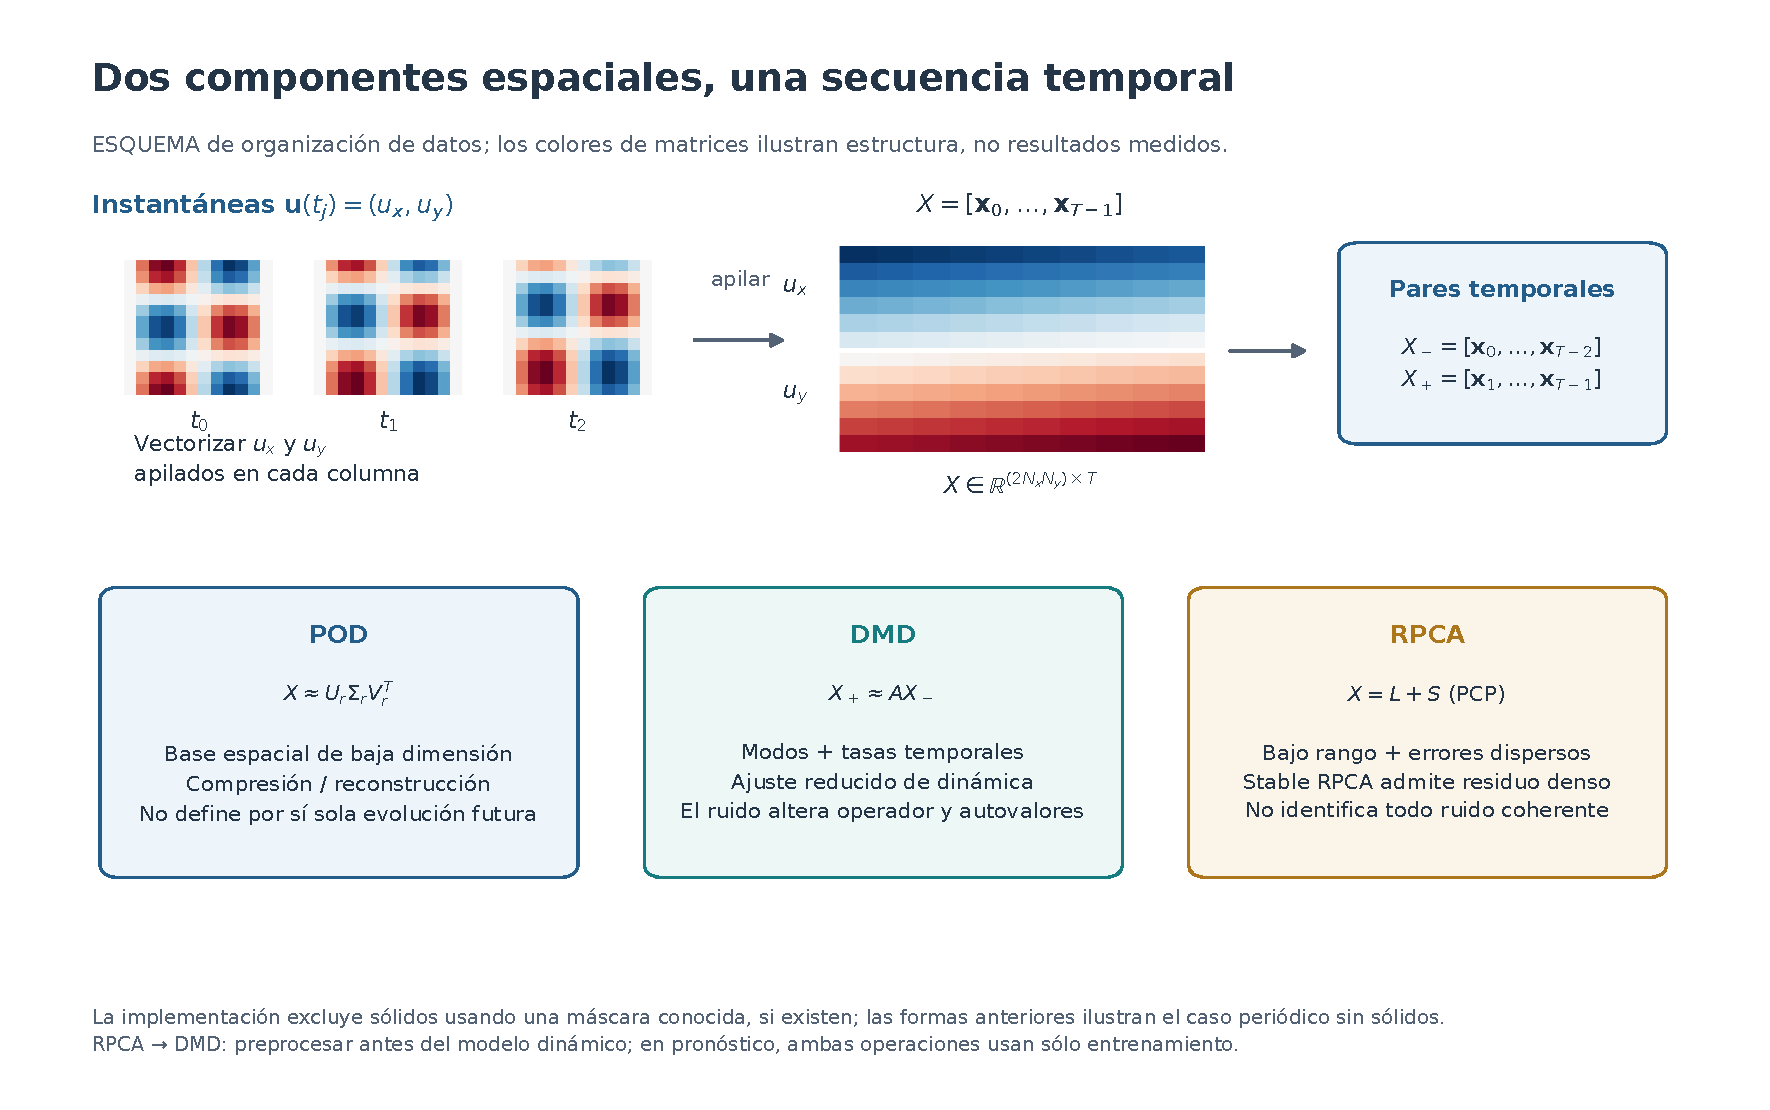
\includegraphics[width=\textwidth]{docs/research/figures/diagram_matrix_methods.pdf}
\caption{Representación esquemática de componentes y tiempos. POD, RPCA y DMD usan la misma organización de observaciones, pero imponen supuestos distintos. Los bloques coloreados son un esquema, no datos simulados.}
\label{fig:matrix-methods}\end{figure}

\section{PCP, RPCA estable y corrupción de columnas}
PCP modela una matriz de bajo rango más una componente dispersa:
\begin{equation}
 \min_{L,S}\norm{L}_*+\lambda\norm{S}_1
 \quad\text{sujeto a}\quad M=L+S.
 \label{eq:pcp}
\end{equation}
La norma nuclear suma valores singulares. Las condiciones de recuperación
de \citet{candes2011rpca} requieren identificabilidad, incluyendo restricciones
de estructura de bajo rango y soporte de corrupción. No expresan una
garantía universal para cualquier ruido. La implementación utiliza
umbralización singular y umbralización suave dentro de un esquema IALM,
registra su residuo y no equipara convergencia con error físico pequeño.

El SPCP estudiado por \citet{zhou2010stable} permite un residuo denso acotado:
\begin{equation}
 \min_{L,S}\norm{L}_*+\lambda\norm{S}_1,
 \qquad \norm{M-L-S}_F\leq\delta.
\end{equation}
El método local \code{stable_rpca} resuelve una formulación penalizada distinta:
\begin{equation}
 \min_{L,S}\frac12\norm{M-L-S}_F^2+
      \alpha\norm{L}_*+\beta\norm{S}_1.
 \label{eq:stable}
\end{equation}
Actualiza alternadamente $L$ por umbralización singular y $S$ por
umbralización entrada a entrada. El residuo denso no se fuerza a cero.
La formulación restringida y la penalizada están relacionadas por
regularización, pero no se traslada automáticamente la garantía de la
primera a cualquier elección de $\alpha$ y $\beta$ de la segunda.

Cuando se proporciona la intensidad relativa conocida $\epsilon$, el código
estima $\widehat\sigma=\epsilon\RMS(M)/\sqrt{1+\epsilon^2}$ y propone
$\alpha=\widehat\sigma(\sqrt m+\sqrt n)$ y
$\beta=\widehat\sigma\sqrt{2\log(mn)}$. Esta regla presupone una aproximación
de independencia para relacionar energía observada y señal; se informa como
heurística, especialmente fuera del ruido blanco.

Outlier Pursuit reemplaza la penalización de entradas por una penalización
de columnas \citep{xu2010outlier}:
\begin{equation}
 \min_{L,C}\norm{L}_*+\lambda\sum_{j=1}^n\norm{C_{:j}}_2,
 \qquad M=L+C.
\end{equation}
Una columna corresponde a un snapshot completo. Su objetivo de
recuperación es el subespacio y el soporte de columnas corruptas bajo sus
hipótesis; los valores limpios ocultos en una columna enteramente corrupta
no quedan identificados por esa observación. El piloto declara una cota
heurística $\gamma=0.1$ para la fracción de columnas y la regla
$\lambda=3/(7\sqrt{\gamma n})$; no verifica automáticamente todas las
condiciones del teorema de recuperación.

\section{DMD exacta y ajuste de amplitudes}
A partir de snapshots consecutivos se forman
\begin{equation}
 X=[m_0,\ldots,m_{n-2}],\qquad
 Y=[m_1,\ldots,m_{n-1}],\qquad Y\approx AX.
\end{equation}
Con $X=U_r\Sigma_rV_r^*$, la DMD reducida utiliza
\begin{equation}
 \widetilde A=U_r^*YV_r\Sigma_r^{-1},\quad
 \widetilde AW=W\Lambda,\quad
 \Phi=YV_r\Sigma_r^{-1}W.
\end{equation}
La evolución se representa mediante
$\widehat m_k=\Phi\diag(\lambda_1^k,\ldots,\lambda_r^k)b$.
Esta descripción conecta modos espaciales y tasas/frecuencias
\citep{schmid2010dmd}. En el piloto, las amplitudes se ajustan globalmente
en el intervalo observado. Que ese ajuste reduzca el residuo no prueba
capacidad predictiva en tiempos posteriores.

\section{TLS-DMD y forward--backward DMD}
El ruido de observación afecta tanto $X$ como $Y$; la regresión que sólo
considera errores en la segunda matriz puede inducir sesgo.
\citet{dawson2016noise} analizan este problema y proponen correcciones.

La variante TLS construye $Z=[X^T,Y^T]^T$, obtiene sus vectores singulares
derechos dominantes $V_{Z,r}$ y proyecta ambas matrices sobre el mismo
subespacio temporal:
\begin{equation}
 P=V_{Z,r}V_{Z,r}^*,\qquad X_c=XP,\qquad Y_c=YP.
\end{equation}
Después aplica DMD a $(X_c,Y_c)$. La selección de rango y el
condicionamiento continúan siendo relevantes.

La formulación forward--backward combina operadores en una base POD común.
Si $A_f$ aproxima $X\to Y$ y $A_b$ aproxima $Y\to X$, se considera
\begin{equation}
 A_{fb}^2=A_fA_b^{-1}.
\end{equation}
La raíz matricial no es única. La implementación elige en cada dirección
propia la rama más cercana a la dinámica directa, verifica el residuo de la
raíz y falla explícitamente cuando la inversión, la base propia o la
selección de rama son ambiguas o están mal condicionadas. No se ocultan
esos casos mediante reemplazo de valores no finitos.

\section{Optimized DMD y extensiones posteriores}
En coordenadas POD observadas, con $Q=(U_r^*M)^T$, se construye
$E(\omega)_{kj}=\exp(t_k\omega_j)$ y se resuelve
\begin{equation}
 \min_{\omega\in\C^r}\norm{Q-E(\omega)B(\omega)}_F^2,
 \qquad B(\omega)=E(\omega)^\dagger Q.
 \label{eq:optdmd}
\end{equation}
Es un ajuste exponencial con proyección variable
\citep{askham2018optimized}. La implementación usa mínimos cuadrados no
lineales con diferencias finitas, dos inicializaciones predeclaradas,
límites de tasas/frecuencias y presupuesto de evaluaciones. Reporta
convergencia y restricciones activas; no consulta el campo limpio para
escoger la inicialización.

La optimized DMD del piloto no es BOP-DMD. El bagging de
\citet{sashidhar2022bagging}, las pérdidas robustas dentro de DMD
\citep{askham2022robust}, las estructuras físicas de piDMD
\citep{baddoo2023physics}, los retardos de HODMD
\citep{leclainche2017hodmd}, Subspace DMD
\citep{takeishi2017subspace} y ResDMD
\citep{colbrook2023resdmd} constituyen extensiones diferenciadas.
Su inclusión posterior requiere identificar la formulación, verificarla y
contabilizar su costo. SPOD \citep{towne2018spod} aporta un análisis modal
dependiente de frecuencia para procesos estacionarios; no es por sí sola
un pronosticador de campos.

\section{Navier--Stokes y formulación vorticidad--función de corriente}
Para un fluido newtoniano incompresible de densidad constante,
\begin{equation}
 \nabla\cdot\boldsymbol u=0,\qquad
 \partial_t\boldsymbol u+\boldsymbol u\cdot\nabla\boldsymbol u
 =-\rho^{-1}\nabla p+\nu\Delta\boldsymbol u+\boldsymbol f.
\end{equation}
Los métodos de proyección separan el tratamiento de velocidad y presión
\citep{chorin1968ns}; los enfoques espectrales son antecedentes de DNS
\citep{orszag1972dns}. La implementación local se restringe al dominio
bidimensional periódico y a $\boldsymbol f=0$.

Se define $\omega=\partial_xv-\partial_yu$ y se usa
\begin{equation}
 u=\partial_y\psi,\quad v=-\partial_x\psi,\quad
 -\Delta\psi=\omega,\quad
 \partial_t\omega+u\partial_x\omega+v\partial_y\omega=\nu\Delta\omega.
\end{equation}
En Fourier, $\widehat\psi_{\boldsymbol k}
=\widehat\omega_{\boldsymbol k}/|\boldsymbol k|^2$ para
$\boldsymbol k\ne0$. La media de vorticidad se elimina para un campo
periódico compatible y la velocidad media se fija en cero. El término
no lineal utiliza dealiasing con corte estricto de dos tercios; la
integración es RK4, con paso limitado por CFL y difusión. Se registran
los subpasos efectivos.

En el toro cuadrado de lado $2\pi$, una referencia exacta es
\begin{align}
 u&=A\sin x\cos y\,e^{-2\nu t},\qquad
 v=-A\cos x\sin y\,e^{-2\nu t},\\
 p&=\frac{\rho A^2}{4}(\cos2x+\cos2y)e^{-4\nu t}.
\end{align}
La referencia Taylor--Green 2D verifica signos, derivación y difusión.
No equivale al desarrollo turbulento tridimensional del problema histórico
\citep{taylorgreen1937} ni prueba por sí sola la resolución del término
no lineal. Los vórtices interactuantes y la banda inicial de vorticidad se
integran numéricamente; deben acompañarse de refinamiento espacial y
temporal. La verificación con una solución exacta o manufacturada es un
ejercicio matemático distinto de validación física experimental
\citep{roache2002mms}.

\section{Canal Herschel--Bulkley y plug}
Se considera un canal $y\in[-H,H]$, no-slip en las paredes, gradiente de
presión $G=-\partial_xp$ y velocidad plenamente desarrollada $(u(y),0)$.
La constitutiva combina esfuerzo de cedencia $\tau_y$, consistencia $K$
e índice $n$ \citep{herschel1926bulkley}:
\begin{equation}
 \tau_{xy}=-Gy,\qquad
 \partial_yu=\operatorname{sgn}(\tau_{xy})
 \left(\frac{\max(|\tau_{xy}|-\tau_y,0)}{K}\right)^{1/n}.
\end{equation}
En el plug se cumple la desigualdad $|\tau_{xy}|\leq\tau_y$ y
$\partial_yu=0$; esto no implica esfuerzo nulo. Con $g=|G|$ y
$gH>\tau_y$, el perfil exacto es
\begin{equation}
 u(y)=\frac{\operatorname{sgn}(G)n}{(n+1)gK^{1/n}}
 \left[(gH-\tau_y)^{1+1/n}
 -\max(g|y|-\tau_y,0)^{1+1/n}\right].
\end{equation}
Si $gH\leq\tau_y$, el canal permanece sin flujo. El semiancho del
plug es $\min(H,\tau_y/g)$ para $g>0$. $K$ tiene unidades
Pa\,s$^n$, no siempre unidades de viscosidad newtoniana. El caso $n=1$
con $\tau_y>0$ representa Bingham; con $\tau_y=0$ recupera
Poiseuille newtoniano. El piloto usa $n=0.6,1,1.4$.

Estos campos se evalúan mediante la fórmula exacta. Son referencias
analíticas estacionarias, no DNS integradas en el tiempo ni ejemplos de
desprendimiento de vórtices. La regularización de
\citet{papanastasiou1987yield} es una alternativa para geometrías donde se
resuelven las ecuaciones numéricamente; no se necesita para evaluar este
perfil y no produce una superficie de cedencia exacta sin análisis de
su límite.

\section{Oldroyd-B: referencia de canal unidimensional}
La viscoelasticidad requiere memoria de esfuerzos y acoplamiento con el
momento; cambiar sólo la viscosidad no introduce esa física
\citep{oldroyd1950}. Para $\boldsymbol u=(u(y,t),0)$, esfuerzos inicialmente
nulos y $\tau_{yy}=0$, el módulo resuelve
\begin{align}
 \rho\partial_tu&=\eta_s\partial_{yy}u+
                     \partial_y\tau_{xy}+G(t),\\
 \lambda\partial_t\tau_{xy}+\tau_{xy}&=\eta_p\partial_yu,\\
 \lambda\partial_t\tau_{xx}+\tau_{xx}&=
                  2\lambda(\partial_yu)\tau_{xy}.
 \label{eq:oldroyd1d}
\end{align}
La velocidad se discretiza en nodos y los esfuerzos en caras; se aplica
Euler implícito acoplado, de primer orden temporal y segundo espacial.
La ecuación de esfuerzo cortante se elimina antes de resolver el sistema
tridiagonal de velocidad. Los residuos del acoplamiento se miden en los
pasos internos, no sólo diferenciando snapshots espaciados. Con
$\lambda=0$ se recupera viscosidad newtoniana $\eta_s+\eta_p$.

Para $G$ constante, el estado estacionario verifica
$u=G(H^2-y^2)/(2(\eta_s+\eta_p))$,
$\tau_{xy}=\eta_p\partial_yu$ y
$\tau_{xx}=2\lambda\eta_p(\partial_yu)^2$.
La solución de arranque, el límite newtoniano y el refinamiento aportan
pruebas de esta reducción. No hay advección de esfuerzos alrededor de un
obstáculo ni interacción con una estela 2D.

La ampliación actual incorpora FENE-P y extensibilidad finita en un dominio
periódico bidimensional \citep{bird1980fenep}. Las constitutivas EVP de
\citet{saramito2007evp,saramito2009hb} siguen pendientes. Para wakes viscoelásticos se
considera log-conformation \citep{fattal2004log,fattal2005time}, con
positividad y resolución del tensor. La existencia de solvers como
RheoTool \citep{pimenta2017rheotool,rheotoolCode} o Basilisk
\citep{basiliskLogConformation} no implica que ya estén integrados o
ejecutados en esta campaña.

\section{Memoria viscoelástica bidimensional acoplada}
La nueva implementación resuelve velocidad y conformación polimérica en el
toro periódico, con densidad adimensional uno. La velocidad es planar y el
tensor constitutivo es por defecto $C\in\R^{3\times3}$, incluyendo $C_{zz}$:
\begin{align}
 \partial_t\boldsymbol u+\boldsymbol u\cdot\nabla\boldsymbol u
  &=-\nabla p+\nu_s\Delta\boldsymbol u+\nabla\cdot\tau_p,
  &\nabla\cdot\boldsymbol u&=0,\\
 \partial_tC+\boldsymbol u\cdot\nabla C
  &=GC+CG^T-\frac{f(C)C-I}{\lambda}+\kappa\Delta C,
  &G_{ij}&=\partial_j u_i,\\
 \tau_p&=\frac{\nu_p}{\lambda}(f(C)C-I).
\end{align}
Oldroyd-B utiliza $f=1$; FENE-P utiliza
$f=(L^2-3)/(L^2-\tr C)$, con $C\succ0$ y $\tr C<L^2$.
Esta normalización hace que $C=I$ tenga esfuerzo cero. La extensión finita
modifica también $C_{zz}$ aunque la velocidad sólo tenga dos componentes.

Se integra con RK4, colocación de Fourier y proyección solenoidal. El paso
interno está limitado por advección, difusión, relajación, estiramiento y una
escala elástica. Cada etapa exige conformación finita, simétrica, positiva y
traza admisible. Una violación rechaza el paso y reduce su tamaño; nunca se
reparan silenciosamente autovalores o traza. La difusión de conformación
$\kappa$ es una modificación explícita del modelo; vale cero en las campañas.
El factor racional de FENE-P no queda exactamente desaliasado mediante corte
2/3: se conserva su defecto de cuadratura/proyección en los diagnósticos.

La energía polimérica de Oldroyd-B es
\begin{equation}
 E_p=\frac{\nu_p}{2\lambda}\langle\tr C-\log\det C-3\rangle.
\end{equation}
Se verifica el intercambio entre energía cinética y polimérica, relajación
disipativa, cizalla homogénea analítica, límite newtoniano y refinamientos
espaciales/temporales. Los residuos constitutivos derivados de instantáneas
se distinguen de los residuos del integrador. Los detalles y datos están en
\path{docs/research/VISCOELASTIC_2D.md} y
\path{results/research/solver_validation_2d/viscoelastic.json}.

\section{Momentum viscoplástico bidimensional regularizado}
El segundo solver integra una constitutiva inelástica con esfuerzo completo
variable; no reescala una trayectoria newtoniana. Para
$D=(\nabla\boldsymbol u+\nabla\boldsymbol u^T)/2$ y
$\dot\gamma=\sqrt{2D:D}$, resuelve
\begin{align}
 \partial_t\boldsymbol u+\boldsymbol u\cdot\nabla\boldsymbol u
  &=-\rho^{-1}\nabla p+\rho^{-1}\nabla\cdot(2\eta_{app}D),\\
 \eta_{app}&=\eta_s+K(\dot\gamma^2+\epsilon^2)^{(n-1)/2}
  +\tau_y\frac{1-e^{-m\dot\gamma}}{\dot\gamma}.
\end{align}
El término de cedencia se evalúa por su límite $\tau_y m$ en corte cero,
sin cap de viscosidad. $n=1$ representa Bingham regularizado; $n<1$ y $n>1$
permiten adelgazamiento y espesamiento. $m$ y $\epsilon$ modifican la
regularización y requieren estudios distintos del refinamiento de malla.

El esquema usa RK4 adaptativo por estabilidad, esfuerzo en cuadratura
ampliada y proyección de presión. La cuadratura elimina productos
cuadráticos retenidos, pero no todos los armónicos de la ley no polinómica.
Se informa su sensibilidad por separado. El balance periódico sin forzado es
\begin{equation}
 \frac{d}{dt}\frac{\rho}{2}\langle|\boldsymbol u|^2\rangle
  =-\langle\eta_{app}\dot\gamma^2\rangle\le0.
\end{equation}
La superficie de cedencia sólo se estima con umbrales declarados: una ley
regularizada no produce regiones rígidas exactamente no cedidas. La
convergencia espacial observada es modesta y no acredita una DNS resuelta.
La implementación y sus controles están en
\path{docs/research/VISCOPLASTIC_2D.md} y
\path{results/research/solver_validation_2d/viscoplastic.json}.

\begin{figure}[htbp]\centering
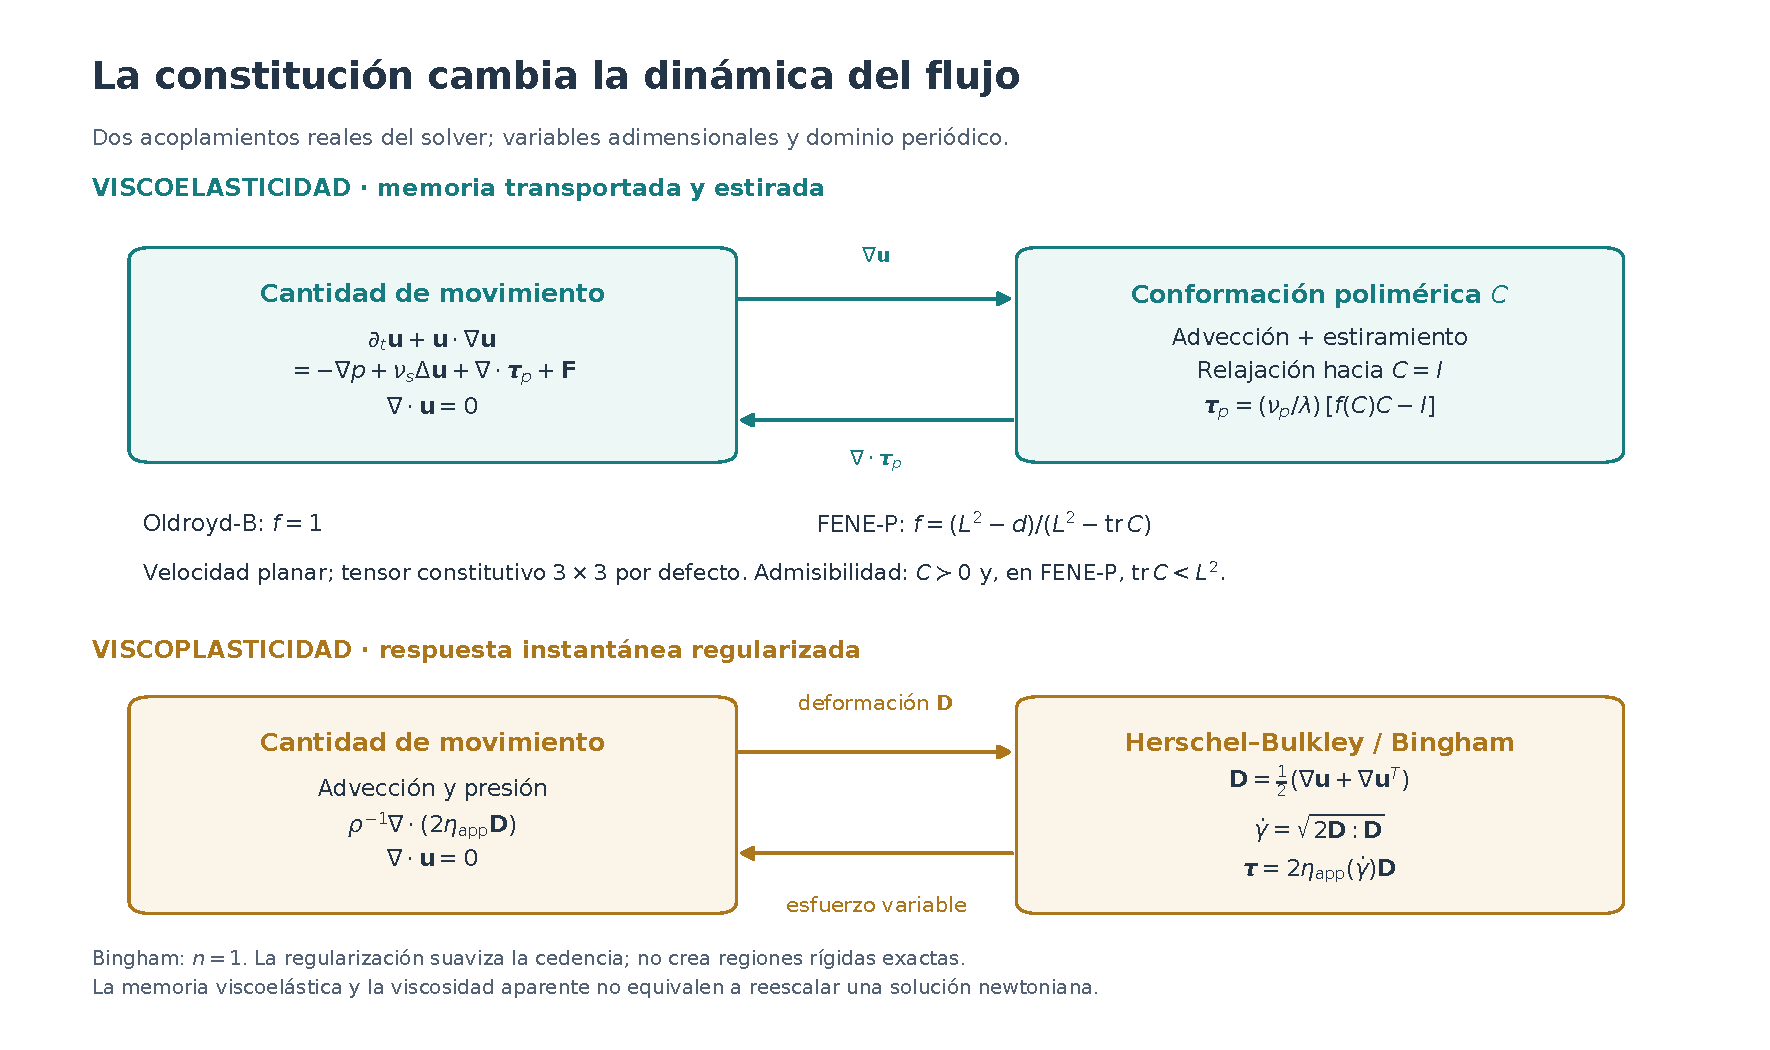
\includegraphics[width=\textwidth]{docs/research/figures/diagram_constitutive_loop.pdf}
\caption{La memoria polimérica realimenta el momento; la viscoplasticidad integra un esfuerzo variable instantáneo. Ambos acoplamientos modifican la evolución espacial, y no equivalen a reescalar una trayectoria newtoniana.}
\label{fig:constitutive-loop}\end{figure}

\section{Proyección física y residuo de movimiento}
Para dominios periódicos sin sólidos, la proyección de Helmholtz usa sólo la
geometría y elimina la componente longitudinal:
\begin{equation}
 \widehat{P\boldsymbol u}_{\boldsymbol k}
  =\widehat{\boldsymbol u}_{\boldsymbol k}
   -\boldsymbol k\frac{\boldsymbol k\cdot
    \widehat{\boldsymbol u}_{\boldsymbol k}}{|\boldsymbol k|^2}.
\end{equation}
La media se conserva; un corte 2/3 adicional es un prior de banda física
declarado antes de observar el test. No utiliza velocidad limpia ni se aplica
a canales o máscaras con obstáculos. En mallas pares, las primeras derivadas
usan el operador real compatible, con Nyquist nulo; el Laplaciano difusivo
conserva los números de onda completos. Confundir ambos operadores
subestimaría la difusión de modos Nyquist.

Para Newtoniano se calcula un residuo de vorticidad sin presión, mediante
derivación temporal de las instantáneas y operadores espaciales. Se informa
también el residuo adicional respecto al limpio, heredando su error de
discretización. Una reconstrucción sólo de velocidad no permite certificar
la PDE no newtoniana omitiendo el esfuerzo desconocido; esos residuos se
marcan como no disponibles en vez de aplicar una ecuación newtoniana falsa.

\section{Observables físicos y densidad}
Para reconstrucción $\widehat{\boldsymbol u}$ y referencia
$\boldsymbol u_{\mathrm{ref}}$, se mide
\begin{equation}
 e_u=\frac{\norm{\widehat{\boldsymbol u}-\boldsymbol u_{\mathrm{ref}}}_2}
                  {\norm{\boldsymbol u_{\mathrm{ref}}}_2},\qquad
 e_\omega=\frac{\norm{\widehat\omega-\omega_{\mathrm{ref}}}_2}
                      {\norm{\omega_{\mathrm{ref}}}_2}.
\end{equation}
Estas normas se calculan sobre nodos de fluido y, para vorticidad,
nodos válidos de derivación. El código usa derivadas espectrales en ejes
periódicos y diferencias de segundo orden en ejes no periódicos. Cuando
hay obstáculo, excluye un halo de una celda y usa diferencias locales.
El mismo operador se aplica a referencia y reconstrucción. Si un
denominador es cero con error no nulo, se informa métrica indefinida,
sin introducir un pequeño número que oculte esa situación.

La medida normalizada de divergencia adicional del piloto es
\begin{equation}
 d_{\mathrm{extra}}=
 \frac{\RMS(\nabla\cdot\widehat{\boldsymbol u}
              -\nabla\cdot\boldsymbol u_{\mathrm{ref}})}
      {\RMS(\omega_{\mathrm{ref}})}.
\end{equation}
Se informa también divergencia absoluta. Restar el residuo de referencia
ayuda a distinguir alteraciones de reconstrucción del residuo de datos
limpios, pero no certifica el solver.

Con pesos de integración $w_i$, por unidad de profundidad,
\begin{equation}
 M_\Omega=\sum_i\rho_iw_i,\qquad
 E=\frac12\sum_i\rho_i|\boldsymbol u_i|^2w_i,\qquad
 Z=\frac12\sum_{i\,\text{válido}}\omega_i^2w_i.
\end{equation}
Se utilizan rectángulos periódicos y trapecios sobre ejes nodales no
periódicos. El balance global de materia es
\begin{equation}
 B_M=\frac{dM_\Omega}{dt}+
        \int_{\partial\Omega}\rho\boldsymbol u\cdot\boldsymbol n\,ds.
\end{equation}
Las caras periódicas se emparejan. El flujo se normaliza con
$\overline\rho\,U_{\mathrm{ref,RMS}}\sqrt{|\Omega_{\mathrm{fluido}}|}$.
La reconstrucción del piloto sólo modifica velocidad; si copia densidad
de referencia, la fidelidad de masa es condicional a esa suposición.
Con densidad constante, $M_\Omega=\rho|\Omega|$ es trivial y no prueba
conservación de la velocidad reconstruida.

El flujo neto puede cancelar entradas y salidas no físicas por paredes.
En canales se evalúan por separado velocidad de pared y penetración
normal, normalizadas por la velocidad RMS del volumen. En el LBM legacy
se asume flujo nulo sobre el sólido y el área se aproxima mediante su
máscara; no se pretende una integración exacta del esfuerzo o la fuerza
sobre el cilindro. Calcular residuo de momento, lift o drag exige presión,
esfuerzos y condiciones de contorno compatibles; no se deducen
automáticamente de estos diagnósticos de velocidad.

\chapter{Desarrollo experimental}
\section{Piloto preservado y procedencia física}
Esta sección describe el baseline anterior, conservado con su procedencia en
\path{results/research/baseline_2026-10-14/}; sus cifras no se atribuyen a una
nueva ejecución de reissued. La tabla~\ref{tab:cases} resume sus ocho casos. Una malla se
expresa como $N_x\times N_y$. El dominio periódico NS tiene lado $2\pi$;
los canales reológicos tienen $H=1$, longitud $2$, $\rho=1$, $G=1$ y,
para HB, $K=1$ y $\tau_y=0.2$ en unidades consistentes.

\begin{table}[htbp]
\centering\small
\caption{Banco piloto: configuraciones, no certificaciones automáticas de DNS.}
\label{tab:cases}
\begin{tabular}{@{}p{3.8cm}p{1.7cm}p{7.8cm}@{}}
\toprule
Caso & Malla & Referencia y parámetros\\
\midrule
Taylor--Green NS & $24\times24$ & Integración NS; $\nu=0.05$, $\Delta t=0.01$,
  150 pasos, muestra cada 5; comparación analítica.\\
Vórtices interactuantes & $48\times48$ & Integración NS de cuatro núcleos
  periodizados; $\nu=0.02$, mismo tiempo/muestreo.\\
Banda de vorticidad en decaimiento & $64\times64$ & Integración NS,
  semilla física 19, $\nu=0.02$; el nombre del caso no acredita turbulencia resuelta.\\
Arranque Oldroyd-B & $8\times33$ & Reducción 1D; $\eta_s=\eta_p=0.5$,
  $\lambda=0.5$, $\Delta t=0.01$, 300 pasos, muestra cada 10.\\
HB shear-thinning & $8\times33$ & Perfil exacto estacionario,
  $n=0.6$; snapshots repetidos cada $0.05$ hasta $1.5$.\\
Bingham & $8\times33$ & Perfil exacto estacionario, $n=1$;
  mismo muestreo nominal.\\
HB shear-thickening & $8\times33$ & Perfil exacto estacionario,
  $n=1.4$; mismo muestreo nominal.\\
Cilindro LBM legacy & $80\times40$ & D2Q9--BGK conservado,
  $Re=80$, $u_{\mathrm{in}}=0.06$, 1100 pasos,
  warmup 500, muestra cada 20.\\
\bottomrule
\end{tabular}
\end{table}

Los siete primeros casos producen 31 snapshots según la configuración.
El LBM legacy conserva sus fronteras: streaming transversal periódico,
entrada de equilibrio y salida por copia. Su metadata lo identifica como
referencia no validada. No se sustituye esa geometría por el benchmark
Schäfer--Turek \citep{schaefer1996cylinder} ni se comparan sus coeficientes
con valores de un cilindro con otras fronteras.

\section{Contaminación con presupuesto de energía comparable}
El piloto preservado genera seis modelos de ruido de observación, todos con intensidad
$\epsilon=0.2$. Después de generar su estructura, se normaliza la RMS
realizada sobre componentes y nodos de fluido:
\begin{equation}
 M_{\mathrm{obs}}=M_{\mathrm{clean}}+N,\qquad
 \frac{\RMS(N)}{\RMS(M_{\mathrm{clean}})}=0.2.
\end{equation}
Esta convención equivale a aproximadamente $13.98$ dB de SNR basado en
energía. Igualar RMS no hace equivalentes las distribuciones o las
correlaciones; permite separar presupuesto energético y estructura.

\begin{enumerate}
\item Gaussiano denso, generado inicialmente con entradas independientes y
      luego renormalizado a la energía declarada.
\item Impulsivo disperso, con selección Bernoulli de probabilidad $0.05$.
\item Mixto, con fracciones de energía esperada $0.5$ gaussiana y $0.5$
      impulsiva antes de la normalización final.
\item Correlacionado espacialmente, mediante filtro gaussiano de escala
      $1.5$ celdas y extensión periódica del ruido generado.
\item Correlacionado temporalmente, mediante AR(1):
      $N_k=0.8N_{k-1}+\sqrt{1-0.8^2}\,\xi_k$, con inicio estacionario.
\item Outliers por columna, seleccionando snapshots completos;
      se contamina $\max(1,\lceil0.05n\rceil)$ de ellos.
\end{enumerate}
La fracción realizada de columnas se registra: en una serie corta no
necesariamente coincide exactamente con $5\%$. La correlación espacial
periódica es una decisión del experimento de observación, no una afirmación
sobre las fronteras físicas de un sensor real.

Este ruido se añade a un campo ya calculado. Una perturbación del forzado,
la condición inicial o la constitutiva es un experimento físico diferente
y requiere integrar de nuevo el sistema. Las semillas de contaminación
son 7, 23 y 61; no se confunden con la semilla 19 de la condición inicial
del caso en decaimiento.

\section{Estimadores y presupuesto}
\begin{table}[htbp]
\centering\small
\caption{Once métodos o cadenas del piloto preservado.}
\begin{tabular}{@{}p{3.9cm}p{9.3cm}@{}}
\toprule Método & Función\\\midrule
\code{identity} & Observación sin limpiar: baseline de daño.\\
\code{pod} & Aproximación SVD de rango solicitado.\\
\code{rpca} & PCP restringido a $M=L+S$ mediante IALM.\\
\code{stable_rpca} & Modelo penalizado bajo rango + disperso + residuo denso.\\
\code{outlier_pursuit} & Corrupción de columnas, penalización $\ell_{2,1}$.\\
\code{dmd} & DMD exacta con amplitudes globales.\\
\code{tls_dmd} & Proyección TLS de $X$ e $Y$, seguida de DMD.\\
\code{fb_dmd} & Operador forward--backward en base común; raíz verificada.\\
\code{optimized_dmd} & Ajuste exponencial por proyección variable.\\
\code{rpca_dmd} & PCP seguido de DMD.\\
\code{stable_rpca_dmd} & RPCA estable penalizada seguida de DMD.\\
\bottomrule
\end{tabular}
\end{table}

En el piloto preservado el rango solicitado es cuatro para métodos que lo usan. Para los convexos
se registra el rango efectivo seleccionado por regularización. Se fija
tolerancia $10^{-5}$ y hasta 600 iteraciones; optimized DMD tiene dos
inicios y presupuesto de 100 evaluaciones por inicio, con diagnósticos de
su optimizador. Cada réplica tiene un límite de ajuste de 90 segundos.
Esos límites forman parte del ensayo y un método que los excede permanece
identificado como fracaso o ausencia de convergencia.

El diseño nominal es $8\times6\times3\times11=1584$ condiciones, cada una
con tres repeticiones de recursos: hasta 4752 ajustes. Estos conteos
describen la configuración; el capítulo de resultados informa cuántos
se ejecutaron efectivamente y cuántos convergieron. No se reemplazan
resultados fallidos por el mejor ensayo ni se confunden tres réplicas de
una misma entrada con nuevas realizaciones de ruido.

\section{Ampliación ejecutada: flujos 2D y nuevas contaminaciones}
La configuración de reconstrucción actual mantiene los tres casos
newtonianos del piloto y sustituye las referencias de canal/legacy por cinco
flujos periódicos realmente integrados. Oldroyd-B y FENE-P utilizan malla
$32^2$, $\nu_s=.02$, $\nu_p=.04$, $\lambda=.5$, amplitud RMS inicial $.6$,
$\Delta t=.005$ y duración $.6$; FENE-P usa $L^2=12$. Los tres flujos
viscoplásticos utilizan $32^2$, $K=.02$, $\tau_y=.02$, $m=10$,
$\epsilon=.001$, índices $.6,1,1.4$, paso nominal $.005$ y duración $2$.
Los tiempos de muestreo y parámetros completos están en la configuración.

A las seis contaminaciones del piloto se agregan Student-$t$ con tres
grados de libertad, ruido heteroscedástico y deriva de sensor coherente.
Todas tienen presupuesto RMS realizado del 20\% para reconstrucción.
Colas pesadas, dependencia y sesgo cambian las hipótesis de identificación:
una deriva coherente puede ser de bajo rango y no distinguirse de la señal
mediante ese supuesto solamente. Las semillas siguen siendo 7, 23 y 61.

Se predeclaran 13 opciones: identity, POD, PCP, RPCA estable, DMD exacta,
TLS-DMD, optimized DMD, un dispatcher fbDMD con alternativa TLS explícita,
identity/POD/TLS/RPCA estable con Helmholtz y TLS con Helmholtz más corte 2/3.
El dispatcher conserva el fallo primario y suma el trabajo de ambos métodos;
no registra esa recuperación como éxito puro de fbDMD. Outlier Pursuit y las
cadenas RPCA--DMD permanecen implementadas y evaluadas en el piloto, aunque
no integran las 13 opciones de esta campaña. Los convexos tienen hasta
1200 iteraciones y optimized DMD dos inicios de hasta 200 evaluaciones;
la tolerancia permanece $10^{-5}$ y el rango solicitado cuatro.

El diseño ejecutado es $8\times9\times3\times13=2808$ condiciones,
con tres repeticiones de recursos: 8424 ajustes. El costo medido incluye
reconstrucción, retorno a campos vectoriales y posprocesamiento físico.
Evaluación contra referencia y escritura de artefactos se contabilizan
fuera del ajuste. No se intercambian las cifras de esta campaña con las
1584 condiciones del piloto preservado.

\section{Pronóstico sin acceso al futuro y control reológico común}
La campaña de pronóstico separa cronológicamente 60\% de entrenamiento,
20\% de validación y el resto de prueba. Evalúa cinco flujos (vórtices
newtonianos, Taylor--Green Oldroyd-B/FENE-P y vórtices Oldroyd-B/FENE-P),
cuatro ruidos y tres semillas: 60 escenarios. Las 29 opciones predeclaradas
incluyen persistencia, POD autorregresivo ridge, DMD exacta/TLS/optimizada,
preprocesamiento RPCA sólo en entrenamiento y variantes físicas. Los rangos
son dos, cuatro y ocho. Los ajustes compartidos entre variantes físicas no
se cuentan como entrenamientos independientes.

La escala de contaminación se calibra sólo con la RMS de entrenamiento;
el proceso temporal es causal y el soporte de outliers no depende de valores
futuros. La selección minimiza error sobre validación ruidosa, sin usar
referencia limpia ni observaciones de prueba y sin reajuste posterior.
La interpretación de ese criterio como riesgo limpio requiere ruido de
validación independiente y de media cero; no se presume para ruido AR(1).
La persistencia filtrada controla cuánto beneficio procede del prior
espacial. El costo de pronóstico mide la evaluación completa de candidatos
en un proceso aislado, con una réplica por escenario, y no tiempos aislados
de cada estimador.

Una campaña adicional compara seis constitutivas con la misma velocidad
inicial, densidad, dominio, malla $32^2$ y 31 tiempos hasta $1.2$.
Newtoniano, Oldroyd-B y FENE-P comparten viscosidad nominal $.06$;
las consistencias HB se ajustan para igualar esa viscosidad aparente en una
tasa de corte declarada. Esto no iguala toda su respuesta constitutiva.
Los cambios respecto al Newtoniano son diferencias físicas simuladas, no
errores de reconstrucción. La animación y las tablas se conservan en
\path{results/research/rheology_matched_2026-10-14/}.

\begin{figure}[htbp]\centering
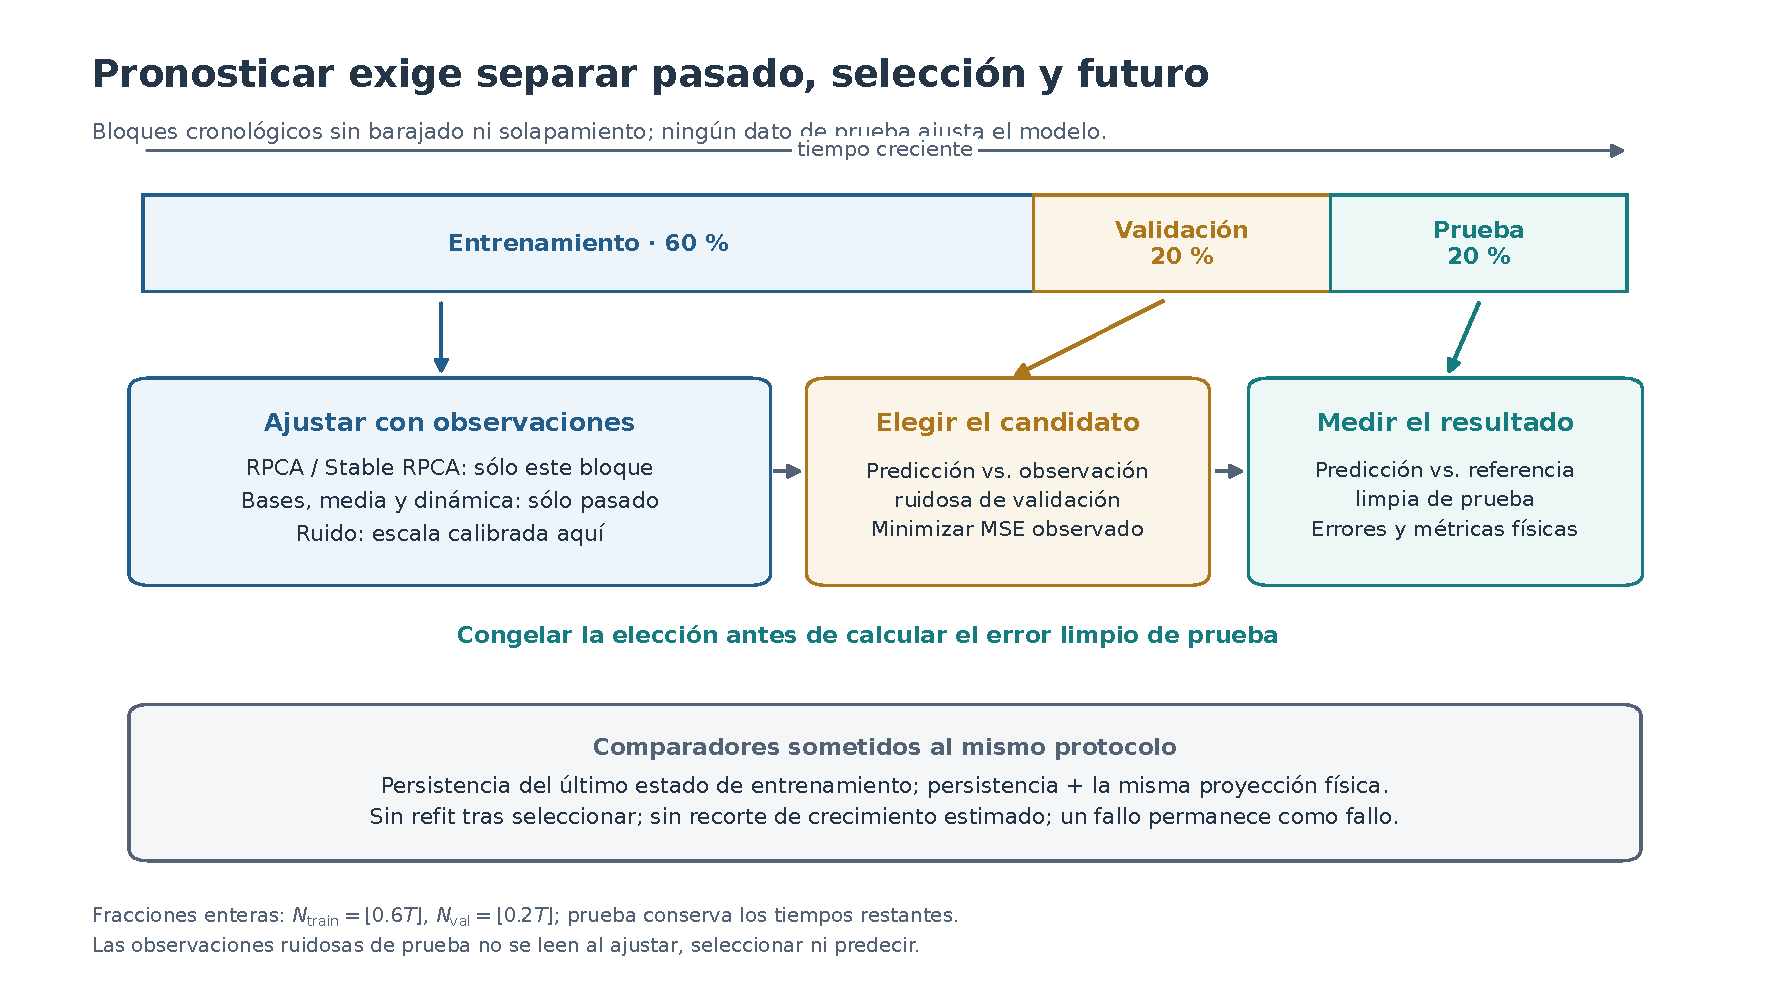
\includegraphics[width=\textwidth]{docs/research/figures/diagram_chronological_protocol.pdf}
\caption{Separación cronológica: la limpieza y el ajuste ven sólo entrenamiento; la elección utiliza validación ruidosa; la referencia limpia futura evalúa después de seleccionar. La observación de prueba no se utiliza para reajustar.}
\label{fig:chronological-protocol}\end{figure}

\section{Campañas de mayor resolución y evolución espacial}
La ampliación visual ejecuta cada malla mediante una nueva integración del
sistema. Comparar imágenes interpoladas de un único campo no equivale a
resolver el flujo de nuevo. Se mantienen dentro de cada estudio dominio,
condición inicial física, constitutiva y tiempos de salida; se modifica la
malla, con los subpasos internos limitados por estabilidad.

El banco newtoniano compara $64^2,128^2,256^2,512^2$ en dos condiciones
no lineales, con velocidad RMS inicial $.8$, viscosidad $.01$, lado $2\pi$
y duración $4$. Conserva 41 instantáneas. Las referencias Oldroyd-B/FENE-P
comparan $64^2,128^2,256^2$ hasta $2.4$, con 25 instantáneas, RMS inicial
$.8$, $\nu_s=.02$, $\nu_p=.04$, $\lambda=.5$, $L^2=12$ y $\kappa=0$.
No se confunden estas condiciones con los parámetros de los bancos anteriores.

Los flujos HB/Bingham tienen trayectorias $64^2$ y $128^2$ hasta $2$, con
21 instantáneas. La referencia adicional $256^2$ sólo alcanza $.1$ por el
costo del esquema explícito con viscosidad aparente variable. Verifica un
intervalo corto y no certifica automáticamente la evolución larga de $128^2$.
La viscosidad nominal aparente se iguala en la tasa de corte declarada a
$.04$, con $\tau_y=.01$, $m=10$, $\epsilon=.001$ y RMS inicial $.8$.
Estos parámetros difieren del banco viscoelástico; los contrastes entre
familias no se presentan como una comparación reológica controlada única.

\begin{figure}[htbp]\centering
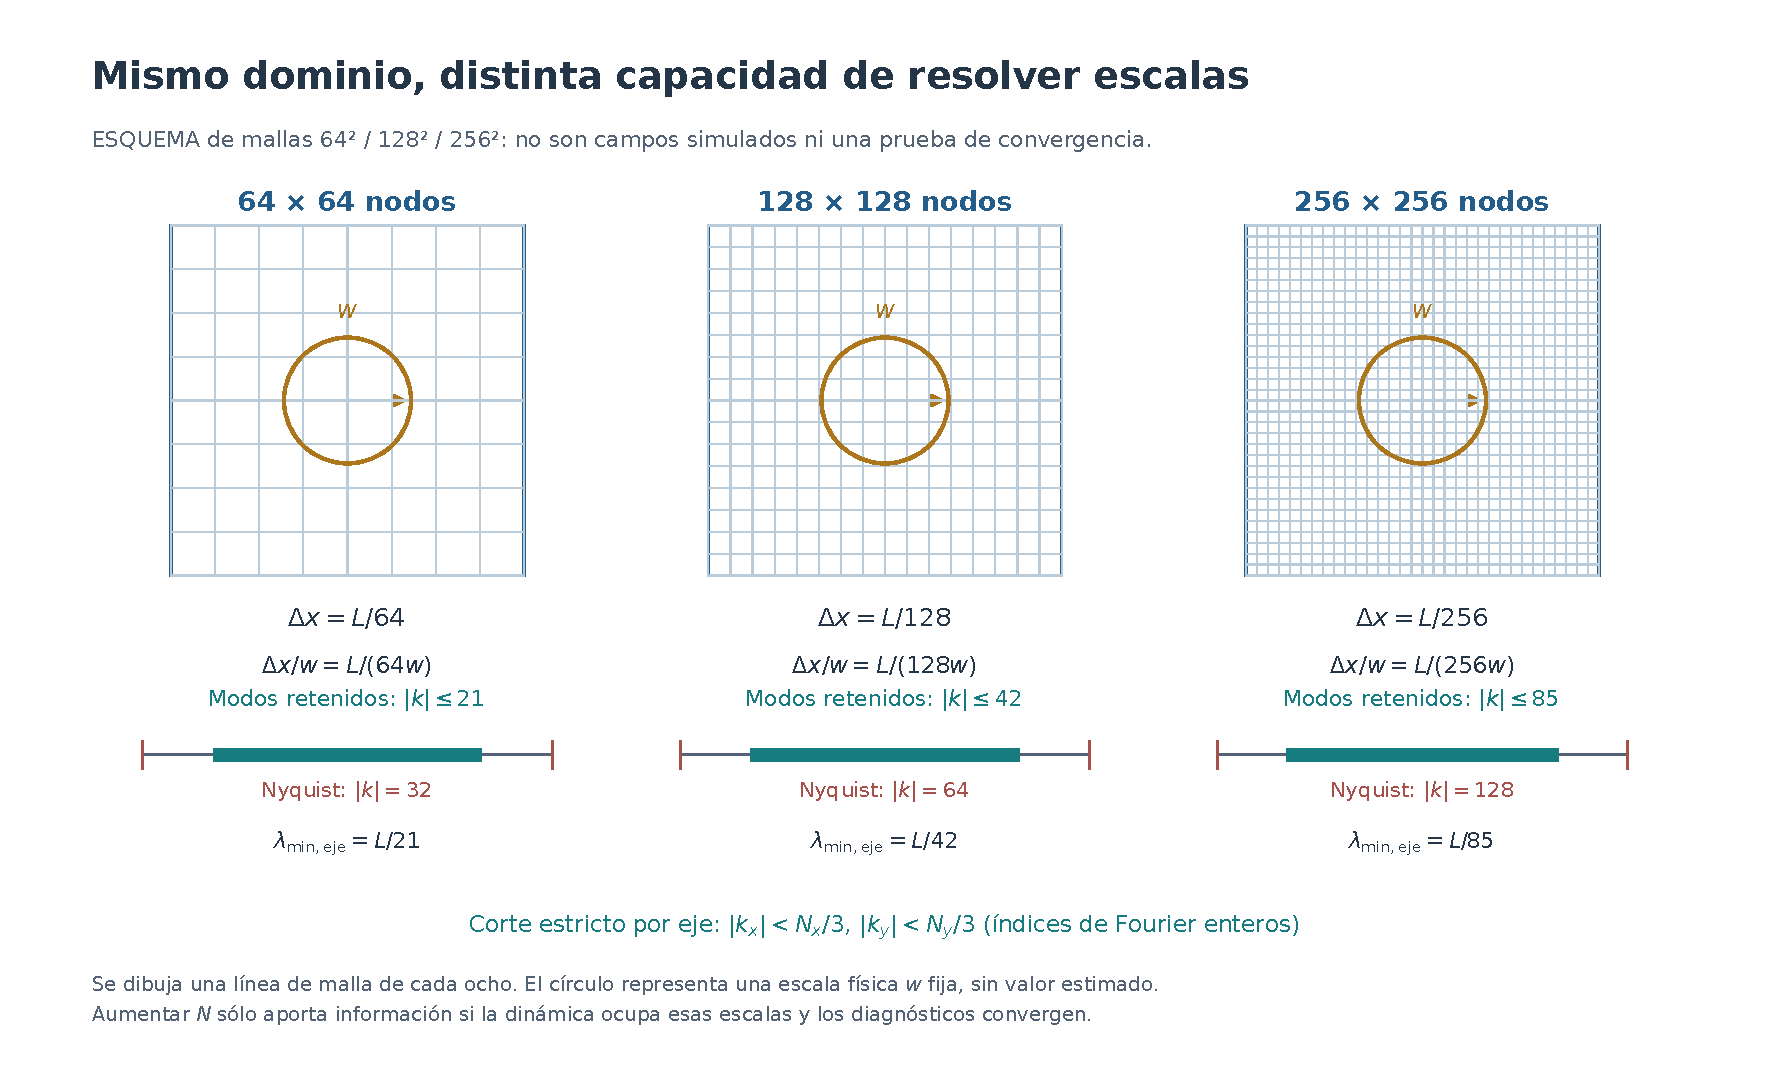
\includegraphics[width=\textwidth]{docs/research/figures/diagram_spectral_resolution.pdf}
\caption{Relación entre dominio, escala física y resolución. Las mallas dibujadas son esquemas. El número de nodos y el corte 2/3 por eje describen la capacidad de representación; la convergencia exige además comparar campos y observables.}
\label{fig:spectral-resolution}\end{figure}

Se muestran dos errores espaciales: los modos que ambas mallas pueden
representar, y el campo completo de la referencia fina frente al grueso
prolongado por Fourier. El segundo incluye las estructuras que el grueso no
resuelve. La interpolación se emplea para comparar soluciones independientes,
no para generar nuevos datos. Se conservan curvas y máximos sobre todos los
tiempos muestreados: el estado final por sí solo puede ocultar picos intermedios.

La velocidad se acompaña de vorticidad, energía, enstrofía y espectros; en
viscoelasticidad también de $C-I$, esfuerzos, autovalor mínimo, traza y defectos
constitutivos. Comparar sólo $C$ puede ocultar deformación pequeña detrás de
la identidad. En HB/Bingham se examinan viscosidad aparente, tasa de corte,
esfuerzo y disipación. Una medida relativa con referencia nula se registra
como indefinida y se acompaña de error absoluto.

El ancho inicial $\sigma=.065L$ de los núcleos tiene 2.08 celdas en la
malla anterior de $32^2$, frente a 4.16, 8.32, 16.64 y 33.28 en las nuevas
$64^2,128^2,256^2,512^2$. Esa relación hace concreto el refinamiento,
pero los filamentos y esfuerzos pueden generar escalas menores durante el flujo.

La lectura exploratoria utiliza 1\% como tolerancia de velocidad/vorticidad
frente a la referencia numérica, y examina separadamente colas espectrales y
errores temporales. Son decisiones operativas de estos casos, no una
certificación DNS, una preregistración ciega o una regla universal de
representatividad. La duración, geometría, esfuerzo y régimen deben formar
parte de cualquier afirmación de suficiencia.

\begin{figure}[htbp]\centering
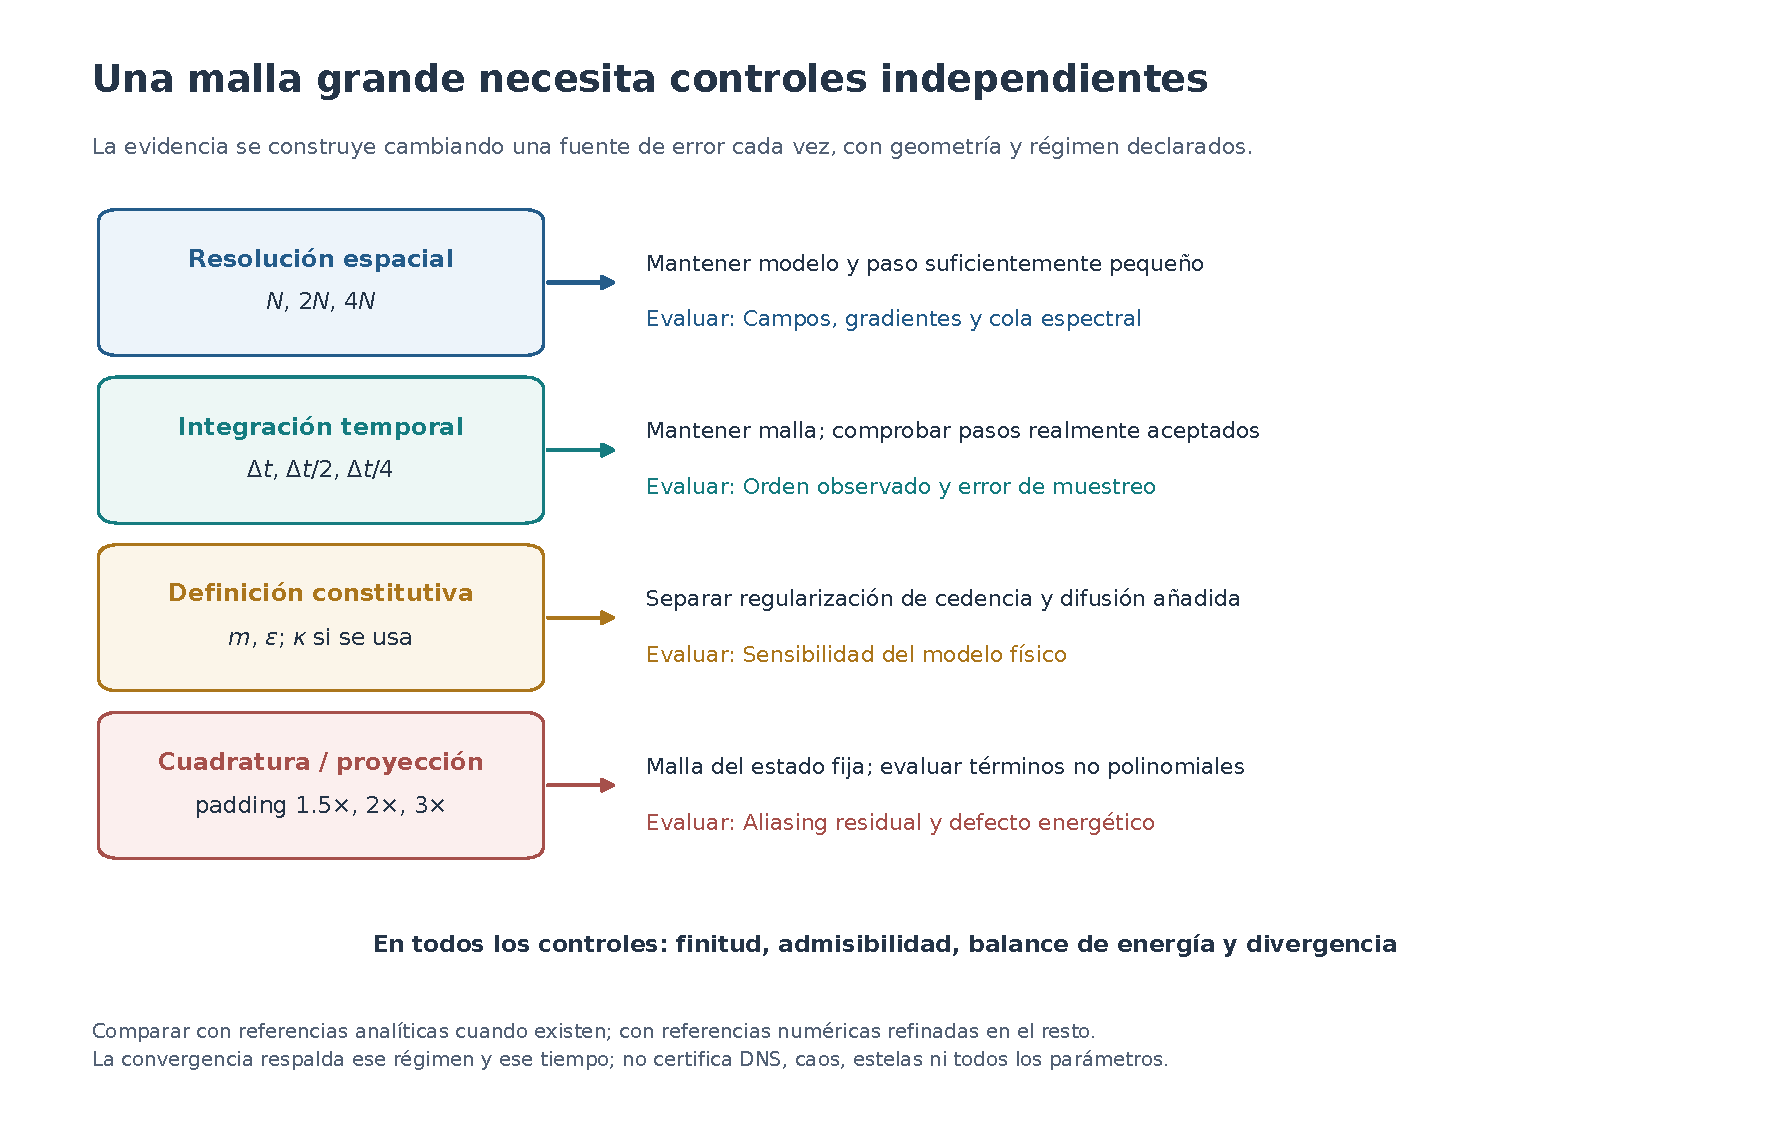
\includegraphics[width=\textwidth]{docs/research/figures/diagram_independent_checks.pdf}
\caption{Controles distintos para causas distintas de error. Malla, paso efectivo, cuadratura y regularización no se sustituyen entre sí. Una simulación finita o con balance discreto pequeño todavía puede estar espacialmente subresuelta.}
\label{fig:independent-checks}\end{figure}

La demostración de reconstrucción añade 60 condiciones sobre campos
$128^2$ y $256^2$, cinco estimadores o variantes y tres semillas. Contrasta
ruido gaussiano independiente por celda con ruido espacial generado por un
filtro gaussiano de ancho físico $\sigma_f=.10$. El ancho del filtro no es
el de la autocorrelación: en el límite continuo gaussiano, la desviación
estándar de ésta es $\sqrt2\sigma_f$. En el segundo, una misma realización sobre $256^2$ se
transfiere a $128^2$, sin renormalizar cada malla. Para el primero, refinar
la observación cambia su contenido de altas frecuencias: RMS igual no hace
equivalentes sus errores de derivadas. Los rangos ocho y dieciséis se fijan
antes de evaluar; esta limpieza utiliza el intervalo observado y no es una
campaña de pronóstico. El costo tiene una sola réplica sobre un host ocupado
por las simulaciones: no se presenta como una clasificación precisa de tiempos.

\section{Costo computacional y Pareto}
El vector de costo registra tiempo wall, CPU, RSS pico absoluta del
proceso, memoria visible a \code{tracemalloc}, dimensiones de entrada,
llamadas SVD/mínimos cuadrados/eigensolver e iteraciones. Cada repetición
usa un proceso nuevo para evitar atribuir al ajuste un máximo RSS
histórico de otra corrida. La RSS incluye intérprete, dependencias y
entrada; no se presenta como memoria adicional exclusiva del algoritmo.
El pico de \code{tracemalloc} no mide toda la memoria nativa y su
instrumentación añade sobrecarga.

Se reportan mediana e intervalo intercuartílico. Tres réplicas permiten
observar variabilidad inicial, sin establecer una caracterización
exhaustiva de hardware. Se conservan arquitectura, versiones y hilos
numéricos. No se mide energía en joules porque no hay un contador físico
de energía en esta campaña.

Como proxy de trabajo dominante, una SVD delgada de una matriz $m\times n$
con $k=\min(m,n)$ se contabiliza mediante
\begin{equation}
 \widehat W_{\mathrm{SVD}}=4mnk+\frac83k^3,
 \qquad \widehat W_{\mathrm{producto}}=2mnp.
\end{equation}
Los coeficientes y exclusiones están documentados por el código. Se
omiten trabajo elemento a elemento, normas, factores de aritmética
compleja y sobrecarga del optimizador, entre otros componentes; el proxy
no es FLOPs medidos, instrucciones de hardware ni energía. Además se
informa el conteo de llamadas reales, cuya mezcla puede variar por método.
La relación entre cómputo y tráfico de memoria motiva esta separación
\citep{williams2009roofline}.

Una configuración domina otra si no empeora ninguna coordenada elegida
de costo/error y mejora al menos una. La frontera Pareto se interpreta
en grupos equivalentes de caso, ruido y semilla. No se mezclan mallas o
cargas distintas en una clasificación global. El runner informa dos pertenencias: Pareto exploratoria entre configuraciones convergentes y Pareto físicamente admisible entre las que además superan todos los criterios. La primera puede incluir configuraciones que incumplen la aceptación física; ambas se mantienen diferenciadas en los artefactos.
Los perfiles de desempeño de \citet{dolan2002profiles} son una extensión
para comparar conjuntos de problemas sin reducirlos a un promedio que
oculte fallos.

\section{Criterios de aceptación física predeclarados}
El piloto y la ampliación de reconstrucción exigen
\begin{equation}
 e_u\leq0.15,\quad e_\omega\leq0.25,\quad
 d_{\mathrm{extra}}\leq0.10,\quad e_E\leq0.15.
\end{equation}
En canales exige adicionalmente error de velocidad de pared normalizado
menor o igual a $0.02$ y velocidad normal de pared normalizada menor o
igual a $0.02$. Deben converger todas las repeticiones. Una métrica
ausente o indefinida no supera el criterio.

Estos umbrales son decisiones explícitas de una campaña piloto, no
estándares universales publicados para cualquier aplicación. Se informa
también enstrofía y balance de materia, aunque no integren todos ellos el
criterio de aceptación del piloto. Un ensayo posterior debe ajustar sus
umbrales al uso físico y declararlos antes de interpretar el test.

\begin{figure}[htbp]\centering
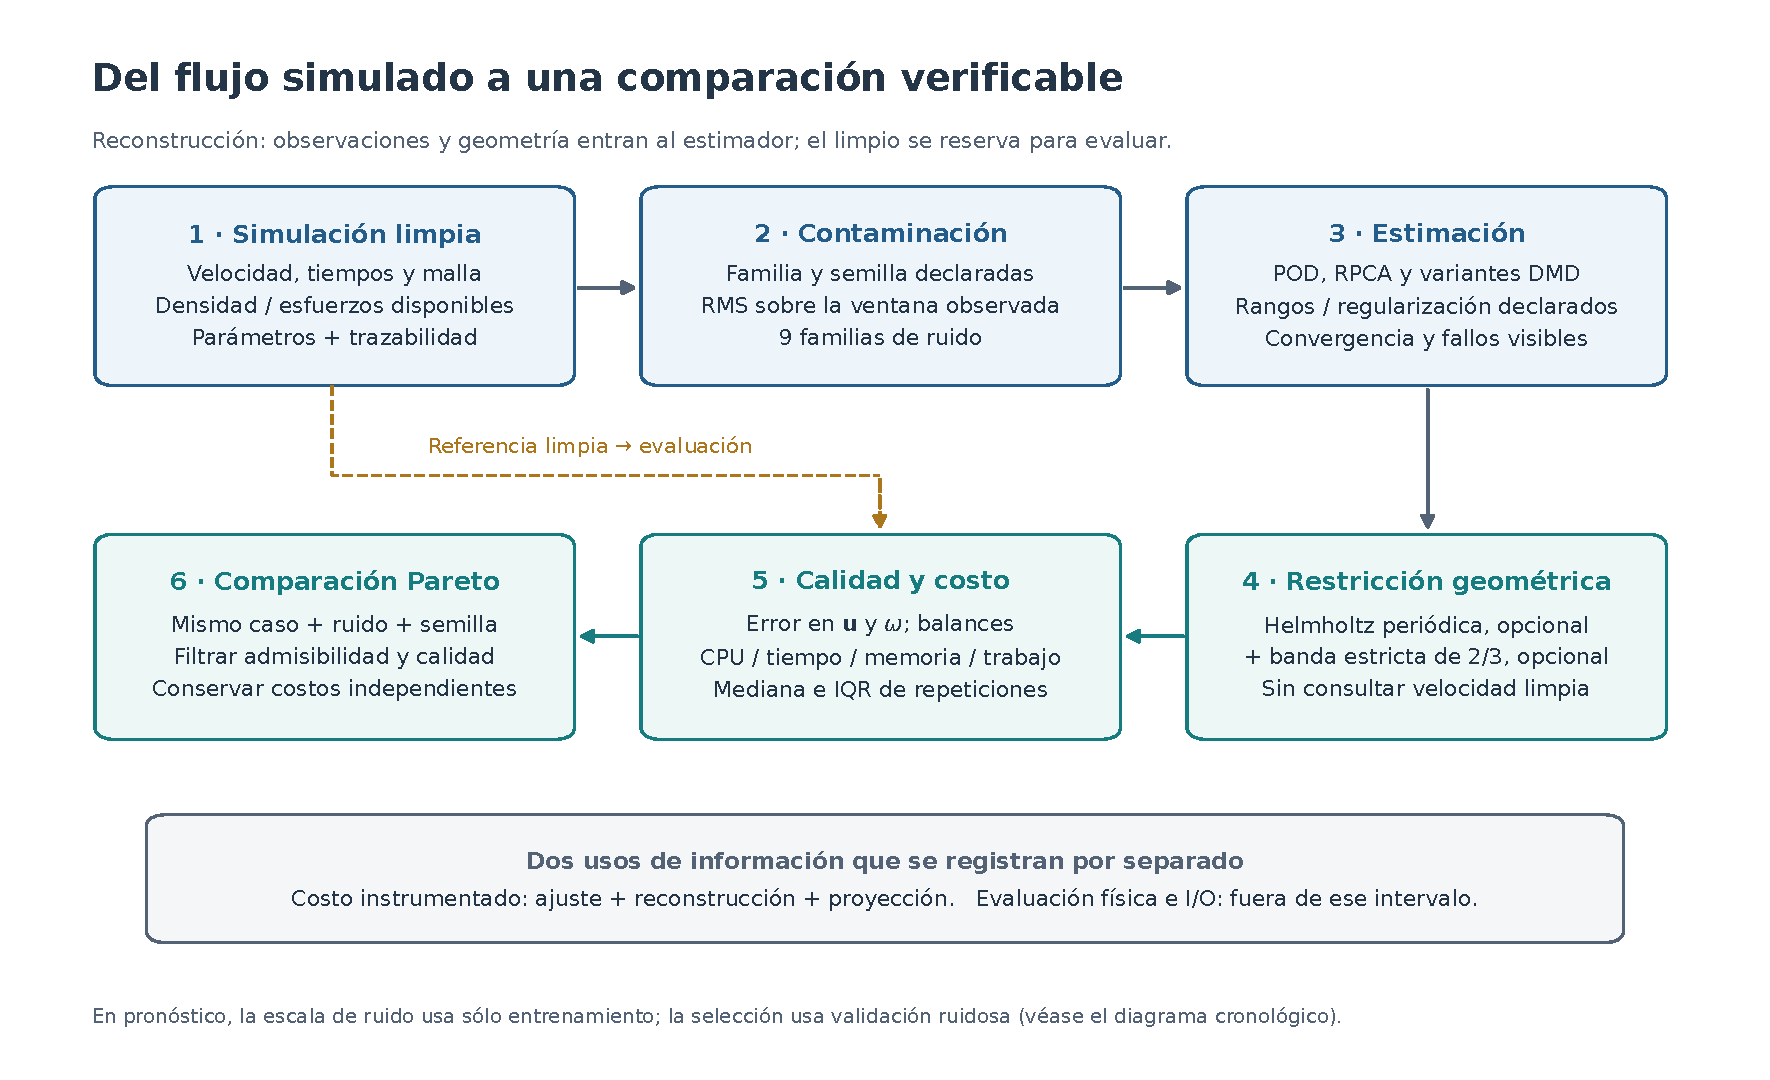
\includegraphics[width=\textwidth]{docs/research/figures/diagram_research_pipeline.pdf}
\caption{Flujo de trabajo de simulación, observación, estimación y evaluación. La referencia limpia sustenta la comparación física; la elección predictiva utiliza validación ruidosa. La frontera de recursos se interpreta junto con tolerancias y convergencia.}
\label{fig:research-pipeline}\end{figure}

\section{Verificación y trazabilidad}
Se verifica el solver frente a soluciones exactas, límites constitutivos,
residuos y refinamiento; las comprobaciones y sus configuraciones forman
parte de los artefactos. Un residuo algebraico pequeño en Euler implícito
no equivale a error de discretización pequeño. Taylor--Green de un modo
no sustituye refinamiento no lineal; una máscara de cilindro no sustituye
una geometría convergida de esfuerzos y fronteras.

Los hashes de fuentes y configuración acompañan los artefactos del baseline y corresponden a aquella ejecución; no verifican automáticamente el código integrado de fase 8. Cada campaña nueva registra su propia procedencia. La matriz observada y los parámetros quedan identificados por caso,
distribución, semilla y método. El runner registra fallos, convergencia,
configuración y recursos por réplica; produce tablas crudas y resúmenes
derivados. No se eligen hiperparámetros con el campo limpio. Las cifras
de resultados deben enlazar estos artefactos y distinguir reconstrucción
in-sample de cualquier análisis futuro fuera de muestra.

\chapter{Resultados y discusión}
\label{chap:results}
El contenido numérico de este capítulo se genera a partir de la campaña
y de sus archivos de validación. Las comparaciones se restringen a los
casos, intensidad, configuraciones y resoluciones efectivamente
registrados. Los conteos previstos del capítulo anterior no sustituyen
los conteos observados; los fallos y las condiciones que no satisfacen
los criterios permanecen visibles.

\section{Resultados calculados}
La campaña ejecutó 2808 condiciones y 8424 ajustes. Hubo 0 ajustes fallidos y 6 condiciones sin convergencia completa. Cumplieron convergencia declarada y umbrales físicos 430 condiciones.
{\scriptsize\setlength{\tabcolsep}{3pt}
\begin{longtable}{p{.17\textwidth}p{.16\textwidth}p{.30\textwidth}rrr}
\caption{Menor error mediano de velocidad entre estimadores convergidos en todas las semillas declaradas. AP: semillas aceptadas físicamente.}\\
\toprule Caso & Ruido & Método & $e_u$ [\%] & $e_\omega$ [\%] & AP \\\midrule\endfirsthead
\toprule Caso & Ruido & Método & $e_u$ [\%] & $e_\omega$ [\%] & AP \\\midrule\endhead
taylor\_\allowbreak green & gaussiano & tls\_\allowbreak dmd\_\allowbreak helmholtz\_\allowbreak dealias & 1.684 & 7.143 & 3/3 \\
taylor\_\allowbreak green & impulsivo & rpca & $<0.001$ & 0.001 & 3/3 \\
taylor\_\allowbreak green & mixed & tls\_\allowbreak dmd\_\allowbreak helmholtz\_\allowbreak dealias & 1.697 & 7.463 & 3/3 \\
taylor\_\allowbreak green & spatial\_\allowbreak correlated & tls\_\allowbreak dmd\_\allowbreak helmholtz\_\allowbreak dealias & 3.126 & 5.036 & 3/3 \\
taylor\_\allowbreak green & temporal\_\allowbreak correlated & tls\_\allowbreak dmd\_\allowbreak helmholtz\_\allowbreak dealias & 6.877 & 29.209 & 0/3 \\
taylor\_\allowbreak green & column\_\allowbreak outliers & tls\_\allowbreak dmd\_\allowbreak helmholtz\_\allowbreak dealias & 1.782 & 7.417 & 3/3 \\
taylor\_\allowbreak green & student\_\allowbreak t & tls\_\allowbreak dmd\_\allowbreak helmholtz\_\allowbreak dealias & 1.706 & 7.633 & 3/3 \\
taylor\_\allowbreak green & heteroscedastic & tls\_\allowbreak dmd\_\allowbreak helmholtz\_\allowbreak dealias & 1.850 & 7.740 & 3/3 \\
taylor\_\allowbreak green & sensor\_\allowbreak drift & stable\_\allowbreak rpca & 19.429 & 4.125 & 0/3 \\
interacting\_\allowbreak vortices & gaussiano & tls\_\allowbreak dmd\_\allowbreak helmholtz\_\allowbreak dealias & 3.800 & 27.128 & 0/3 \\
interacting\_\allowbreak vortices & impulsivo & tls\_\allowbreak dmd\_\allowbreak helmholtz\_\allowbreak dealias & 3.901 & 27.574 & 0/3 \\
interacting\_\allowbreak vortices & mixed & tls\_\allowbreak dmd\_\allowbreak helmholtz\_\allowbreak dealias & 3.797 & 27.166 & 0/3 \\
interacting\_\allowbreak vortices & spatial\_\allowbreak correlated & tls\_\allowbreak dmd\_\allowbreak helmholtz\_\allowbreak dealias & 5.488 & 17.344 & 3/3 \\
interacting\_\allowbreak vortices & temporal\_\allowbreak correlated & tls\_\allowbreak dmd\_\allowbreak helmholtz\_\allowbreak dealias & 7.520 & 59.521 & 0/3 \\
interacting\_\allowbreak vortices & column\_\allowbreak outliers & rpca & 7.140 & 17.838 & 0/3 \\
interacting\_\allowbreak vortices & student\_\allowbreak t & tls\_\allowbreak dmd\_\allowbreak helmholtz\_\allowbreak dealias & 3.869 & 27.773 & 0/3 \\
interacting\_\allowbreak vortices & heteroscedastic & tls\_\allowbreak dmd\_\allowbreak helmholtz\_\allowbreak dealias & 3.834 & 27.568 & 0/3 \\
interacting\_\allowbreak vortices & sensor\_\allowbreak drift & identity\_\allowbreak helmholtz & 20.000 & $<0.001$ & 0/3 \\
decaying\_\allowbreak turbulence & gaussiano & tls\_\allowbreak dmd\_\allowbreak helmholtz\_\allowbreak dealias & 3.985 & 17.705 & 3/3 \\
decaying\_\allowbreak turbulence & impulsivo & rpca & 2.174 & 5.805 & 3/3 \\
decaying\_\allowbreak turbulence & mixed & tls\_\allowbreak dmd\_\allowbreak helmholtz\_\allowbreak dealias & 3.999 & 17.746 & 3/3 \\
decaying\_\allowbreak turbulence & spatial\_\allowbreak correlated & tls\_\allowbreak dmd\_\allowbreak helmholtz\_\allowbreak dealias & 5.754 & 10.801 & 3/3 \\
decaying\_\allowbreak turbulence & temporal\_\allowbreak correlated & tls\_\allowbreak dmd\_\allowbreak helmholtz\_\allowbreak dealias & 7.875 & 37.529 & 0/3 \\
decaying\_\allowbreak turbulence & column\_\allowbreak outliers & rpca & 5.056 & 8.473 & 3/3 \\
decaying\_\allowbreak turbulence & student\_\allowbreak t & tls\_\allowbreak dmd\_\allowbreak helmholtz\_\allowbreak dealias & 4.018 & 17.813 & 3/3 \\
decaying\_\allowbreak turbulence & heteroscedastic & tls\_\allowbreak dmd\_\allowbreak helmholtz\_\allowbreak dealias & 4.414 & 19.128 & 3/3 \\
decaying\_\allowbreak turbulence & sensor\_\allowbreak drift & rpca & 19.968 & 3.069 & 0/3 \\
oldroyd\_\allowbreak b\_\allowbreak 2d & gaussiano & tls\_\allowbreak dmd\_\allowbreak helmholtz\_\allowbreak dealias & 2.768 & 13.333 & 3/3 \\
oldroyd\_\allowbreak b\_\allowbreak 2d & impulsivo & rpca & 0.995 & 2.721 & 3/3 \\
oldroyd\_\allowbreak b\_\allowbreak 2d & mixed & tls\_\allowbreak dmd\_\allowbreak helmholtz\_\allowbreak dealias & 2.799 & 13.078 & 3/3 \\
oldroyd\_\allowbreak b\_\allowbreak 2d & spatial\_\allowbreak correlated & tls\_\allowbreak dmd\_\allowbreak helmholtz\_\allowbreak dealias & 4.203 & 8.810 & 3/3 \\
oldroyd\_\allowbreak b\_\allowbreak 2d & temporal\_\allowbreak correlated & tls\_\allowbreak dmd\_\allowbreak helmholtz\_\allowbreak dealias & 7.408 & 39.902 & 0/3 \\
oldroyd\_\allowbreak b\_\allowbreak 2d & column\_\allowbreak outliers & rpca & 4.010 & 6.436 & 3/3 \\
oldroyd\_\allowbreak b\_\allowbreak 2d & student\_\allowbreak t & tls\_\allowbreak dmd\_\allowbreak helmholtz\_\allowbreak dealias & 2.774 & 12.769 & 3/3 \\
oldroyd\_\allowbreak b\_\allowbreak 2d & heteroscedastic & tls\_\allowbreak dmd\_\allowbreak helmholtz\_\allowbreak dealias & 2.741 & 12.751 & 3/3 \\
oldroyd\_\allowbreak b\_\allowbreak 2d & sensor\_\allowbreak drift & stable\_\allowbreak rpca & 19.791 & 8.187 & 0/3 \\
fene\_\allowbreak p\_\allowbreak 2d & gaussiano & tls\_\allowbreak dmd\_\allowbreak helmholtz\_\allowbreak dealias & 2.770 & 13.337 & 3/3 \\
fene\_\allowbreak p\_\allowbreak 2d & impulsivo & rpca & 0.994 & 2.720 & 3/3 \\
fene\_\allowbreak p\_\allowbreak 2d & mixed & tls\_\allowbreak dmd\_\allowbreak helmholtz\_\allowbreak dealias & 2.801 & 13.082 & 3/3 \\
fene\_\allowbreak p\_\allowbreak 2d & spatial\_\allowbreak correlated & tls\_\allowbreak dmd\_\allowbreak helmholtz\_\allowbreak dealias & 4.204 & 8.815 & 3/3 \\
fene\_\allowbreak p\_\allowbreak 2d & temporal\_\allowbreak correlated & tls\_\allowbreak dmd\_\allowbreak helmholtz\_\allowbreak dealias & 7.408 & 39.908 & 0/3 \\
fene\_\allowbreak p\_\allowbreak 2d & column\_\allowbreak outliers & rpca & 4.009 & 6.438 & 3/3 \\
fene\_\allowbreak p\_\allowbreak 2d & student\_\allowbreak t & tls\_\allowbreak dmd\_\allowbreak helmholtz\_\allowbreak dealias & 2.777 & 12.772 & 3/3 \\
fene\_\allowbreak p\_\allowbreak 2d & heteroscedastic & tls\_\allowbreak dmd\_\allowbreak helmholtz\_\allowbreak dealias & 2.743 & 12.754 & 3/3 \\
fene\_\allowbreak p\_\allowbreak 2d & sensor\_\allowbreak drift & stable\_\allowbreak rpca & 19.791 & 8.191 & 0/3 \\
hb\_\allowbreak thinning\_\allowbreak 2d & gaussiano & tls\_\allowbreak dmd\_\allowbreak helmholtz\_\allowbreak dealias & 4.197 & 18.286 & 3/3 \\
hb\_\allowbreak thinning\_\allowbreak 2d & impulsivo & tls\_\allowbreak dmd\_\allowbreak helmholtz\_\allowbreak dealias & 4.183 & 18.512 & 3/3 \\
hb\_\allowbreak thinning\_\allowbreak 2d & mixed & tls\_\allowbreak dmd\_\allowbreak helmholtz\_\allowbreak dealias & 4.236 & 18.728 & 3/3 \\
hb\_\allowbreak thinning\_\allowbreak 2d & spatial\_\allowbreak correlated & tls\_\allowbreak dmd\_\allowbreak helmholtz\_\allowbreak dealias & 5.914 & 13.865 & 3/3 \\
hb\_\allowbreak thinning\_\allowbreak 2d & temporal\_\allowbreak correlated & tls\_\allowbreak dmd\_\allowbreak helmholtz\_\allowbreak dealias & 7.712 & 40.167 & 0/3 \\
hb\_\allowbreak thinning\_\allowbreak 2d & column\_\allowbreak outliers & rpca & 6.085 & 13.029 & 3/3 \\
hb\_\allowbreak thinning\_\allowbreak 2d & student\_\allowbreak t & tls\_\allowbreak dmd\_\allowbreak helmholtz\_\allowbreak dealias & 4.208 & 18.513 & 3/3 \\
hb\_\allowbreak thinning\_\allowbreak 2d & heteroscedastic & tls\_\allowbreak dmd\_\allowbreak helmholtz\_\allowbreak dealias & 4.213 & 18.594 & 3/3 \\
hb\_\allowbreak thinning\_\allowbreak 2d & sensor\_\allowbreak drift & rpca & 19.992 & 9.545 & 0/3 \\
bingham\_\allowbreak 2d & gaussiano & tls\_\allowbreak dmd\_\allowbreak helmholtz\_\allowbreak dealias & 4.010 & 18.135 & 3/3 \\
bingham\_\allowbreak 2d & impulsivo & tls\_\allowbreak dmd\_\allowbreak helmholtz\_\allowbreak dealias & 3.999 & 18.409 & 3/3 \\
bingham\_\allowbreak 2d & mixed & tls\_\allowbreak dmd\_\allowbreak helmholtz\_\allowbreak dealias & 4.048 & 18.591 & 3/3 \\
bingham\_\allowbreak 2d & spatial\_\allowbreak correlated & tls\_\allowbreak dmd\_\allowbreak helmholtz\_\allowbreak dealias & 5.813 & 13.482 & 3/3 \\
bingham\_\allowbreak 2d & temporal\_\allowbreak correlated & tls\_\allowbreak dmd\_\allowbreak helmholtz\_\allowbreak dealias & 7.613 & 40.576 & 0/3 \\
bingham\_\allowbreak 2d & column\_\allowbreak outliers & rpca & 5.851 & 12.486 & 3/3 \\
bingham\_\allowbreak 2d & student\_\allowbreak t & tls\_\allowbreak dmd\_\allowbreak helmholtz\_\allowbreak dealias & 4.021 & 18.405 & 3/3 \\
bingham\_\allowbreak 2d & heteroscedastic & tls\_\allowbreak dmd\_\allowbreak helmholtz\_\allowbreak dealias & 4.032 & 18.494 & 3/3 \\
bingham\_\allowbreak 2d & sensor\_\allowbreak drift & rpca & 19.962 & 8.933 & 0/3 \\
hb\_\allowbreak thickening\_\allowbreak 2d & gaussiano & tls\_\allowbreak dmd\_\allowbreak helmholtz\_\allowbreak dealias & 3.810 & 18.074 & 3/3 \\
hb\_\allowbreak thickening\_\allowbreak 2d & impulsivo & tls\_\allowbreak dmd\_\allowbreak helmholtz\_\allowbreak dealias & 3.804 & 18.384 & 3/3 \\
hb\_\allowbreak thickening\_\allowbreak 2d & mixed & tls\_\allowbreak dmd\_\allowbreak helmholtz\_\allowbreak dealias & 3.848 & 18.538 & 3/3 \\
hb\_\allowbreak thickening\_\allowbreak 2d & spatial\_\allowbreak correlated & tls\_\allowbreak dmd\_\allowbreak helmholtz\_\allowbreak dealias & 5.706 & 13.174 & 3/3 \\
hb\_\allowbreak thickening\_\allowbreak 2d & temporal\_\allowbreak correlated & tls\_\allowbreak dmd\_\allowbreak helmholtz\_\allowbreak dealias & 7.507 & 41.080 & 0/3 \\
hb\_\allowbreak thickening\_\allowbreak 2d & column\_\allowbreak outliers & rpca & 5.587 & 11.931 & 3/3 \\
hb\_\allowbreak thickening\_\allowbreak 2d & student\_\allowbreak t & tls\_\allowbreak dmd\_\allowbreak helmholtz\_\allowbreak dealias & 3.822 & 18.395 & 3/3 \\
hb\_\allowbreak thickening\_\allowbreak 2d & heteroscedastic & tls\_\allowbreak dmd\_\allowbreak helmholtz\_\allowbreak dealias & 3.846 & 18.520 & 3/3 \\
hb\_\allowbreak thickening\_\allowbreak 2d & sensor\_\allowbreak drift & rpca & 19.947 & 8.377 & 0/3 \\
\bottomrule\end{longtable}}
Sólo 150 de 216 grupos caso/ruido/semilla tienen algún estimador admisible a estos umbrales. Los 66 restantes no ofrecen solución al costo y fidelidad fijados. Los valores pequeños se indican mediante desigualdad para no representar una aproximación como error exactamente cero. Estos conteos son descriptivos del banco y no probabilidades de éxito en mediciones reales.
\begin{figure}[htbp]\centering
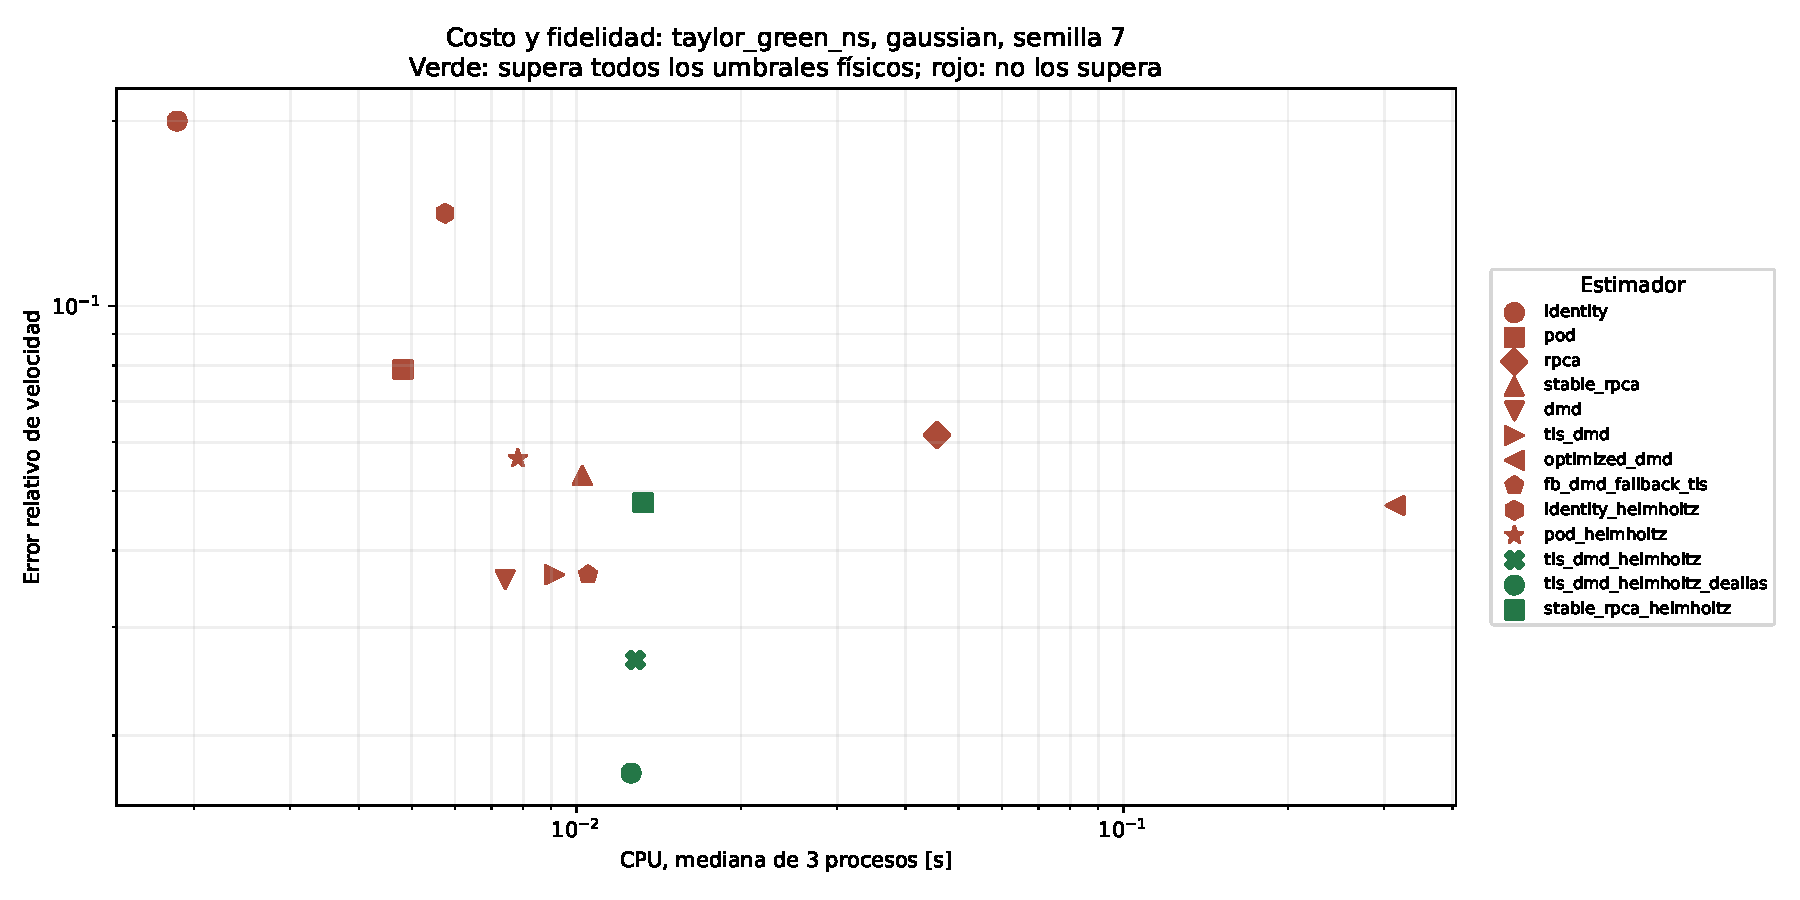
\includegraphics[width=.95\textwidth]{results/research/extended_physics_2026-10-14/figures/cost_quality.pdf}
\caption{Costo medido y error de velocidad en una condición coincidente. La aceptación incluye vorticidad, divergencia y energía; en canales, paredes.}\end{figure}
\section{Límites de la inferencia}
Las semillas son réplicas de contaminación del mismo campo; las repeticiones de recursos no aumentan el tamaño de muestra de calidad. La evaluación es reconstrucción dentro de la ventana, sin pronóstico ni mediciones PIV reales. El parámetro de ruido conocido es información del experimento sintético. Los perfiles HB estacionarios favorecen bajo rango temporal y no representan estelas; consulte los metadatos para distinguir perfiles de canales y solvers bidimensionales. La reconstrucción de velocidad no estima densidad: las métricas de masa y energía requieren densidad declarada. Los tiempos y métricas históricas de magnitud de velocidad no son directamente comparables a estas componentes vectoriales ni al entorno instrumentado.
Los CSV, ledger JSONL, configuraciones y hashes acompañan esta discusión en \texttt{results/research/extended\_\allowbreak physics\_\allowbreak 2026-10-14}. Las figuras de todos los casos se exportan a PNG y PDF; el resumen distingue convergencia y factibilidad física.

\section{Hallazgos de la ampliación y controles}
En Taylor--Green gaussiano, TLS-DMD de rango cuatro pasa de 3.709\% a 1.684\% de error mediano de velocidad con proyección y banda declarada. En los tres casos newtonianos gaussianos, las condiciones aceptadas son 0 sin proyección y 12 con proyección. No se ajustó la banda utilizando la referencia limpia.
El dispatcher forward--backward a TLS utilizó su alternativa predeclarada en 23 condiciones. Los fallos primarios permanecen en los registros y su trabajo cuenta en el costo total.
\section{Pronóstico cronológico ejecutado}
Se evaluaron 60 condiciones con cinco campos, cuatro modelos de contaminación y tres semillas. Cada condición considera 29 opciones, con ajuste sólo en entrenamiento, selección por error de validación ruidosa y evaluación final en un bloque futuro independiente. Las opciones físicas comparten ajustes; no se cuentan como entrenamientos independientes.
La opción seleccionada mejora persistencia sin filtrar en 48 condiciones y persistencia filtrada en 43. Se exige una diferencia absoluta mayor que $10^{-10}$ en el error relativo de velocidad; las diferencias de redondeo se consideran empates. Estos conteos son condicionales al banco y no probabilidades de éxito en mediciones reales.
\begin{figure}[htbp]\centering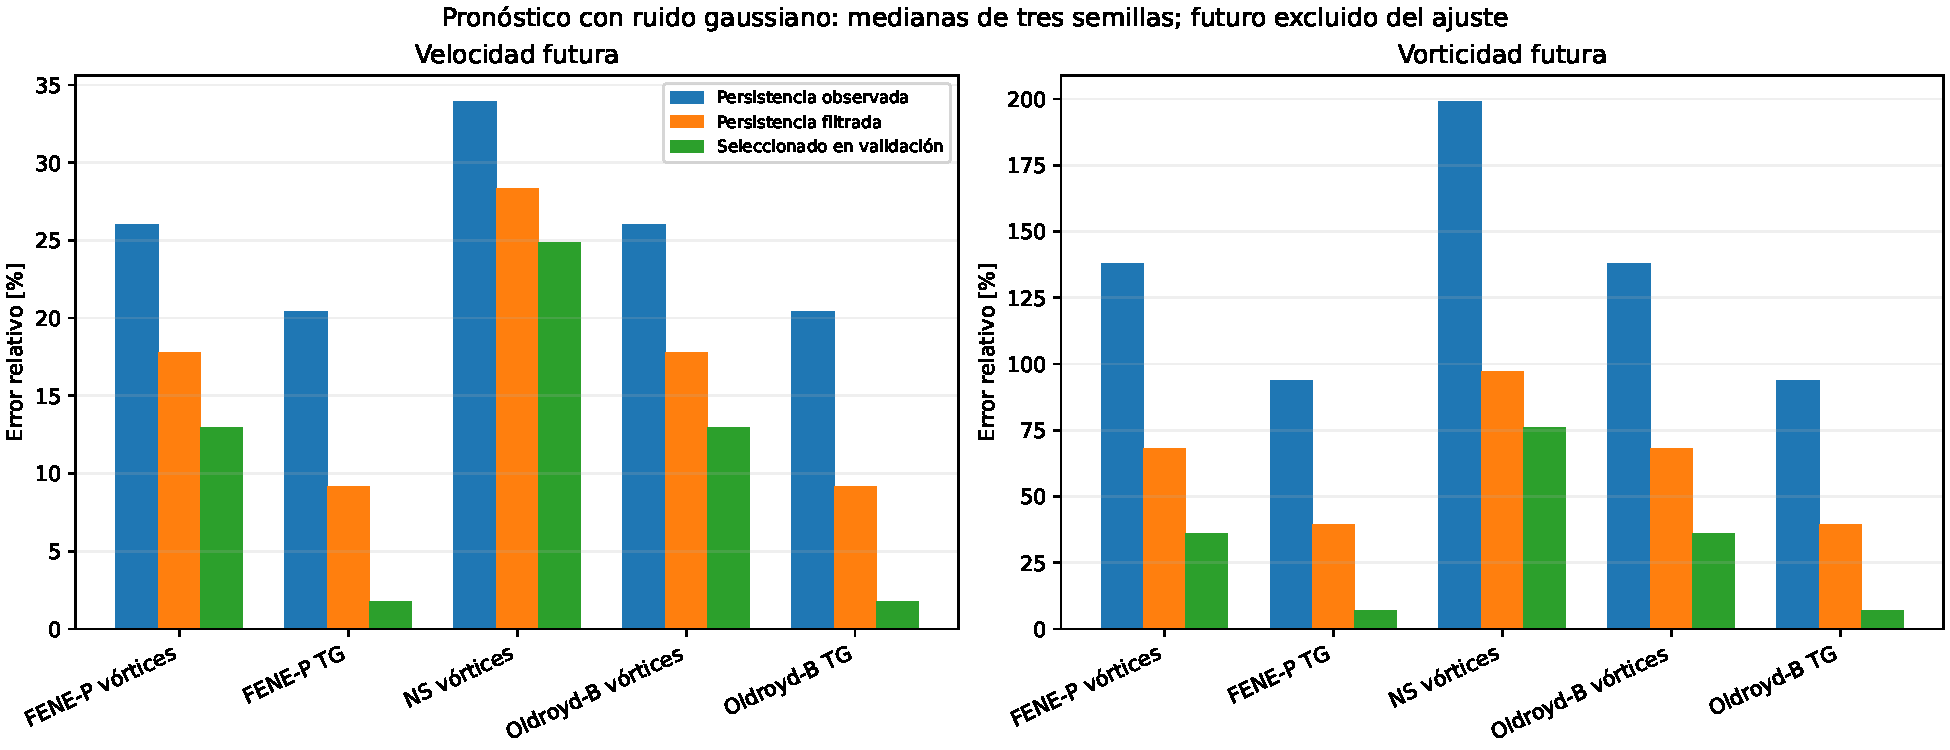
\includegraphics[width=\textwidth]{results/research/forecasting_extended_2026-10-14/figures/holdout_comparison.pdf}
\caption{Errores en el futuro excluido del ajuste. Comparar con persistencia filtrada evita atribuir toda mejora al modelo dinámico.}\end{figure}
\section{Banco reológico con condiciones iniciales comunes}
Seis fluidos comparten velocidad inicial, densidad, dominio, malla y tiempos. Las diferencias numéricas representan cambios constitutivos; no son errores de reconstrucción. Las viscosidades HB se igualan en la tasa de corte declarada y las constantes viscoelásticas se comparan en su normalización nominal. La cercanía Oldroyd-B/FENE-P observada no demuestra capacidad de identificar materiales con velocidad ruidosa.
\begin{figure}[htbp]\centering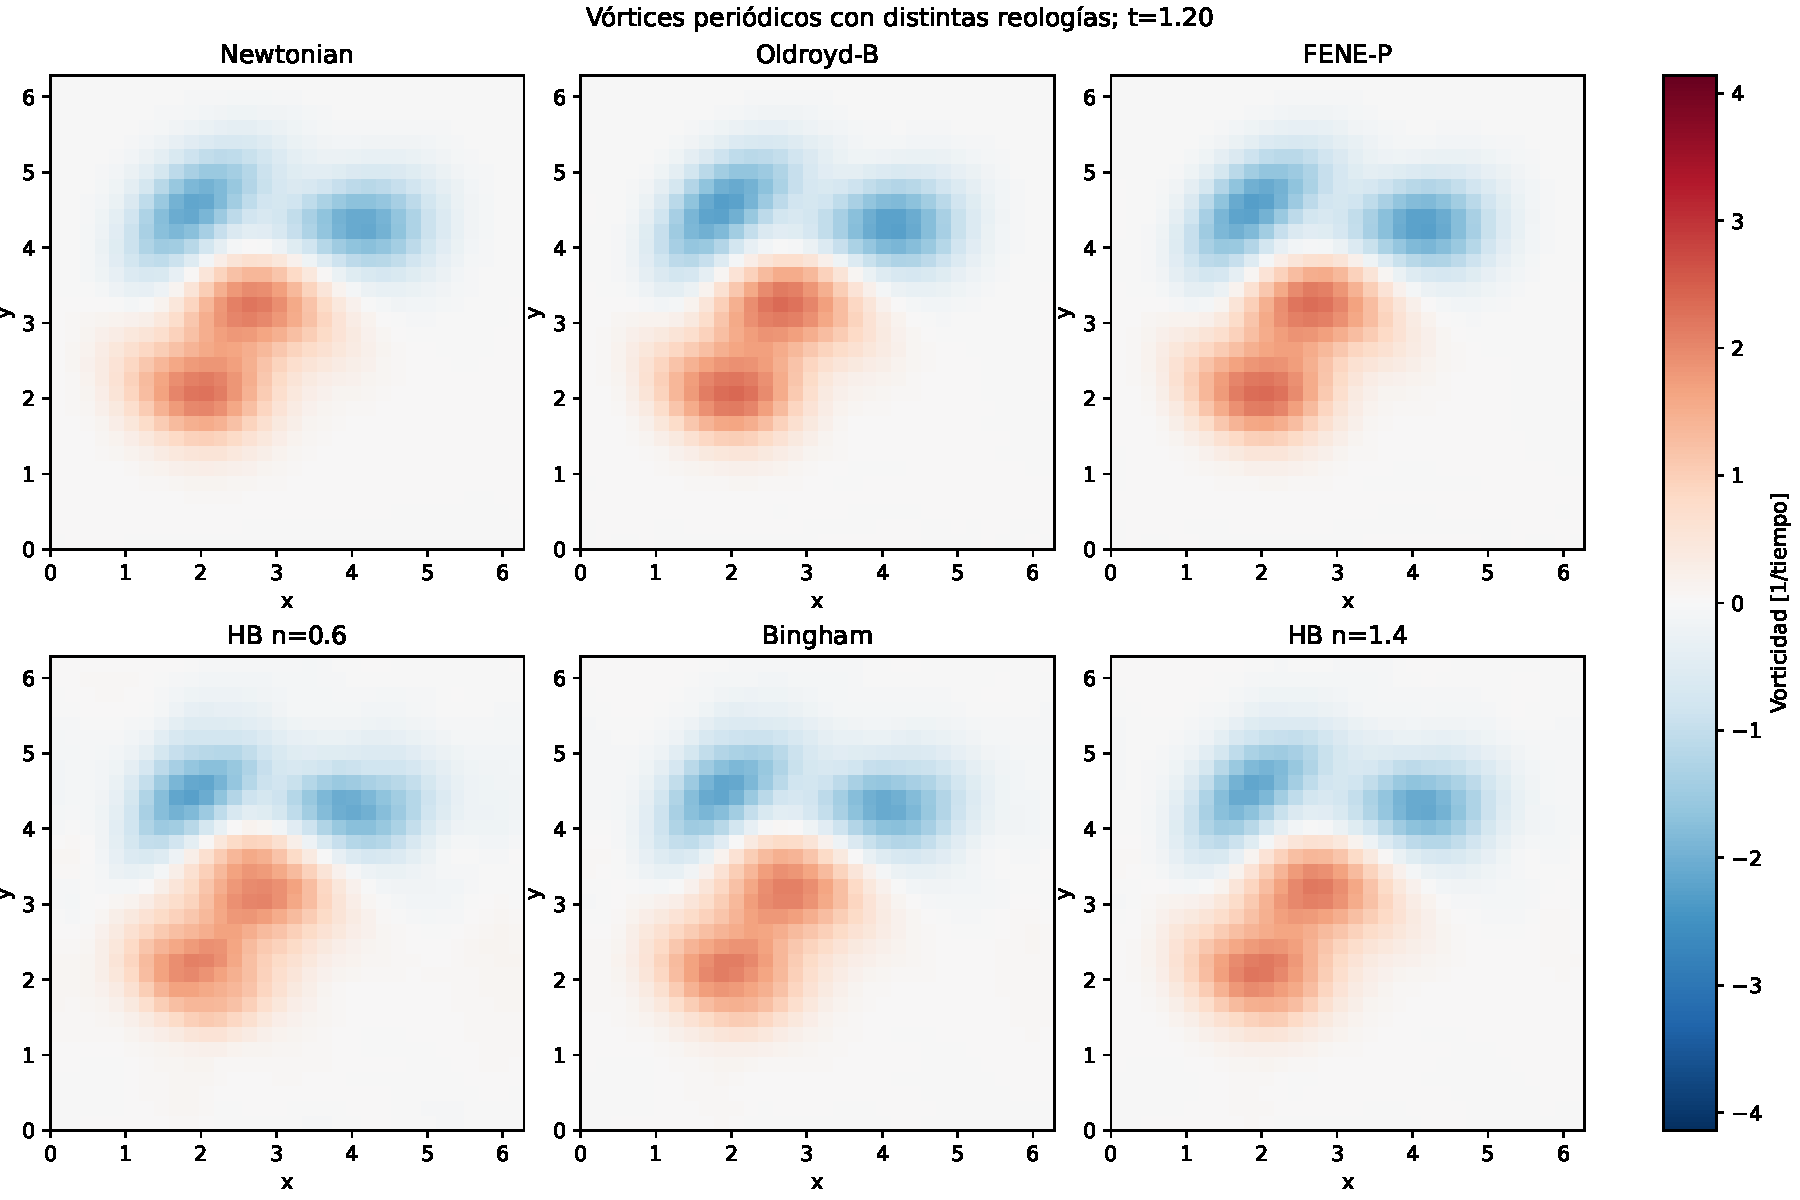
\includegraphics[width=\textwidth]{results/research/rheology_matched_2026-10-14/final_vorticity.pdf}
\caption{Vorticidad final de seis modelos sobre el mismo estado inicial periódico. Las diferencias dependen de la ley constitutiva y su normalización declarada.}\end{figure}
\section{Cuestiones todavía abiertas}
La vorticidad futura en casos de vórtices conserva errores importantes, y ninguna condición de ruido temporal o deriva de sensor satisface los umbrales de reconstrucción. La proyección reduce divergencia pero no recupera por sí sola sesgo de sensor, esfuerzos o memoria constitutiva. Los wakes externos, EVP, 3D, PIV, GPU y aprendizaje profundo siguen pendientes de ejecución.

% Generated by python/scripts/build_highres_chapter.py; do not edit.
\clearpage
\section{Mallas ampliadas y evolución física}
\label{sec:highres}
Esta ampliación responde a la representatividad de las mallas y permite observar la evolución de los campos. Se integran de nuevo las ecuaciones en mallas mayores: los mapas mostrados proceden de los arrays calculados, sin generar ni completar estructuras mediante ilustración. La interpolación periódica de Fourier se utiliza únicamente para comparar soluciones calculadas por separado. Las campañas anteriores conservan sus resultados y se distinguen de las nuevas condiciones, viscosidades y horizontes.

El corpus completo contiene 8 integraciones espaciales newtonianas, 4 controles temporales newtonianos y 6 controles analíticos; 9 configuraciones viscoelásticas/control newtoniano; 18 configuraciones viscoplásticas; y 60 condiciones adicionales de reconstrucción. Un control analítico no equivale a un nuevo flujo no lineal ni a un ajuste de reconstrucción. Un seguimiento exploratorio posterior añade 24 condiciones con ancho de banda físico fijo; conserva el resultado inicial y se presenta por separado.

\begingroup\small\setlength{\tabcolsep}{3pt}
\begin{longtable}{@{}>{\raggedright\arraybackslash}p{4.3cm}>{\raggedright\arraybackslash}p{4.6cm}>{\raggedright\arraybackslash}p{2.6cm}>{\raggedright\arraybackslash}p{3.5cm}@{}}
\caption{Integraciones efectivamente ejecutadas y tiempos adimensionales; las campañas tienen horizontes diferentes.}\\
\toprule
Banco & Mallas calculadas & Horizonte & Estados por ejecución \\
\midrule\endfirsthead
\toprule
Banco & Mallas calculadas & Horizonte & Estados por ejecución \\
\midrule\endhead
Navier–Stokes 2D & 64$^2$, 128$^2$, 256$^2$, 512$^2$ & 0–4 & 41 \\
Oldroyd-B y FENE-P & 64$^2$, 128$^2$, 256$^2$ & 0–2.4 & 25 \\
HB/Bingham, evolución & 64$^2$, 128$^2$ & 0–2 & 21 \\
HB/Bingham, referencia corta & 256$^2$ & 0–0.1 & 2 \\
Reconstrucción de cuatro vórtices & 128$^2$, 256$^2$ & 0–4 & 41 \\
\bottomrule\end{longtable}\endgroup

\clearpage
\subsection{\texorpdfstring{Qué representa una malla: error completo, tiempo y espectro}{Qué representa una malla: error completo, tiempo y espectro}}
La resolución se juzga contra una ejecución fina del mismo solver, que sigue siendo una referencia numérica. El error en modos comunes compara solamente las escalas compartidas. El error completo de una cantidad $q$ es \[ e_q^{\mathrm{completo}}(t)=\frac{\norm{\mathcal{I}_{N\to N_f}q_N(t)-q_{N_f}(t)}_2}{\norm{q_{N_f}(t)}_2},\qquad e_{q,\max}=\max_{t\in\mathcal{T}_{\mathrm{guardada}}}e_q^{\mathrm{completo}}(t).\] La prolongación periódica $\mathcal{I}$ sólo transfiere campos calculados por separado y la referencia completa no se filtra. Así se contabilizan las estructuras que la malla gruesa omite. Las tablas usan el máximo entre todos los instantes guardados, no el promedio ni solamente el estado final.

El núcleo gaussiano inicial tiene ancho $\sigma=0.065L$, con $L=2\pi$: las mallas $64^2$, $128^2$, $256^2$ y $512^2$ proporcionan 4.16, 8.32, 16.64 y 33.28 celdas por $\sigma$. El estado aleatorio inicial newtoniano tiene corte Fourier 8, con 8, 16, 32 y 64 celdas por su menor longitud de onda inicial. Estas cifras describen el estado inicial; los gradientes posteriores requieren sus propios controles. El criterio exploratorio newtoniano exige errores máximos de velocidad y vorticidad menores al $1\,\%$, además de cola de enstrofía por componente menor que $10^{-4}$. Es un diagnóstico de estas condiciones, sin presentarlo como preregistro ciego ni certificado universal de DNS.

Las imágenes mantienen dominio y escalas de color por magnitud dentro de cada comparación. Los bordes opuestos son vecinos periódicos: un vórtice que sale por un borde reaparece por el opuesto. Las flechas y líneas de corriente describen el campo instantáneo, no trayectorias de partículas. Los mapas de error tienen barras propias; el error cero de una referencia frente a sí misma no demuestra exactitud física. Los registros de CPU y tiempo se conservan, pero las ejecuciones compartieron el equipo y sus alcances de medición difieren; no sustentan una comparación precisa de velocidad entre solvers.

\clearpage
\subsection{\texorpdfstring{Navier–Stokes: interacción, espectros y referencia 512$^2$}{Navier–Stokes: interacción, espectros y referencia 512 por 512}}
Se estudiaron dos estados no lineales periódicos con $\nu$=0.01, velocidad RMS inicial U=0.8, semilla 17 y horizonte T=4. El número de Reynolds basado en L=2$\pi$ es 502.7; para el ancho del núcleo es 32.67. Son escalas declaradas, no una clasificación universal del régimen. El nombre del caso «turbulencia en decaimiento» no acredita caos; no se calcula un exponente de Lyapunov.

\begingroup\small\setlength{\tabcolsep}{3pt}
\begin{longtable}{@{}>{\raggedright\arraybackslash}p{3.9588cm}>{\raggedright\arraybackslash}p{1.3856cm}>{\raggedright\arraybackslash}p{1.5835cm}>{\raggedright\arraybackslash}p{2.4743cm}>{\raggedright\arraybackslash}p{2.4743cm}>{\raggedright\arraybackslash}p{2.9691cm}@{}}
\caption{Errores completos máximos sobre los 41 estados; incluye las escalas no representadas.}\\
\toprule
Flujo & Malla & Referencia & Máx. error u & Máx. error $\omega$ & Criterio exploratorio \\
\midrule\endfirsthead
\toprule
Flujo & Malla & Referencia & Máx. error u & Máx. error $\omega$ & Criterio exploratorio \\
\midrule\endhead
Cuatro vórtices en interacción & 64$^2$ & 512$^2$ & 0.02337 \% & 0.3626 \% & Sí \\
Cuatro vórtices en interacción & 128$^2$ & 512$^2$ & 2.471e-05 \% & 7.410e-04 \% & Sí \\
Cuatro vórtices en interacción & 256$^2$ & 512$^2$ & 4.027e-08 \% & 2.671e-07 \% & Sí \\
Turbulencia 2D en decaimiento & 64$^2$ & 512$^2$ & 0.2007 \% & 1.312 \% & No \\
Turbulencia 2D en decaimiento & 128$^2$ & 512$^2$ & 0.002455 \% & 0.03032 \% & Sí \\
Turbulencia 2D en decaimiento & 256$^2$ & 512$^2$ & 7.525e-08 \% & 1.565e-06 \% & Sí \\
\bottomrule\end{longtable}\endgroup

Para cuatro vórtices, 64$^2$ ya presenta un máximo de vorticidad de 0.3626 \% frente a 512$^2$ y cumple el diagnóstico de este caso suave. En cambio, el estado en decaimiento da 1.312 \% en 64$^2$ y 0.03032 \% en 128$^2$. El primero falla el nivel del 1 \% y la cola espectral exigida. La representatividad depende del flujo y de la cantidad observada; no basta extrapolar la convergencia de un estado a todo el banco.

\clearpage
\begin{landscape}
\begin{figure}[p]\centering
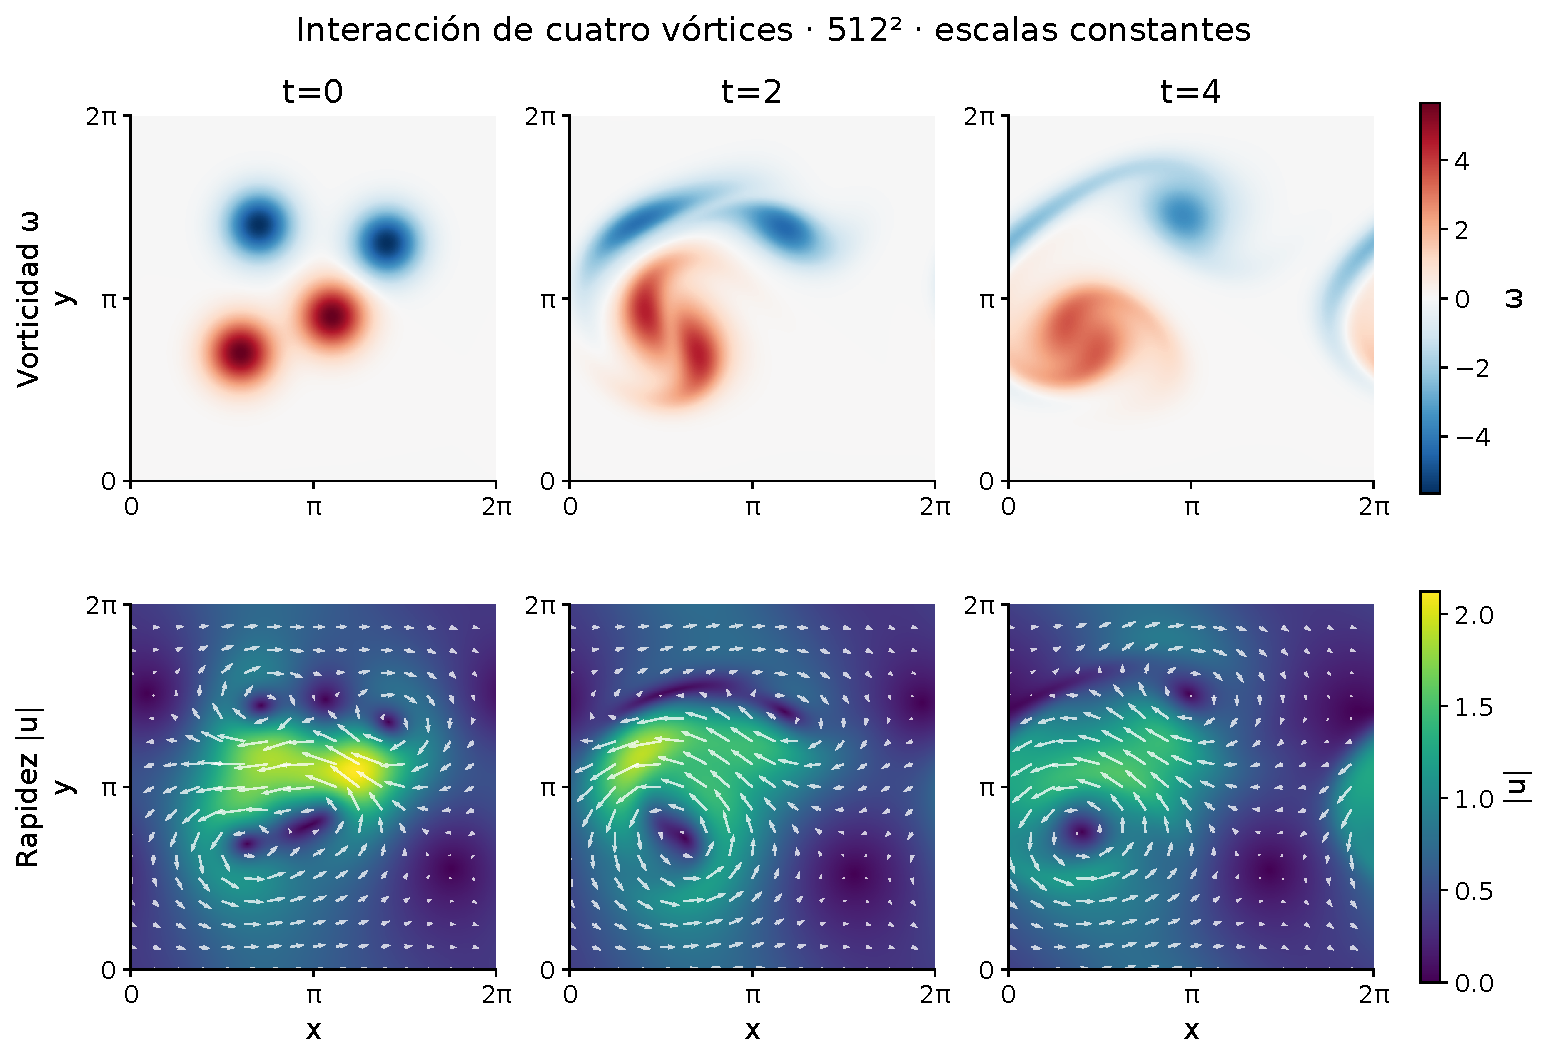
\includegraphics[width=\linewidth,height=.80\textwidth,keepaspectratio]{results/research/highres_newtonian_2026-10-14/figures/interacting_vortices_evolution_publication.pdf}
\caption{Cuatro vórtices en interacción en 512$^2$: tres estados calculados en t=0, t=2 y t=4. Vorticidad con signo y rapidez usan escalas constantes por fila; las flechas muestran velocidad instantánea. Se observan deformación e intercambio de estructura en un dominio periódico, no una estela externa. La secuencia original de cinco tiempos y la animación completa quedan enlazadas como compañeros.}
\label{fig:interacting_vortices-evolution}\end{figure}
\end{landscape}
\clearpage
\clearpage
\begin{landscape}
\begin{figure}[p]\centering
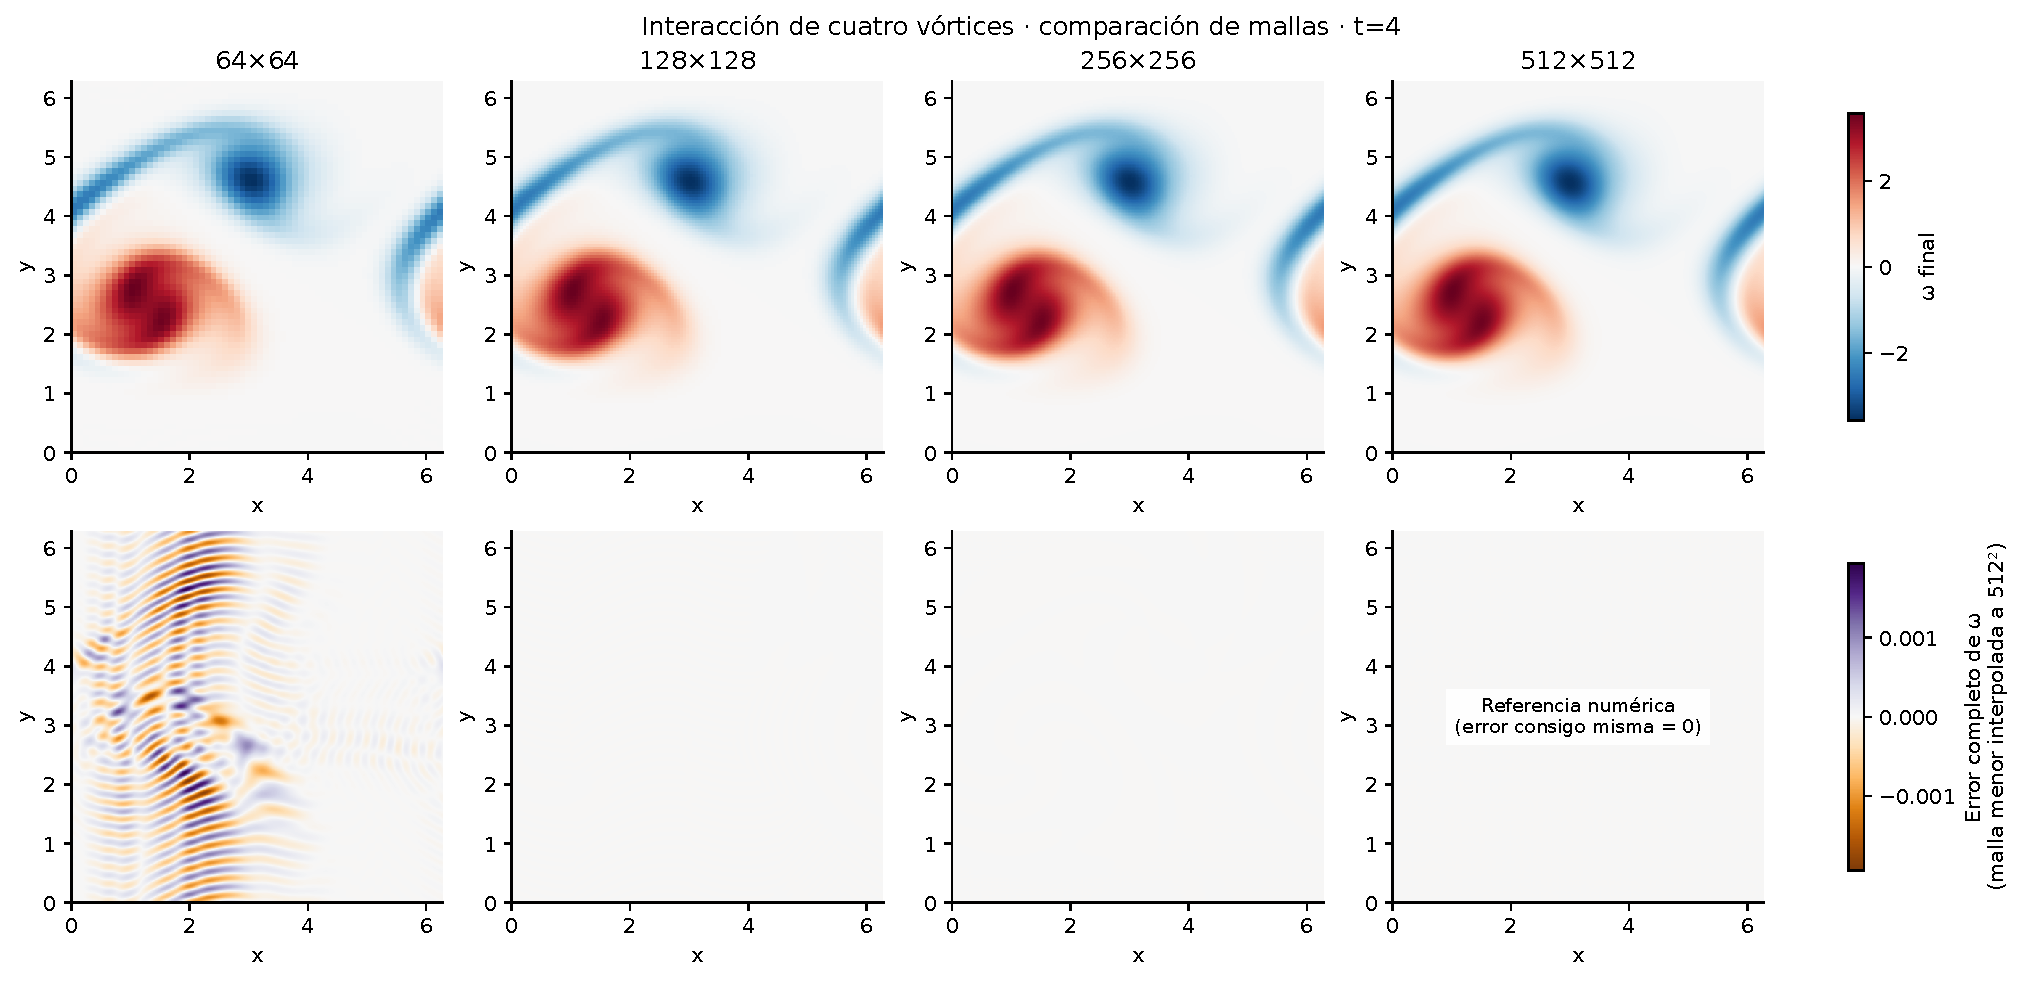
\includegraphics[width=\linewidth,height=.80\textwidth,keepaspectratio]{results/research/highres_newtonian_2026-10-14/figures/interacting_vortices_grid_comparison.pdf}
\caption{Cuatro vórtices en interacción: vorticidad final calculada en cuatro mallas y diferencias de campo completo respecto a 512$^2$. La fila inferior transfiere cada solución gruesa a la malla fina; su barra de error es distinta de la barra física. El panel 512$^2$ se compara consigo mismo y tiene error cero por definición.}
\label{fig:interacting_vortices-grids}\end{figure}
\end{landscape}
\clearpage
\clearpage
\begin{figure}[p]\centering
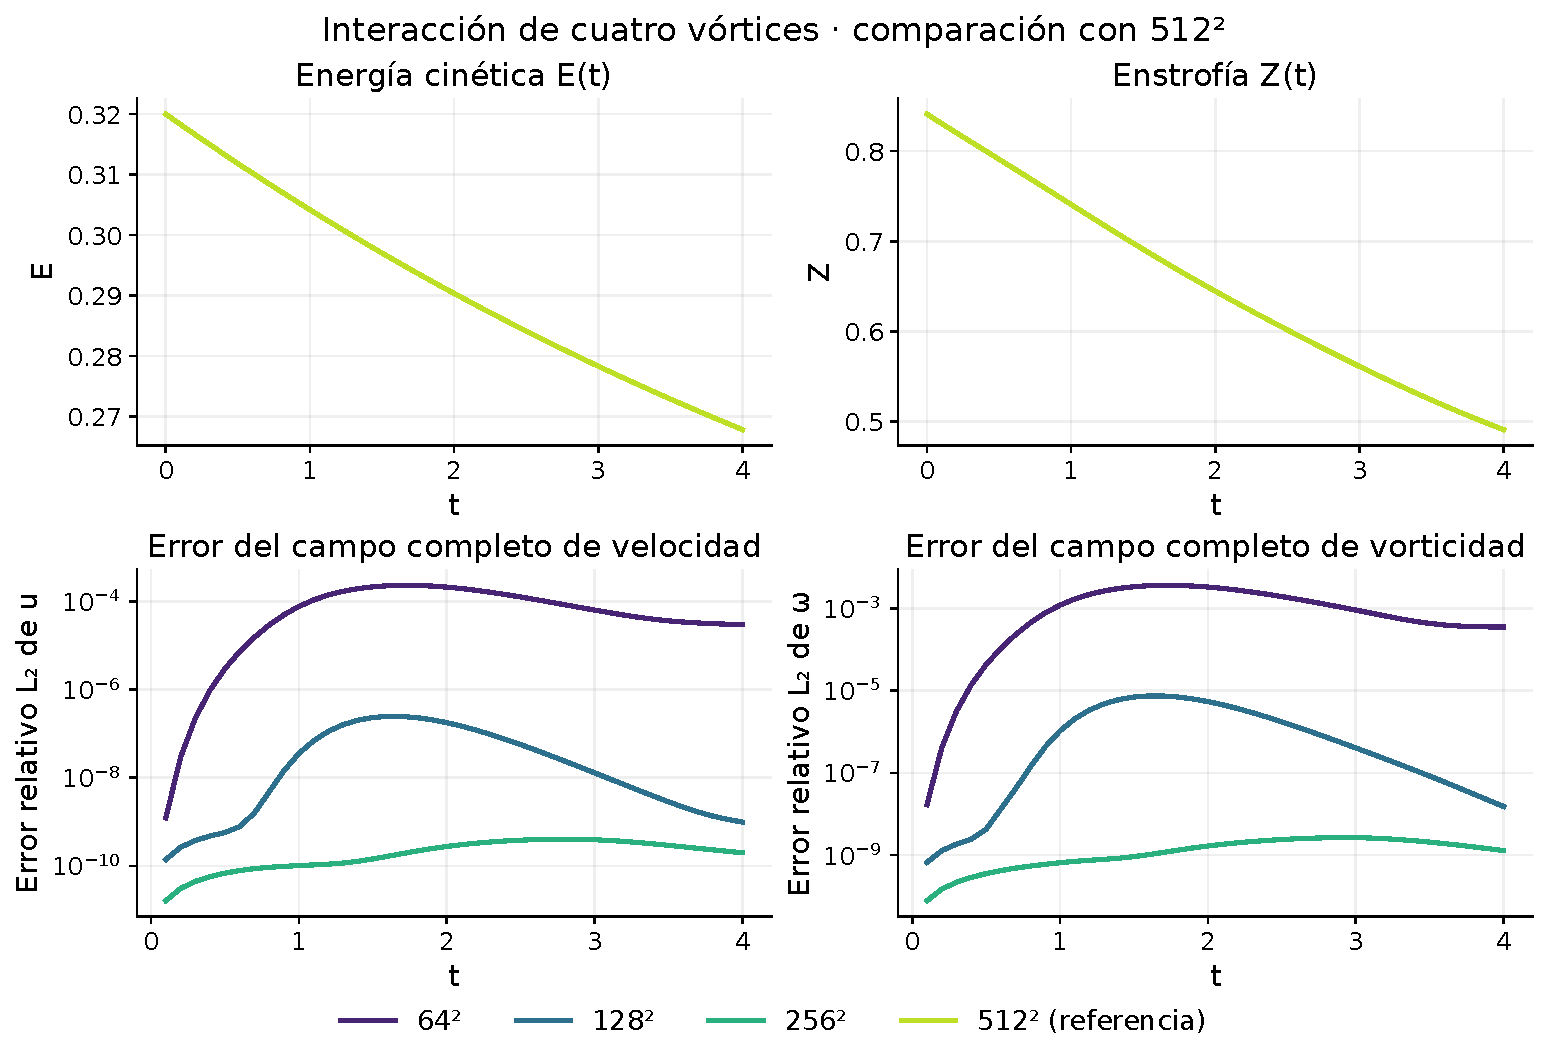
\includegraphics[width=\textwidth,height=.75\textheight,keepaspectratio]{results/research/highres_newtonian_2026-10-14/figures/interacting_vortices_diagnostics_publication.pdf}
\caption{Cuatro vórtices en interacción: energía, enstrofía y errores completos de velocidad y vorticidad durante el intervalo. Las curvas permiten localizar máximos anteriores al tiempo final; la tabla de resolución informa los máximos de toda la secuencia. La versión exploratoria añade espectros y marcadores finales.}
\label{fig:interacting_vortices-diagnostics}\end{figure}
\clearpage
\clearpage
\begin{figure}[p]\centering
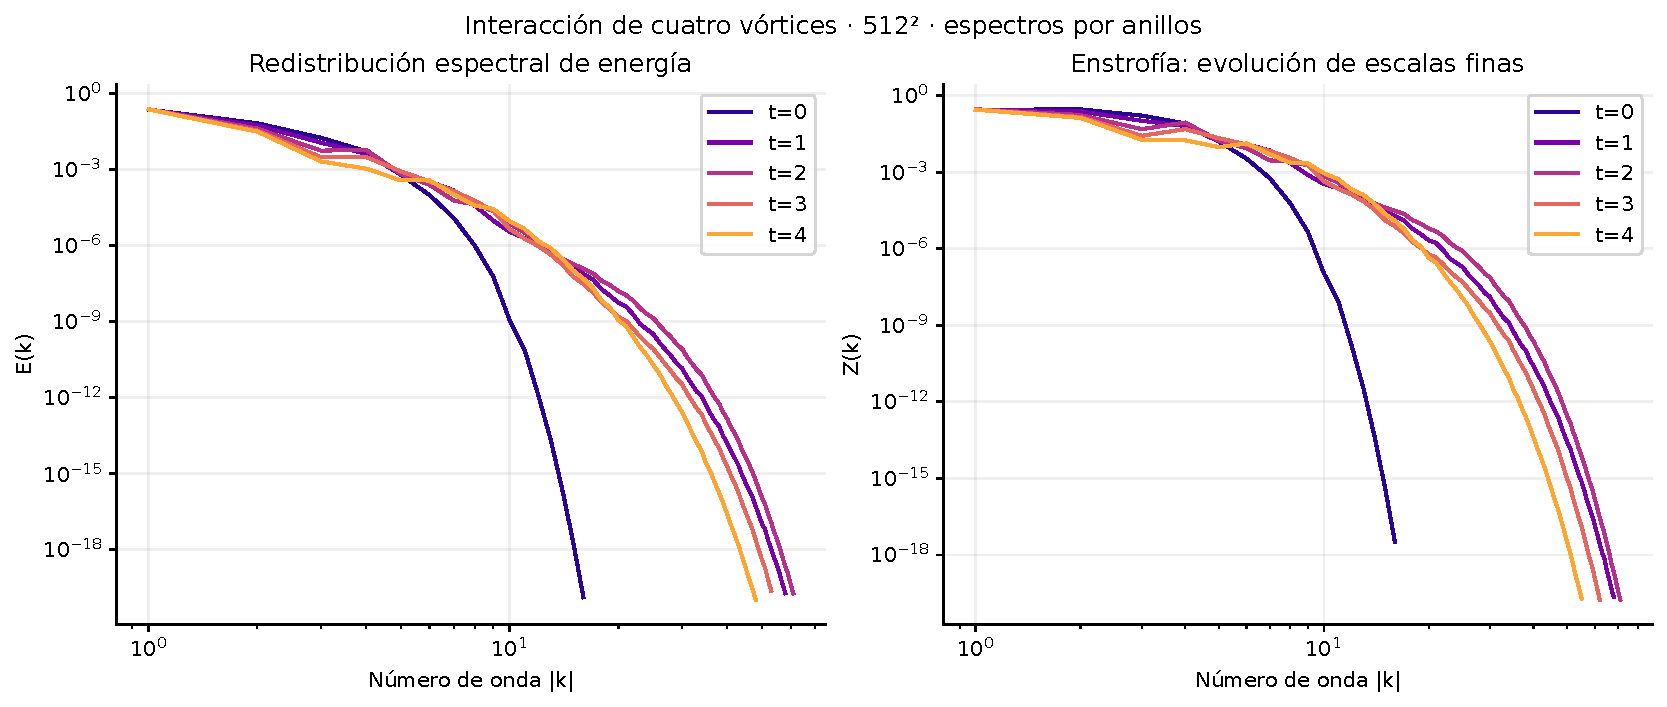
\includegraphics[width=\textwidth,height=.75\textheight,keepaspectratio]{results/research/highres_newtonian_2026-10-14/figures/interacting_vortices_spectra_evolution.pdf}
\caption{Cuatro vórtices en interacción en 512$^2$: evolución de energía y enstrofía por anillos de número de onda. La enstrofía pondera gradientes y complementa la inspección de rapidez. Una cola decreciente aporta evidencia para este flujo e intervalo, sin certificar todas las escalas de otros regímenes.}
\label{fig:interacting_vortices-spectra}\end{figure}
\clearpage
\clearpage
\begin{figure}[p]\centering
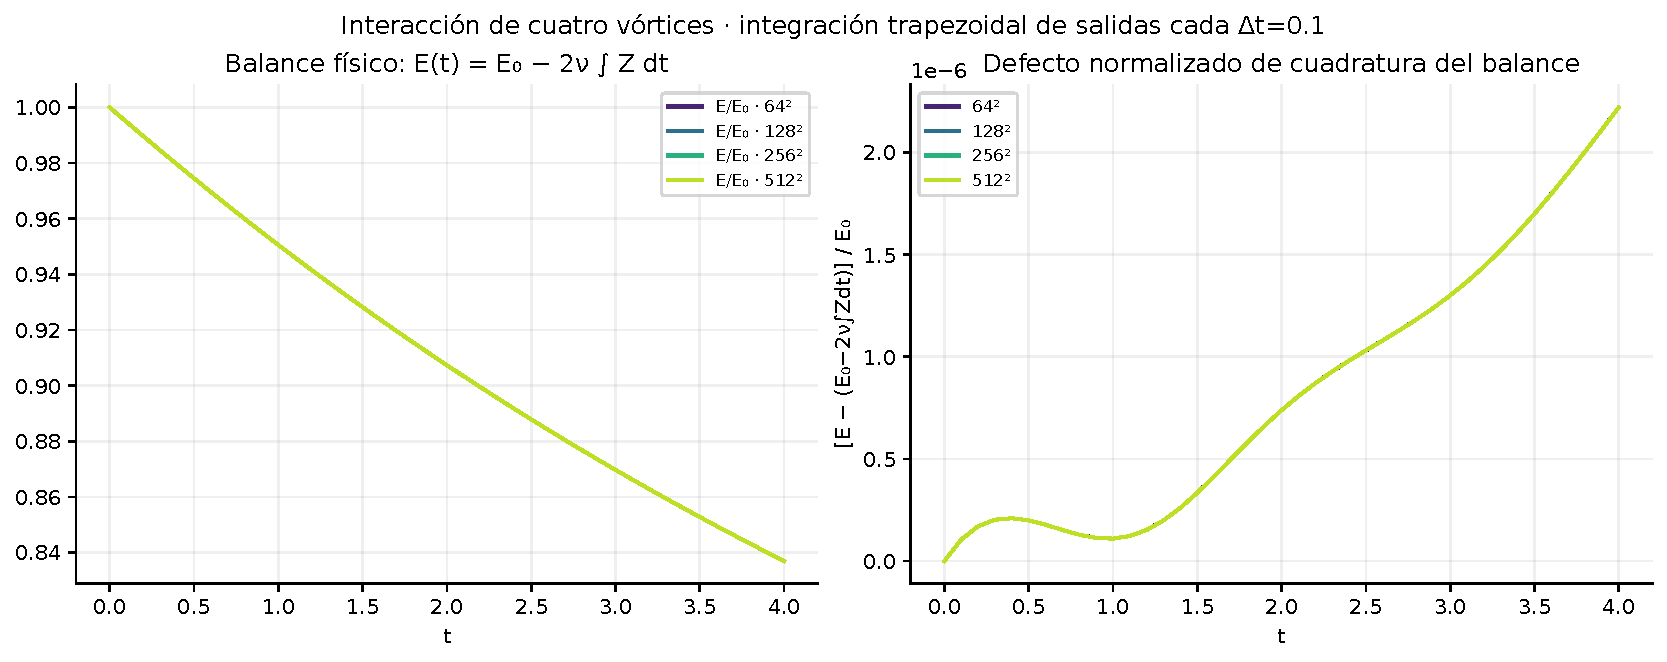
\includegraphics[width=\textwidth,height=.75\textheight,keepaspectratio]{results/research/highres_newtonian_2026-10-14/figures/interacting_vortices_energy_balance.pdf}
\caption{Cuatro vórtices en interacción: energía calculada y energía integrada mediante la disipación viscosa, con defecto normalizado. La integral usa trapecios entre estados guardados; el defecto incluye error de cuadratura temporal de salida y no equivale al error local de los pasos RK4.}
\label{fig:interacting_vortices-energy}\end{figure}
\clearpage
\clearpage
\begin{landscape}
\begin{figure}[p]\centering
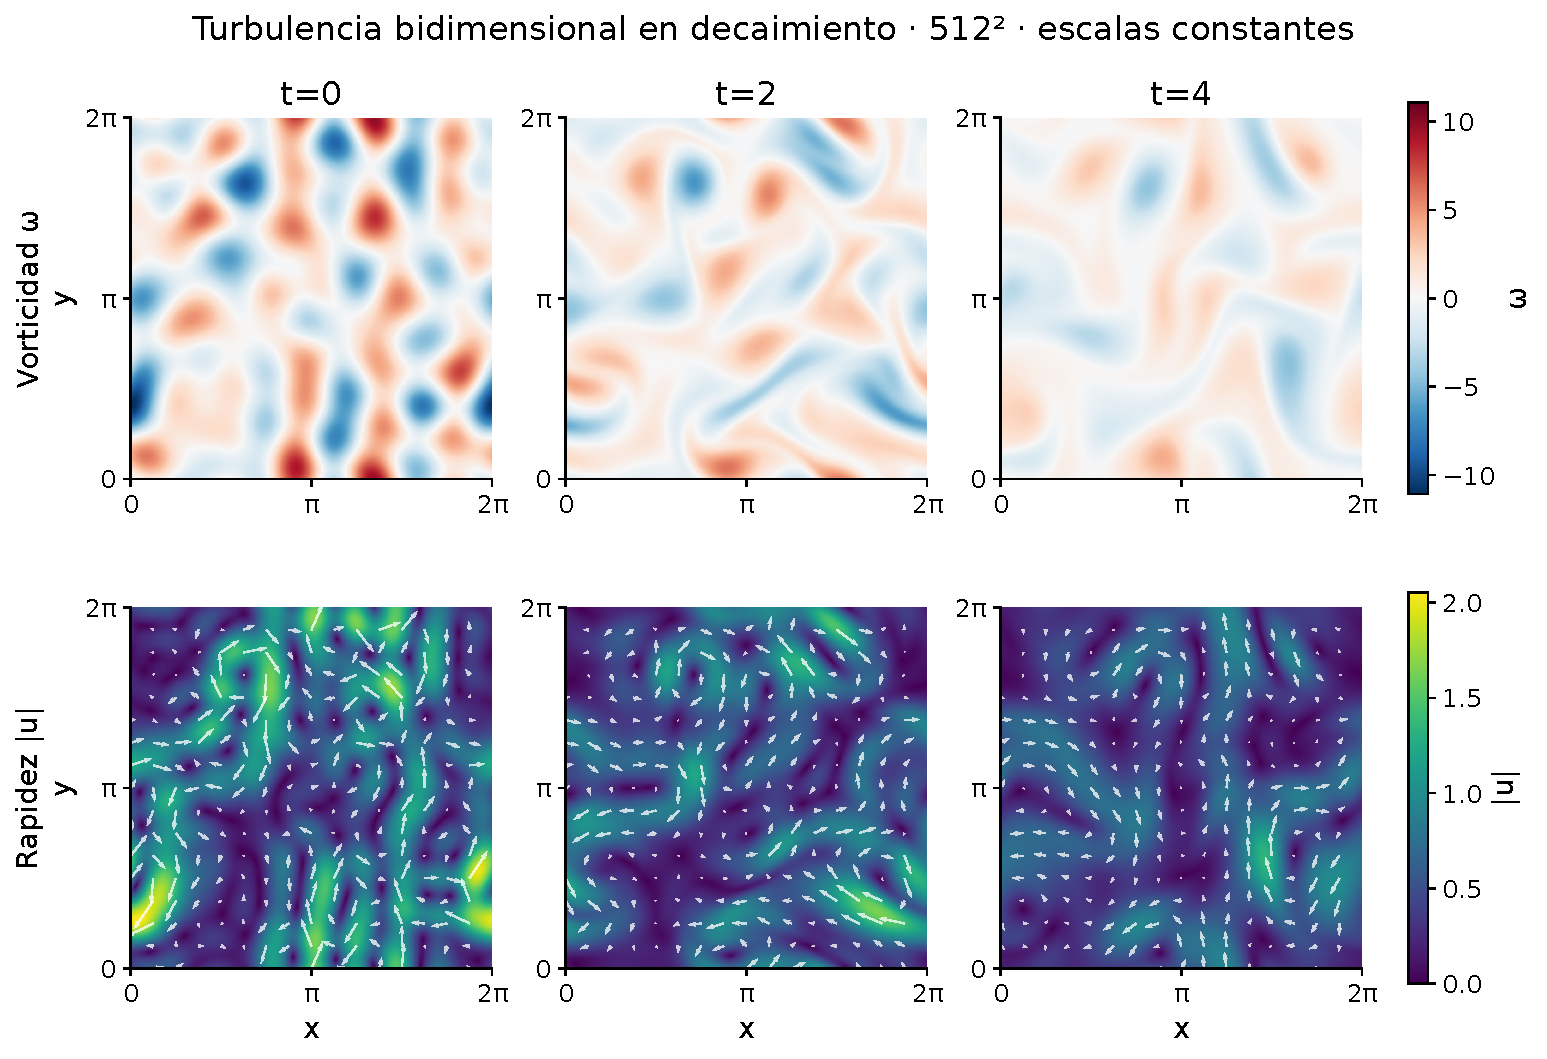
\includegraphics[width=\linewidth,height=.80\textwidth,keepaspectratio]{results/research/highres_newtonian_2026-10-14/figures/decaying_turbulence_evolution_publication.pdf}
\caption{Turbulencia 2D en decaimiento en 512$^2$: tres estados calculados en t=0, t=2 y t=4. Vorticidad con signo y rapidez usan escalas constantes por fila; las flechas muestran velocidad instantánea. Se observan deformación e intercambio de estructura en un dominio periódico, no una estela externa. La secuencia original de cinco tiempos y la animación completa quedan enlazadas como compañeros.}
\label{fig:decaying_turbulence-evolution}\end{figure}
\end{landscape}
\clearpage
\clearpage
\begin{landscape}
\begin{figure}[p]\centering
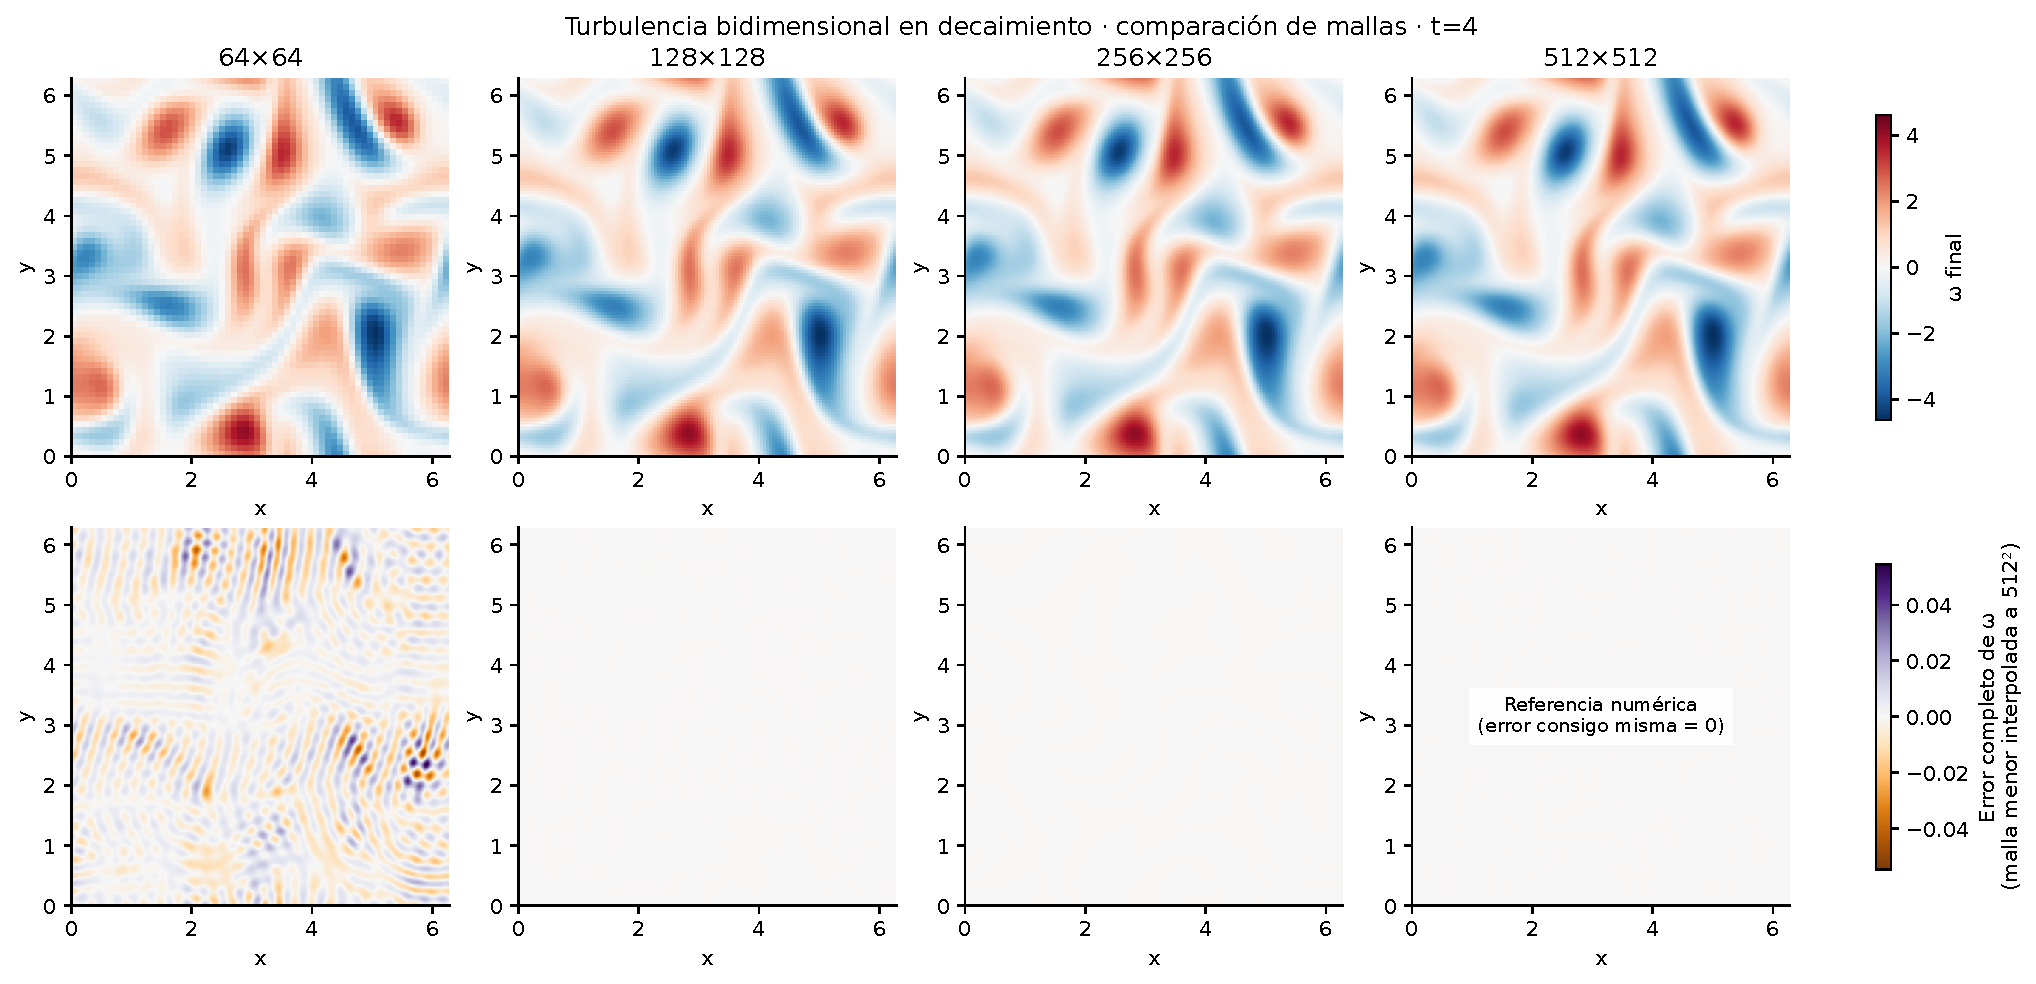
\includegraphics[width=\linewidth,height=.80\textwidth,keepaspectratio]{results/research/highres_newtonian_2026-10-14/figures/decaying_turbulence_grid_comparison.pdf}
\caption{Turbulencia 2D en decaimiento: vorticidad final calculada en cuatro mallas y diferencias de campo completo respecto a 512$^2$. La fila inferior transfiere cada solución gruesa a la malla fina; su barra de error es distinta de la barra física. El panel 512$^2$ se compara consigo mismo y tiene error cero por definición.}
\label{fig:decaying_turbulence-grids}\end{figure}
\end{landscape}
\clearpage
\clearpage
\begin{figure}[p]\centering
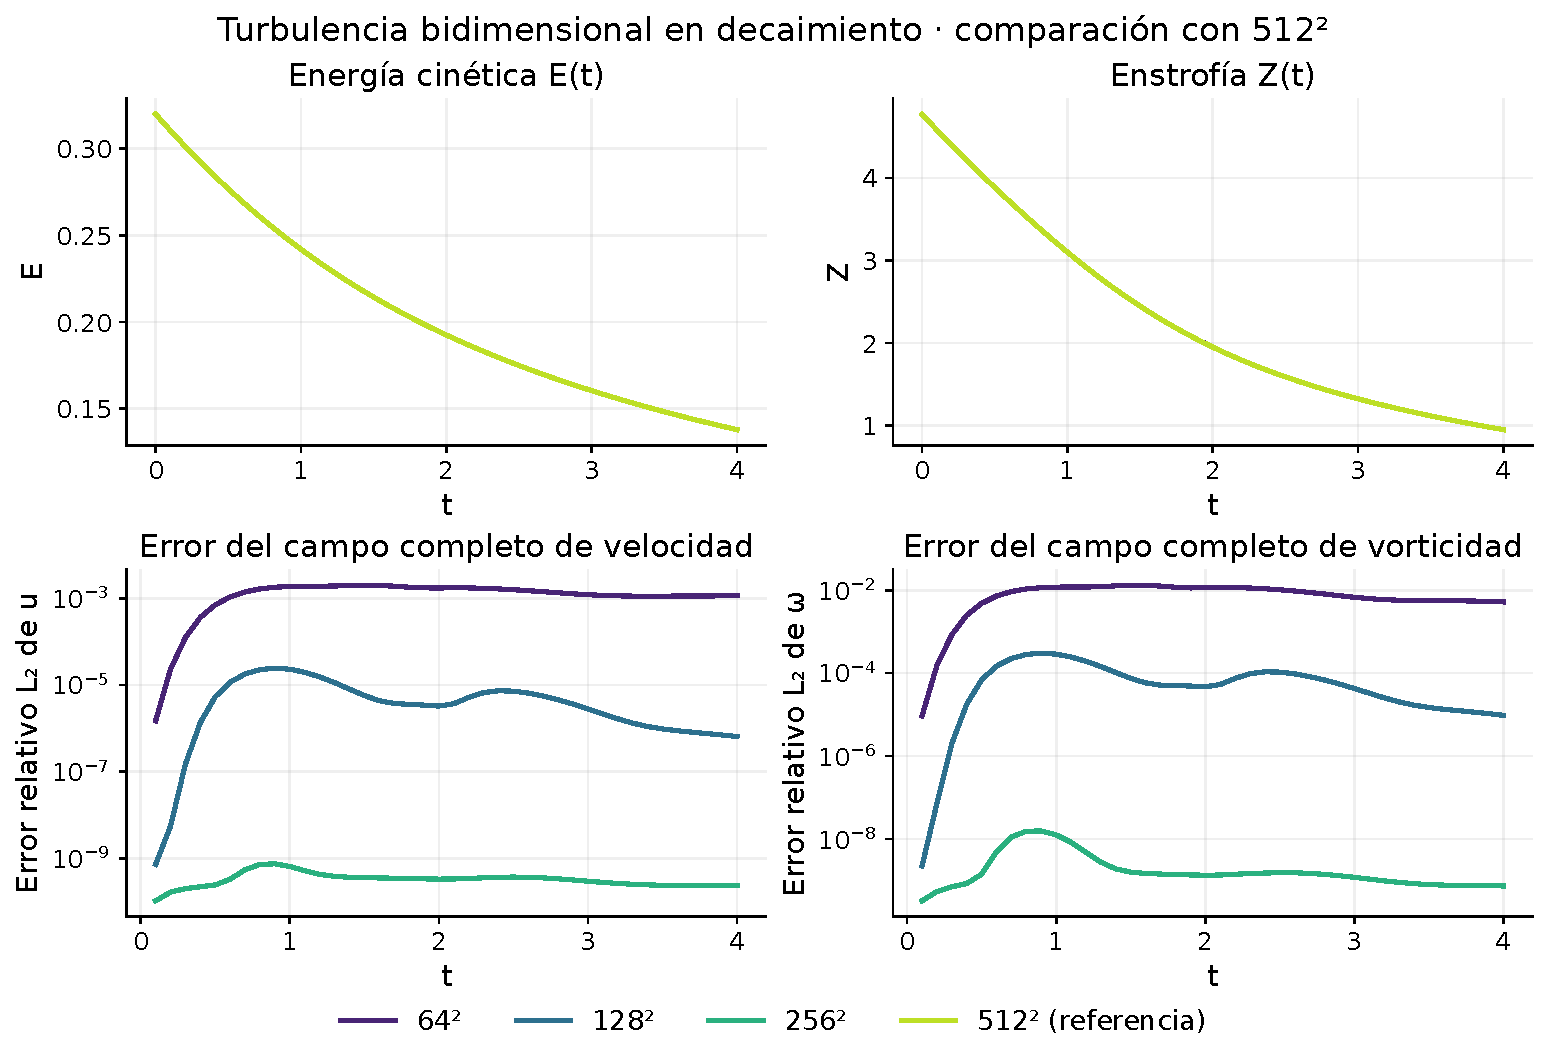
\includegraphics[width=\textwidth,height=.75\textheight,keepaspectratio]{results/research/highres_newtonian_2026-10-14/figures/decaying_turbulence_diagnostics_publication.pdf}
\caption{Turbulencia 2D en decaimiento: energía, enstrofía y errores completos de velocidad y vorticidad durante el intervalo. Las curvas permiten localizar máximos anteriores al tiempo final; la tabla de resolución informa los máximos de toda la secuencia. La versión exploratoria añade espectros y marcadores finales.}
\label{fig:decaying_turbulence-diagnostics}\end{figure}
\clearpage
\clearpage
\begin{figure}[p]\centering
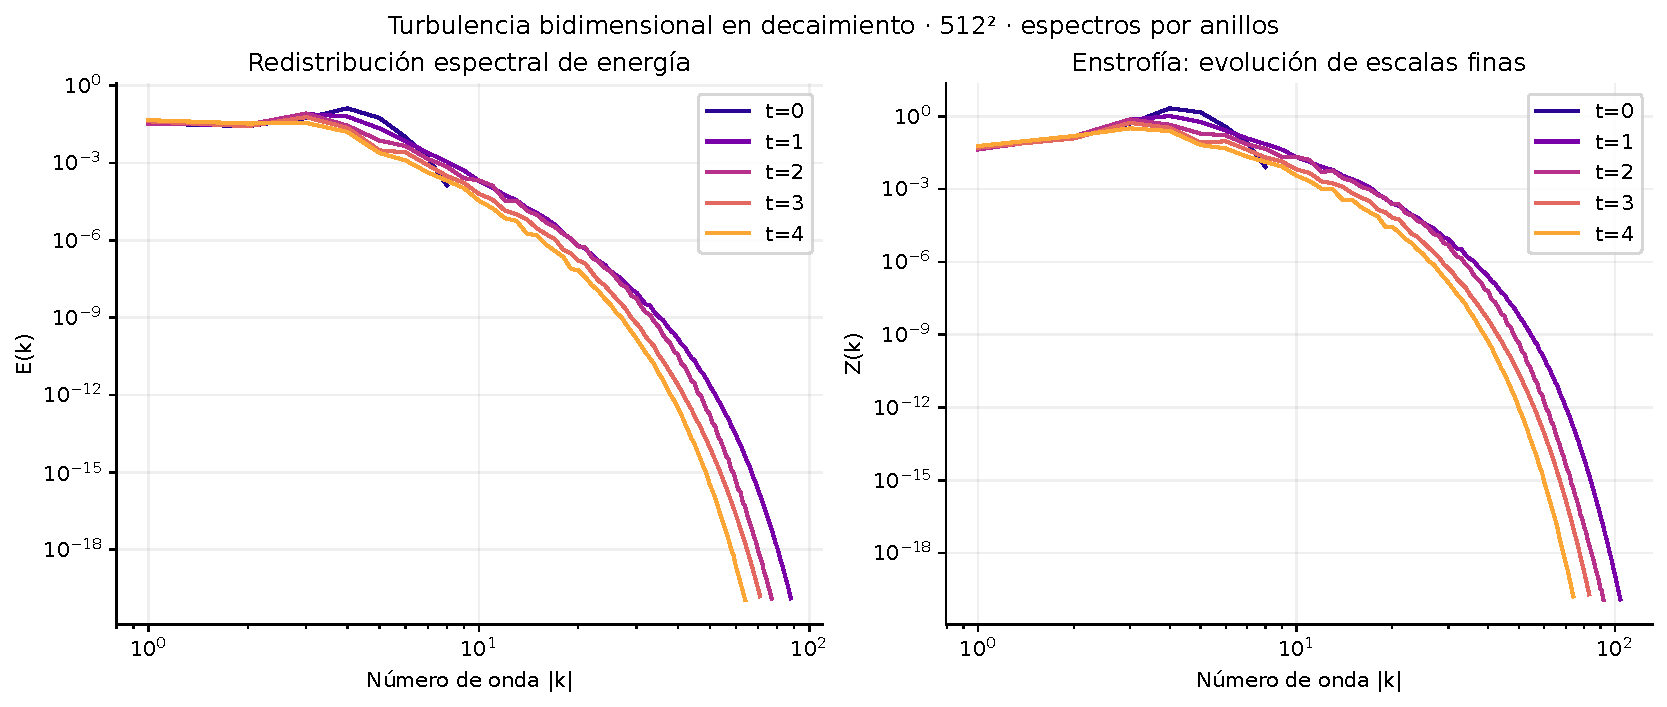
\includegraphics[width=\textwidth,height=.75\textheight,keepaspectratio]{results/research/highres_newtonian_2026-10-14/figures/decaying_turbulence_spectra_evolution.pdf}
\caption{Turbulencia 2D en decaimiento en 512$^2$: evolución de energía y enstrofía por anillos de número de onda. La enstrofía pondera gradientes y complementa la inspección de rapidez. Una cola decreciente aporta evidencia para este flujo e intervalo, sin certificar todas las escalas de otros regímenes.}
\label{fig:decaying_turbulence-spectra}\end{figure}
\clearpage
\clearpage
\begin{figure}[p]\centering
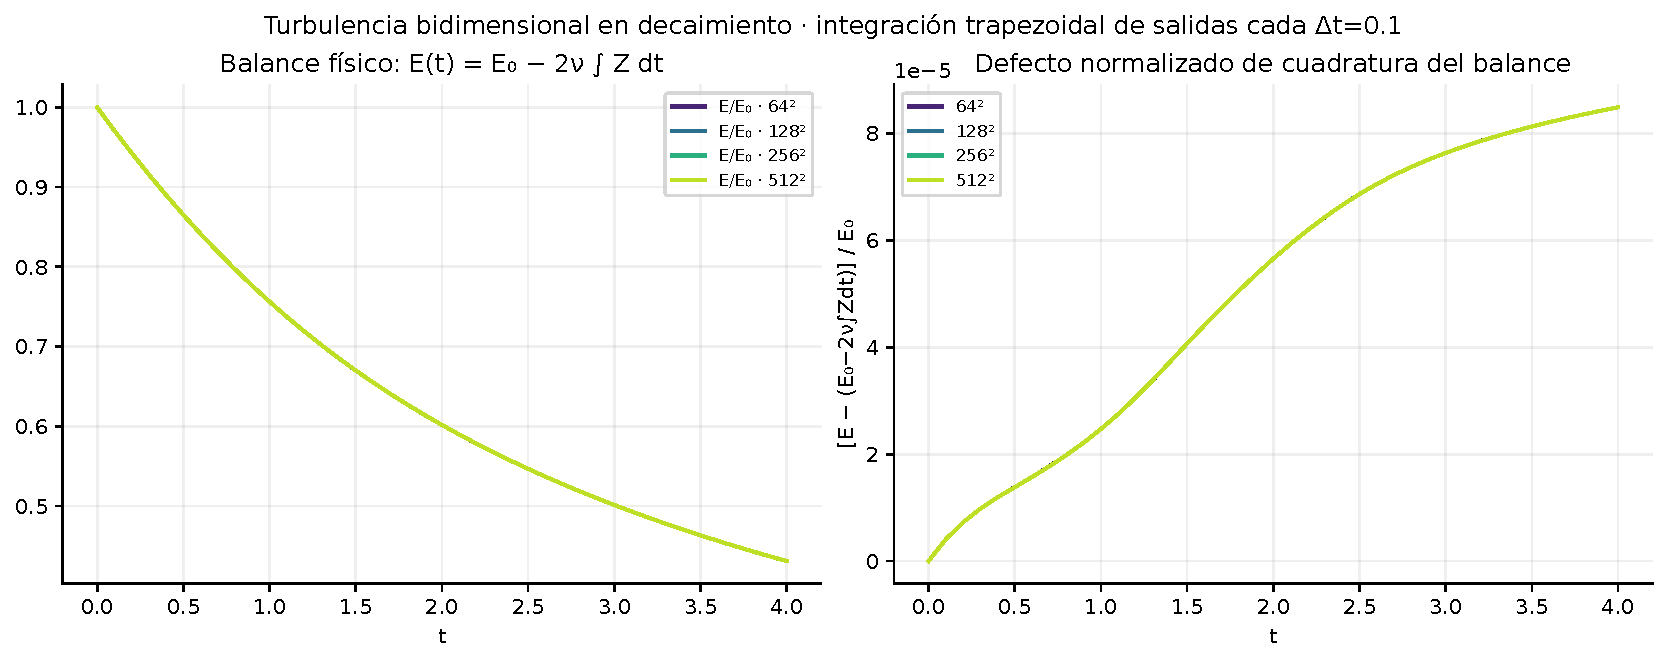
\includegraphics[width=\textwidth,height=.75\textheight,keepaspectratio]{results/research/highres_newtonian_2026-10-14/figures/decaying_turbulence_energy_balance.pdf}
\caption{Turbulencia 2D en decaimiento: energía calculada y energía integrada mediante la disipación viscosa, con defecto normalizado. La integral usa trapecios entre estados guardados; el defecto incluye error de cuadratura temporal de salida y no equivale al error local de los pasos RK4.}
\label{fig:decaying_turbulence-energy}\end{figure}
\clearpage
\begingroup\small\setlength{\tabcolsep}{3pt}
\begin{longtable}{@{}>{\raggedright\arraybackslash}p{4.2cm}>{\raggedright\arraybackslash}p{2.1cm}>{\raggedright\arraybackslash}p{2.4cm}>{\raggedright\arraybackslash}p{3.1cm}>{\raggedright\arraybackslash}p{3.2cm}@{}}
\caption{Control temporal a malla fija, frente a dt nominal 0.00125; máximos en los tiempos guardados.}\\
\toprule
Flujo, 128$^2$ & dt nominal & dt máximo real & Máx. error u & Máx. error $\omega$ \\
\midrule\endfirsthead
\toprule
Flujo, 128$^2$ & dt nominal & dt máximo real & Máx. error u & Máx. error $\omega$ \\
\midrule\endhead
Cuatro vórtices en interacción & 0.005 & 0.005 & 1.955e-07 \% & 1.201e-06 \% \\
Cuatro vórtices en interacción & 0.0025 & 0.0025 & 1.149e-08 \% & 7.054e-08 \% \\
Turbulencia 2D en decaimiento & 0.005 & 0.005 & 1.600e-07 \% & 7.799e-07 \% \\
Turbulencia 2D en decaimiento & 0.0025 & 0.0025 & 9.341e-09 \% & 4.548e-08 \% \\
\bottomrule\end{longtable}\endgroup

Los solvers aplican límites internos de estabilidad, de modo que el paso nominal puede superar el paso real. Se registran ambos y el número de límites activos. El paso mínimo también puede contener ajustes diminutos para alcanzar exactamente un tiempo de salida; no se interpreta por sí solo como rigidez. El orden RK4 se verifica aparte con Taylor–Green analítico en una malla donde los pasos nominales son realmente distintos, mientras que el control Taylor–Green 128$^2$ comprueba la referencia exacta de un único modo y conserva los límites efectivos.

\clearpage
\subsection{\texorpdfstring{Viscoelasticidad: la velocidad puede converger antes que el polímero}{Viscoelasticidad: la velocidad puede converger antes que el polímero}}
Oldroyd-B y FENE-P se integraron con U=0.8, $\nu_s$=0.02, $\nu_p$=0.04, $\lambda$=0.5, y difusión constitutiva $\kappa$=0, hasta T=2.4. FENE-P usa L$^2$=12; Oldroyd-B no tiene un límite de extensibilidad finita. Ambos retienen el tensor C tridimensional en flujo plano. El control newtoniano $\nu$=0.06 tiene la misma velocidad inicial, densidad, dominio, malla fina y tiempos. La diferencia respecto a él representa dinámica constitutiva; no es un error de reconstrucción. El esfuerzo polimérico inicial es cero cuando C=I y no equivale al esfuerzo newtoniano instantáneo.

\begingroup\small\setlength{\tabcolsep}{3pt}
\begin{longtable}{@{}>{\raggedright\arraybackslash}p{2.7318cm}>{\raggedright\arraybackslash}p{1.0732cm}>{\raggedright\arraybackslash}p{1.0732cm}>{\raggedright\arraybackslash}p{2.3416cm}>{\raggedright\arraybackslash}p{2.3416cm}>{\raggedright\arraybackslash}p{2.7318cm}>{\raggedright\arraybackslash}p{2.3416cm}@{}}
\caption{Máximos de campo completo frente a 256$^2$; C$-$I evita ocultar la deformación detrás de la identidad.}\\
\toprule
Modelo & Malla & Ref. & Máx. error u & Máx. error $\omega$ & Máx. error C$-$I & Máx. error $\tau$ \\
\midrule\endfirsthead
\toprule
Modelo & Malla & Ref. & Máx. error u & Máx. error $\omega$ & Máx. error C$-$I & Máx. error $\tau$ \\
\midrule\endhead
Oldroyd-B & 64$^2$ & 256$^2$ & 0.01958 \% & 0.3684 \% & 12.24 \% & 12.24 \% \\
Oldroyd-B & 128$^2$ & 256$^2$ & 8.872e-04 \% & 0.03377 \% & 4.383 \% & 4.383 \% \\
FENE-P & 64$^2$ & 256$^2$ & 0.01214 \% & 0.219 \% & 0.789 \% & 0.8787 \% \\
FENE-P & 128$^2$ & 256$^2$ & 4.738e-04 \% & 0.01715 \% & 0.101 \% & 0.1165 \% \\
\bottomrule\end{longtable}\endgroup

La comparación de C por sí solo puede diluir el error de deformación, porque incluye el tensor identidad. Se evalúa por ello C$-$I además del esfuerzo $\tau$, usando la norma tensorial de todos sus componentes. En t=0 ambos son nulos y su error relativo es indefinido: ese estado se conserva como null y se excluye del máximo relativo, sin asignarle un cero artificial. Las curvas y errores RMS absolutos permanecen en el JSON. La energía fuera de la banda gruesa se registra por separado del error dinámico.

En 128$^2$, Oldroyd-B conserva errores máximos de 4.383 \% en C$-$I y 4.383 \% en esfuerzo frente a 256$^2$, aunque su velocidad sea mucho más precisa. FENE-P presenta 0.101 \% y 0.1165 \% en esas mismas cantidades. Aplicar el nivel exploratorio del 1 \% también al tensor y al esfuerzo deja la memoria de Oldroyd-B por resolver en 128$^2$. La malla 256$^2$ se usa como referencia numérica, sin declararla convergida contra una integración viscoelástica aún más fina.

En la propia referencia Oldroyd-B 256$^2$, la fracción máxima de potencia tensorial en la cola exterior de la banda retenida es 1.157e-04. Supera marginalmente la heurística $10^{-4}$ y refuerza la interpretación condicionada de esa referencia. Una cola pequeña por sí sola no demuestra convergencia; para establecerla se necesita la comparación tensorial contra una ejecución más fina.

\clearpage
\begin{figure}[p]\centering
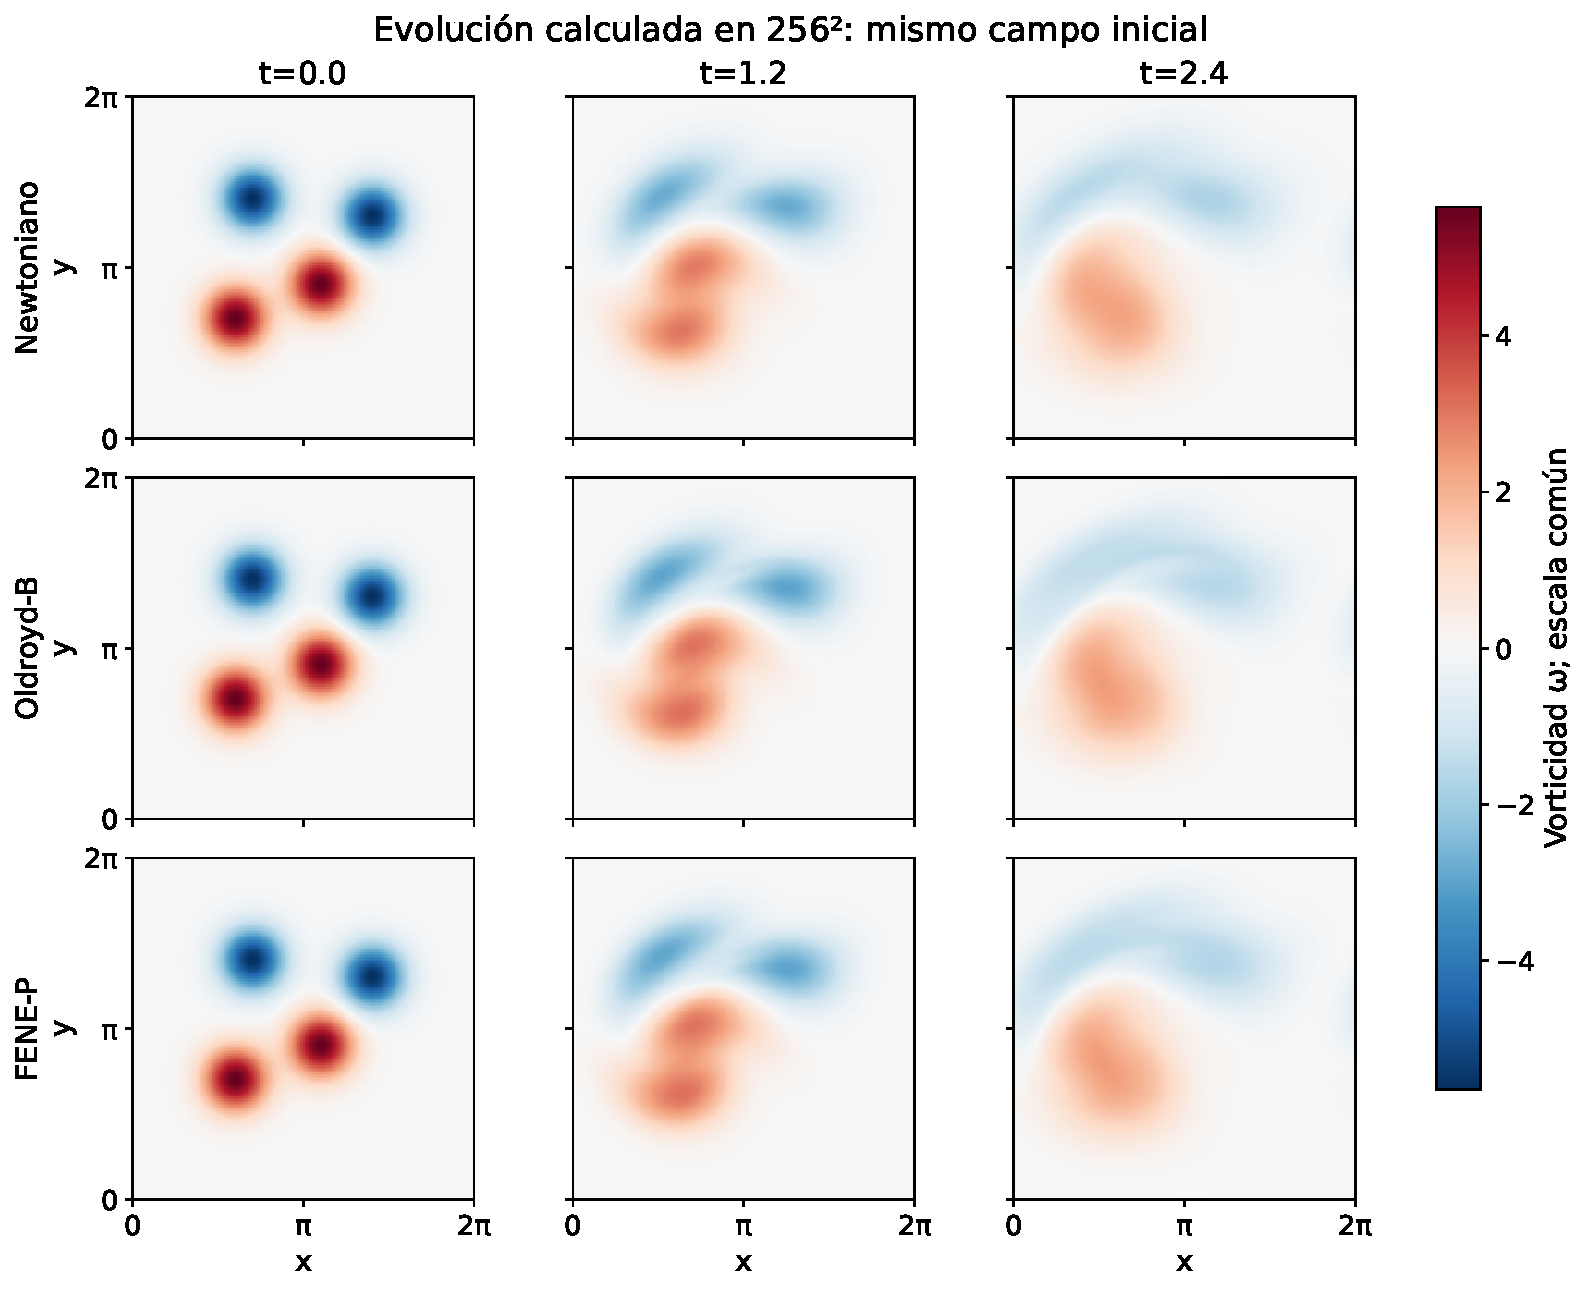
\includegraphics[width=\textwidth,height=.75\textheight,keepaspectratio]{results/research/highres_viscoelastic_2026-10-14/compact_vorticity_evolution.pdf}
\caption{Evolución calculada de vorticidad en 256$^2$ para el control newtoniano, Oldroyd-B y FENE-P, en tres tiempos comunes. La escala con signo se mantiene en los nueve paneles. Las líneas de corriente son instantáneas y los límites del dominio son periódicos.}
\label{fig:ve-vorticity}\end{figure}
\clearpage
\clearpage
\begin{landscape}
\begin{figure}[p]\centering
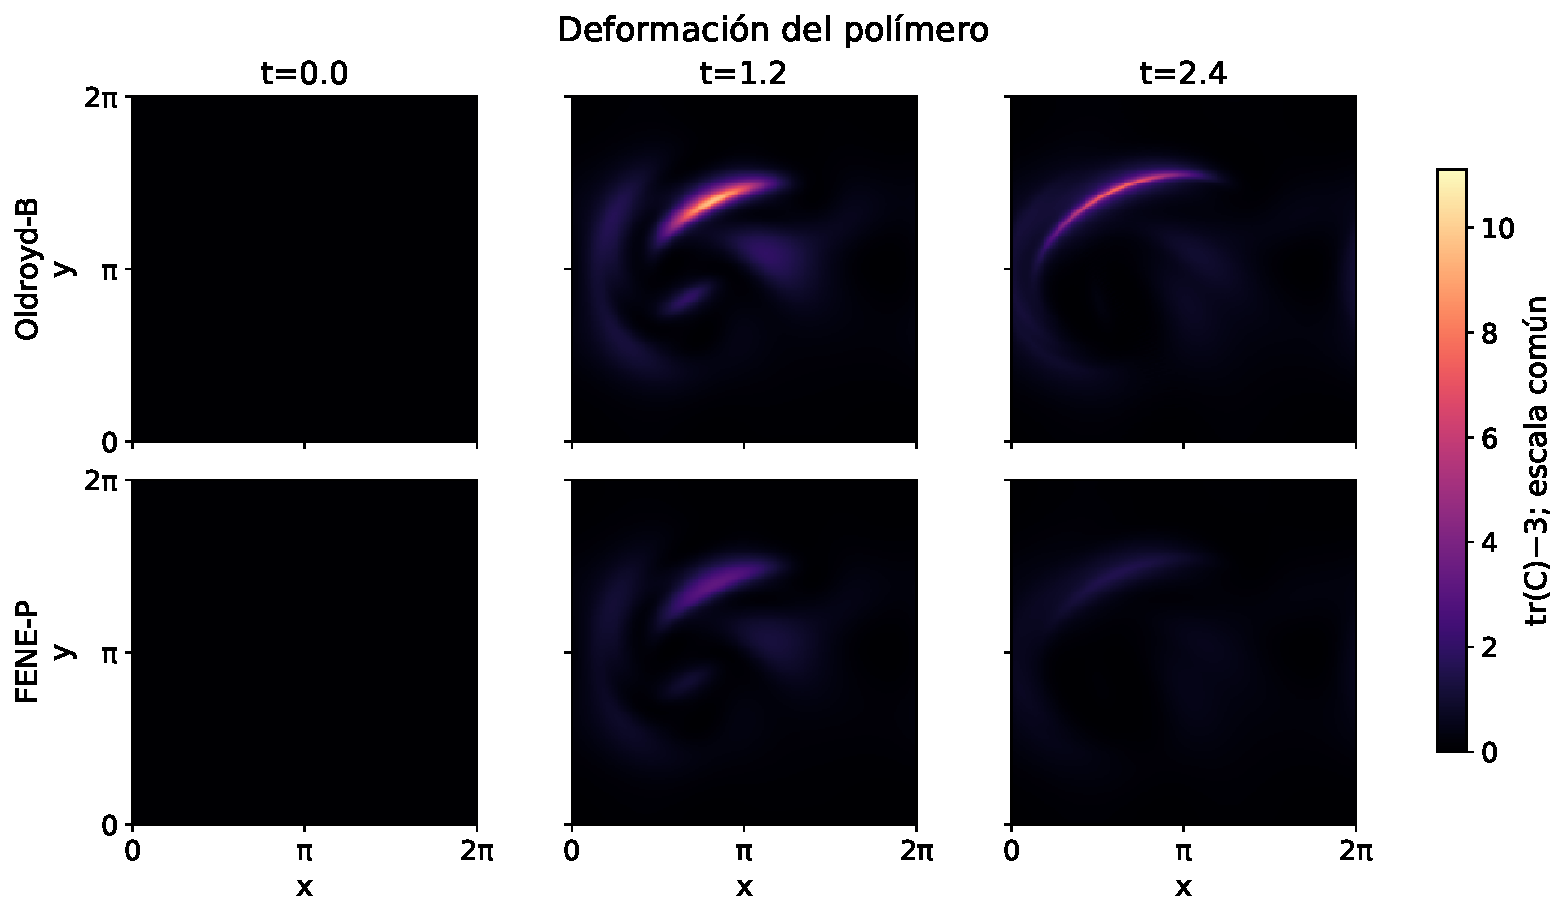
\includegraphics[width=\linewidth,height=.80\textwidth,keepaspectratio]{results/research/highres_viscoelastic_2026-10-14/compact_polymer_trace_evolution.pdf}
\caption{Deformación polimérica tr(C)$-$3 en Oldroyd-B y FENE-P, en 256$^2$ y tres estados calculados. La identidad tridimensional tiene tr(I)=3. El mapa visualiza extensión constitutiva con una escala común por magnitud, sin sustituir la comprobación tensorial completa.}
\label{fig:ve-trace}\end{figure}
\end{landscape}
\clearpage
\clearpage
\begin{landscape}
\begin{figure}[p]\centering
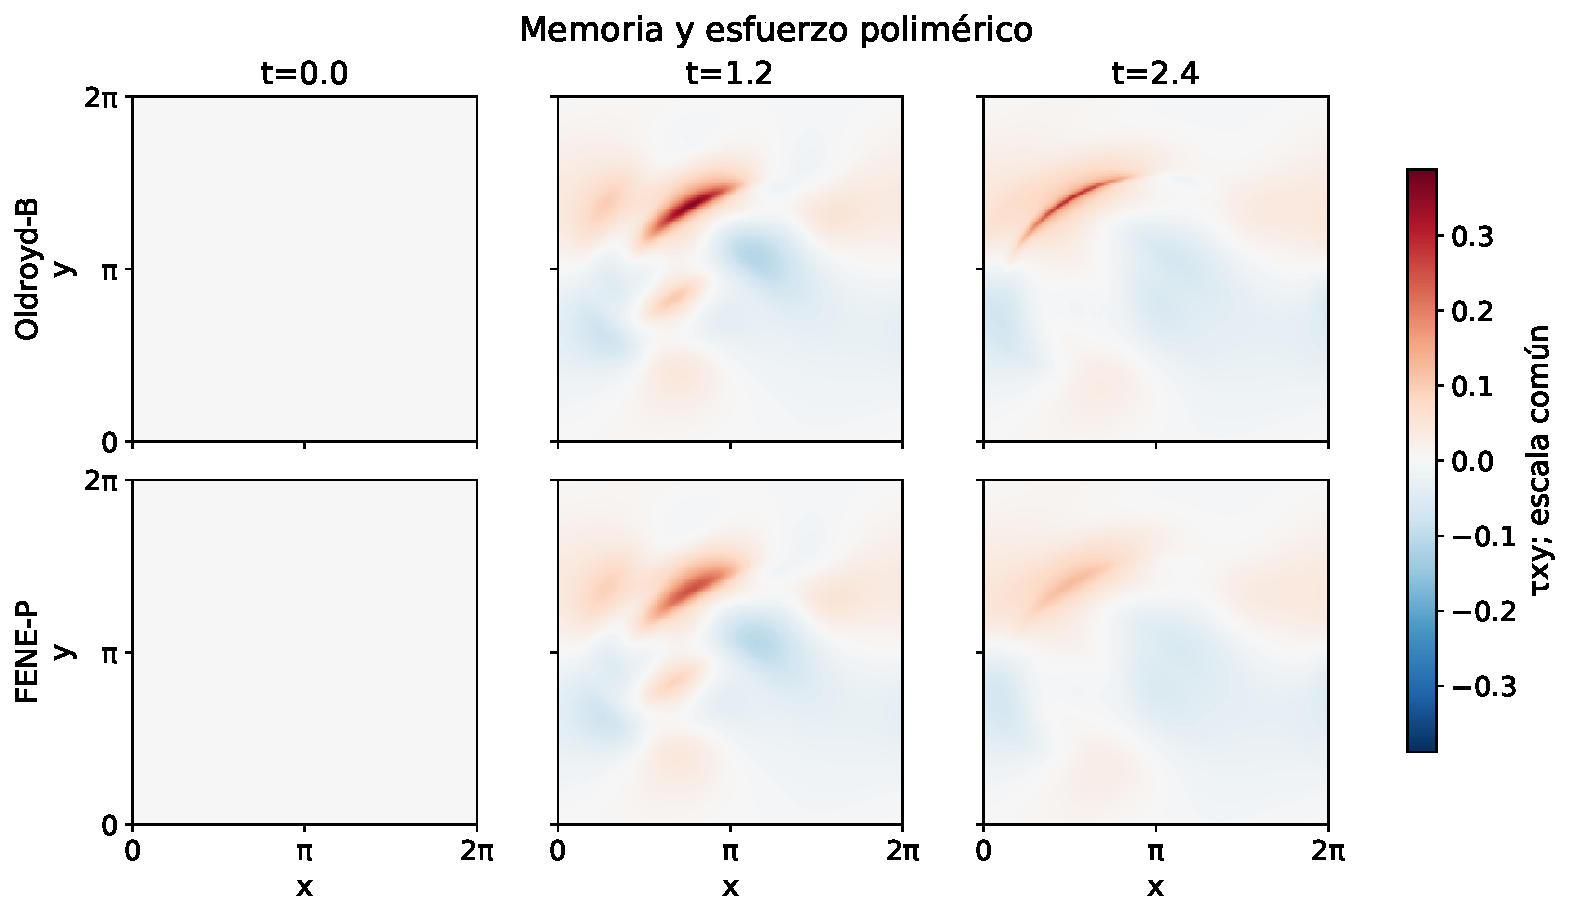
\includegraphics[width=\linewidth,height=.80\textwidth,keepaspectratio]{results/research/highres_viscoelastic_2026-10-14/compact_polymer_stress_evolution.pdf}
\caption{Esfuerzo polimérico cortante $\tau_{xy}$ en Oldroyd-B y FENE-P, en 256$^2$ y tres tiempos comunes. El signo y la barra física se conservan en la secuencia; las bandas de esfuerzo pueden exigir más resolución que un campo de velocidad visualmente suave.}
\label{fig:ve-stress}\end{figure}
\end{landscape}
\clearpage
\clearpage
\begin{figure}[p]\centering
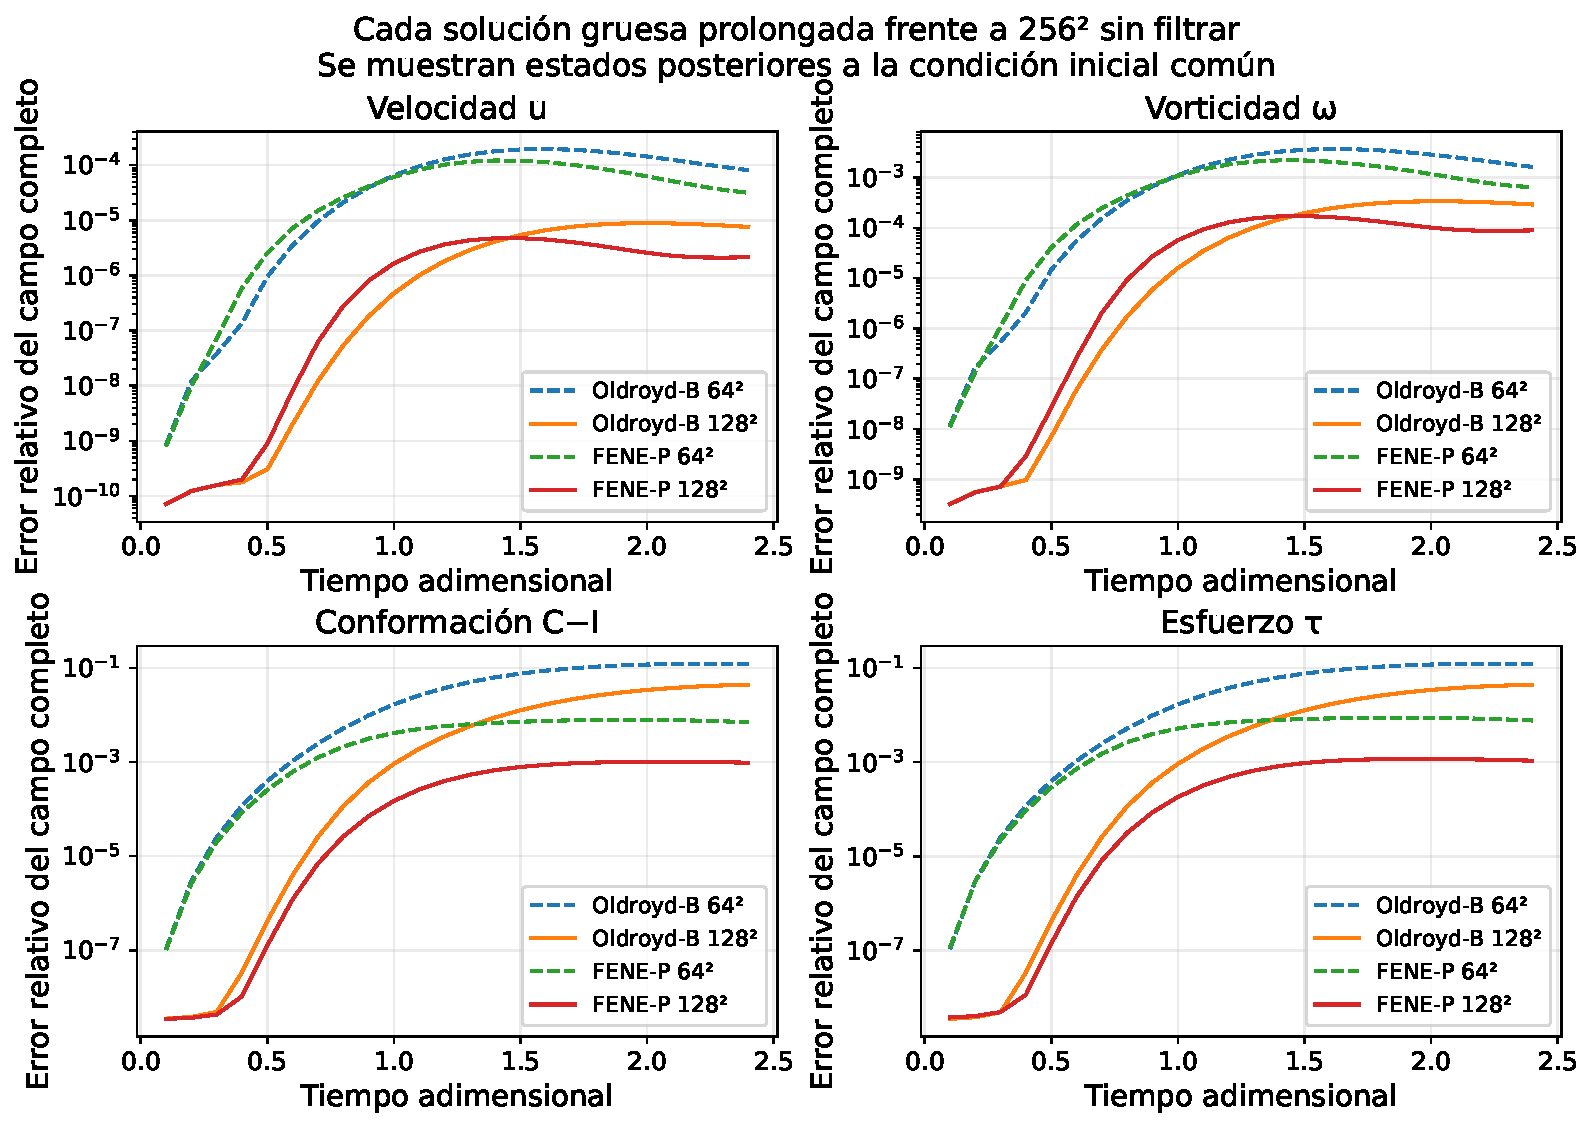
\includegraphics[width=\textwidth,height=.75\textheight,keepaspectratio]{results/research/highres_viscoelastic_2026-10-14/compact_full_field_refinement.pdf}
\caption{Refinamiento viscoelástico frente a 256$^2$: errores completos durante la evolución para velocidad, vorticidad, C$-$I y esfuerzo. Las tablas informan el máximo de estas curvas, incluso cuando éste ocurre antes del estado final. El archivo de análisis también conserva las comparaciones de modos comunes.}
\label{fig:ve-refinement}\end{figure}
\clearpage
\clearpage
\begin{figure}[p]\centering
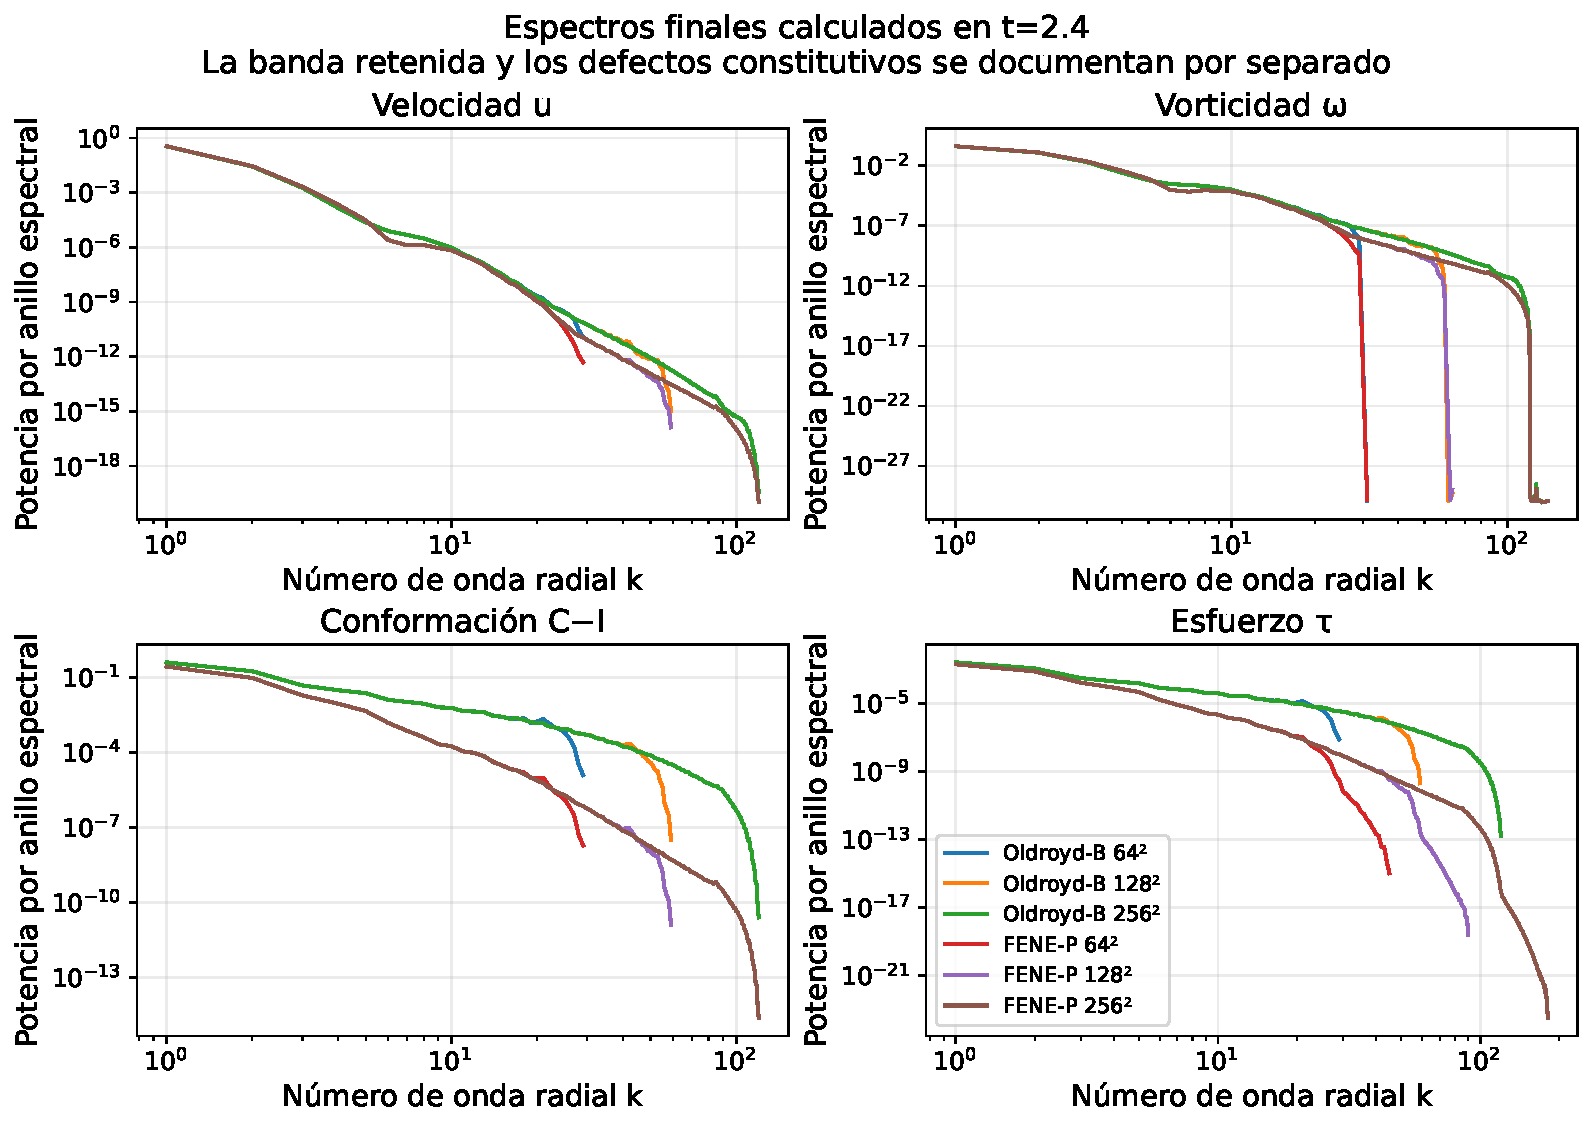
\includegraphics[width=\textwidth,height=.75\textheight,keepaspectratio]{results/research/highres_viscoelastic_2026-10-14/compact_spectral_resolution.pdf}
\caption{Espectros viscoelásticos finales de velocidad, deformación y esfuerzo. Los campos constitutivos derivados, especialmente FENE-P, pueden generar frecuencias adicionales aunque C se integre en una banda de Fourier truncada. La inspección del espectro complementa las comparaciones de campo completo.}
\label{fig:ve-spectra}\end{figure}
\clearpage
\clearpage
\begin{figure}[p]\centering
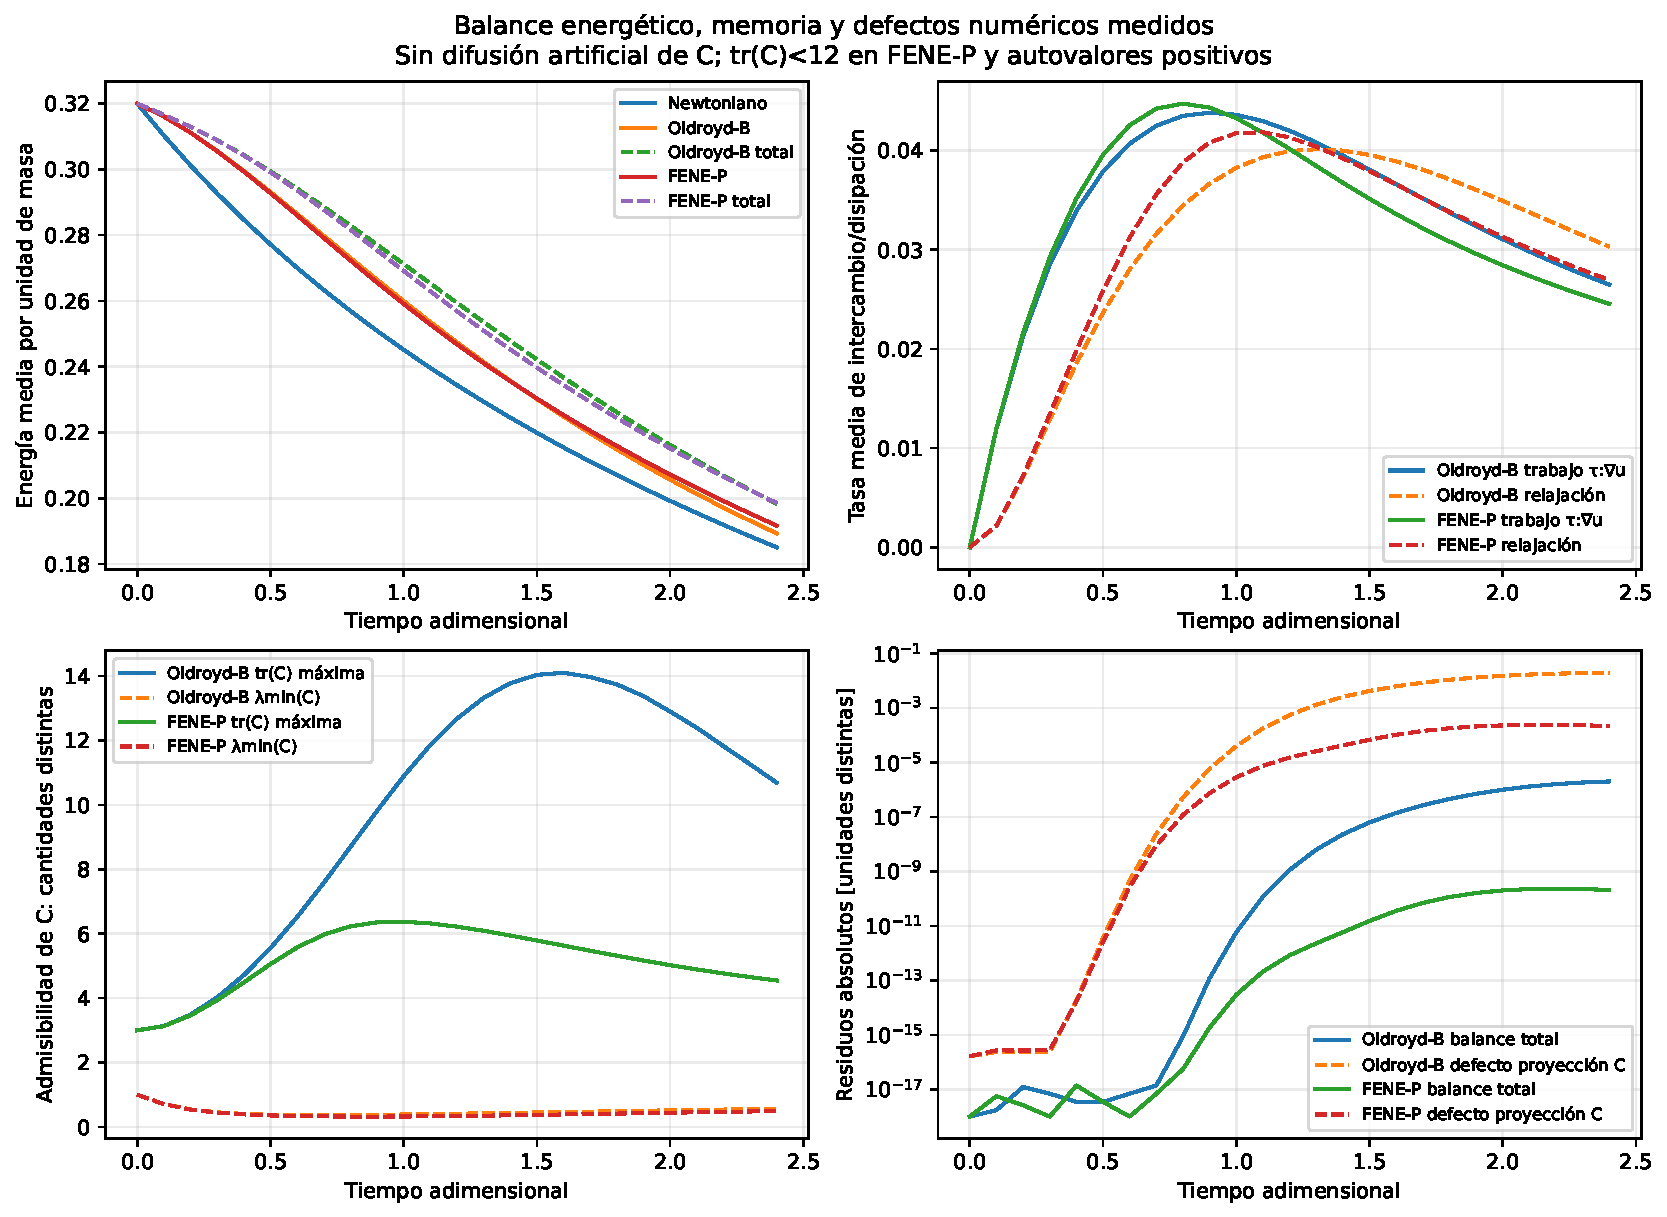
\includegraphics[width=\textwidth,height=.75\textheight,keepaspectratio]{results/research/highres_viscoelastic_2026-10-14/energy_memory_and_residuals.pdf}
\caption{Intercambio de energía cinética y energía libre del polímero, memoria constitutiva y residuos medidos. Se distinguen el balance del operador semidiscreto, el defecto espacial de proyección y el residuo temporal calculado desde snapshots. Este último incorpora el error de diferenciación entre salidas.}
\label{fig:ve-energy}\end{figure}
\clearpage
\begingroup\small\setlength{\tabcolsep}{3pt}
\begin{longtable}{@{}>{\raggedright\arraybackslash}p{2.8cm}>{\raggedright\arraybackslash}p{2.6cm}>{\raggedright\arraybackslash}p{2.8cm}>{\raggedright\arraybackslash}p{2.8cm}>{\raggedright\arraybackslash}p{4.0cm}@{}}
\caption{Admisibilidad en etapas internas de la malla fina y balance semidiscreto relativo; no son errores contra limpio.}\\
\toprule
Modelo & Wi de referencia & Mín. autovalor C & Máx. tr(C) & Defecto / pico disipación \\
\midrule\endfirsthead
\toprule
Modelo & Wi de referencia & Mín. autovalor C & Máx. tr(C) & Defecto / pico disipación \\
\midrule\endhead
Oldroyd-B & 0.9794 & 0.3648 & 14.11 & 0.003405 \% \\
FENE-P & 0.9794 & 0.3205 & 6.376 & 3.734e-07 \% \\
\bottomrule\end{longtable}\endgroup

\begingroup\small\setlength{\tabcolsep}{3pt}
\begin{longtable}{@{}>{\raggedright\arraybackslash}p{3.0cm}>{\raggedright\arraybackslash}p{3.0cm}>{\raggedright\arraybackslash}p{3.0cm}>{\raggedright\arraybackslash}p{3.0cm}>{\raggedright\arraybackslash}p{3.0cm}@{}}
\caption{Control temporal separado en 128$^2$: dt nominal 0.004 frente a 0.002, con límites efectivos explícitos.}\\
\toprule
Modelo, 128$^2$ & dt máximo real & dt máximo real ref. & Máx. error u & Máx. error $\tau$ \\
\midrule\endfirsthead
\toprule
Modelo, 128$^2$ & dt máximo real & dt máximo real ref. & Máx. error u & Máx. error $\tau$ \\
\midrule\endhead
Oldroyd-B & 0.004 & 0.002 & 3.130e-08 \% & 1.514e-05 \% \\
FENE-P & 0.004 & 0.002 & 1.937e-08 \% & 1.935e-06 \% \\
\bottomrule\end{longtable}\endgroup

La positividad de C y el límite de traza de FENE-P se comprueban en etapas internas; los pasos que los violan se rechazan y se registra su reducción, sin recortar el tensor. Los residuos constitutivos y energéticos son medidos y pueden ser no nulos. El control dt/2 acota el efecto temporal en 128$^2$; no sustituye el refinamiento espacial ni extiende la conclusión a alto Weissenberg, paredes, cilindros o tridimensionalidad.

\clearpage
\subsection{\texorpdfstring{Viscoplasticidad: corte, viscosidad y esfuerzo con horizontes separados}{Viscoplasticidad: corte, viscosidad y esfuerzo con horizontes separados}}
Herschel--Bulkley adelgazante ($n=0.6$), Bingham ($n=1$) y Herschel--Bulkley espesante ($n=1.4$) parten de la misma velocidad de cuatro vórtices, $U=0.8$. El esfuerzo de cedencia es $\tau_y=0.01$, $m=10$ y $\epsilon=0.001$. La consistencia $K$ se ajusta para que la viscosidad aparente sea 0.04 a la tasa declarada $\dot\gamma=1.959$. Igualar un punto de las curvas no hace equivalentes los materiales en todas las tasas ni iguala automáticamente sus Reynolds. Los modelos son regularizados e inelásticos; sus zonas de bajo esfuerzo siguen admitiendo deformación.

\begingroup\small\setlength{\tabcolsep}{3pt}
\begin{longtable}{@{}>{\raggedright\arraybackslash}p{2.9691cm}>{\raggedright\arraybackslash}p{1.3856cm}>{\raggedright\arraybackslash}p{2.5732cm}>{\raggedright\arraybackslash}p{2.5732cm}>{\raggedright\arraybackslash}p{2.6722cm}>{\raggedright\arraybackslash}p{2.6722cm}@{}}
\caption{Evolución larga, 0$\leq$t$\leq$2: 64$^2$ frente a 128$^2$; máximos completos y norma física del esfuerzo.}\\
\toprule
Material & Malla & Máx. error u & Máx. error $\omega$ & Máx. error $\tau$ & Máx. error $\eta$ \\
\midrule\endfirsthead
\toprule
Material & Malla & Máx. error u & Máx. error $\omega$ & Máx. error $\tau$ & Máx. error $\eta$ \\
\midrule\endhead
Bingham regularizado & 64$^2$ & 0.01547 \% & 0.2662 \% & 0.496 \% & 2.399 \% \\
HB espesante & 64$^2$ & 0.01671 \% & 0.3024 \% & 0.4498 \% & 2.452 \% \\
HB adelgazante & 64$^2$ & 0.0227 \% & 0.3775 \% & 0.963 \% & 7.906 \% \\
\bottomrule\end{longtable}\endgroup

\begingroup\small\setlength{\tabcolsep}{3pt}
\begin{longtable}{@{}>{\raggedright\arraybackslash}p{2.9691cm}>{\raggedright\arraybackslash}p{1.3856cm}>{\raggedright\arraybackslash}p{2.5732cm}>{\raggedright\arraybackslash}p{2.5732cm}>{\raggedright\arraybackslash}p{2.6722cm}>{\raggedright\arraybackslash}p{2.6722cm}@{}}
\caption{Referencia corta, 0$\leq$t$\leq$0.1: comparación frente a 256$^2$; máximos completos y norma física del esfuerzo.}\\
\toprule
Material & Malla & Máx. error u & Máx. error $\omega$ & Máx. error $\tau$ & Máx. error $\eta$ \\
\midrule\endfirsthead
\toprule
Material & Malla & Máx. error u & Máx. error $\omega$ & Máx. error $\tau$ & Máx. error $\eta$ \\
\midrule\endhead
Bingham regularizado & 64$^2$ & 0.01462 \% & 0.2579 \% & 0.4848 \% & 2.382 \% \\
Bingham regularizado & 128$^2$ & 0.001559 \% & 0.0497 \% & 0.1157 \% & 0.8218 \% \\
HB espesante & 64$^2$ & 0.01427 \% & 0.2655 \% & 0.4043 \% & 2.513 \% \\
HB espesante & 128$^2$ & 0.002165 \% & 0.0684 \% & 0.114 \% & 0.8806 \% \\
HB adelgazante & 64$^2$ & 0.02261 \% & 0.3776 \% & 0.946 \% & 7.095 \% \\
HB adelgazante & 128$^2$ & 0.001963 \% & 0.06539 \% & 0.2714 \% & 5.023 \% \\
\bottomrule\end{longtable}\endgroup

La referencia $256^2$ sólo cubre $t\leq0.1$ y contiene dos salidas, $t=0$ y $t=0.1$. Su concordancia no valida el horizonte completo hasta $t=2$. La evolución larga tiene únicamente el control $64^2/128^2$ y conserva errores de velocidad, vorticidad, corte, viscosidad y esfuerzo. El esfuerzo simétrico se evalúa con Frobenius, $\tau_{xx}^2+2\tau_{xy}^2+\tau_{yy}^2$; el comparador primario conserva también la norma del vector empaquetado de tres componentes, que no es idéntica.

La viscosidad aparente HB adelgazante conserva un máximo de diferencia completa 7.906 \% en la comparación larga 64$^2$/128$^2$, y de 5.023 \% en 128$^2$ frente a 256$^2$ durante el horizonte corto. Los errores pequeños de velocidad y esfuerzo no bastan para declarar convergido ese campo constitutivo. La ley regularizada es especialmente sensible a diferencias de corte cerca de tasas pequeñas.

\clearpage
\begin{figure}[p]\centering
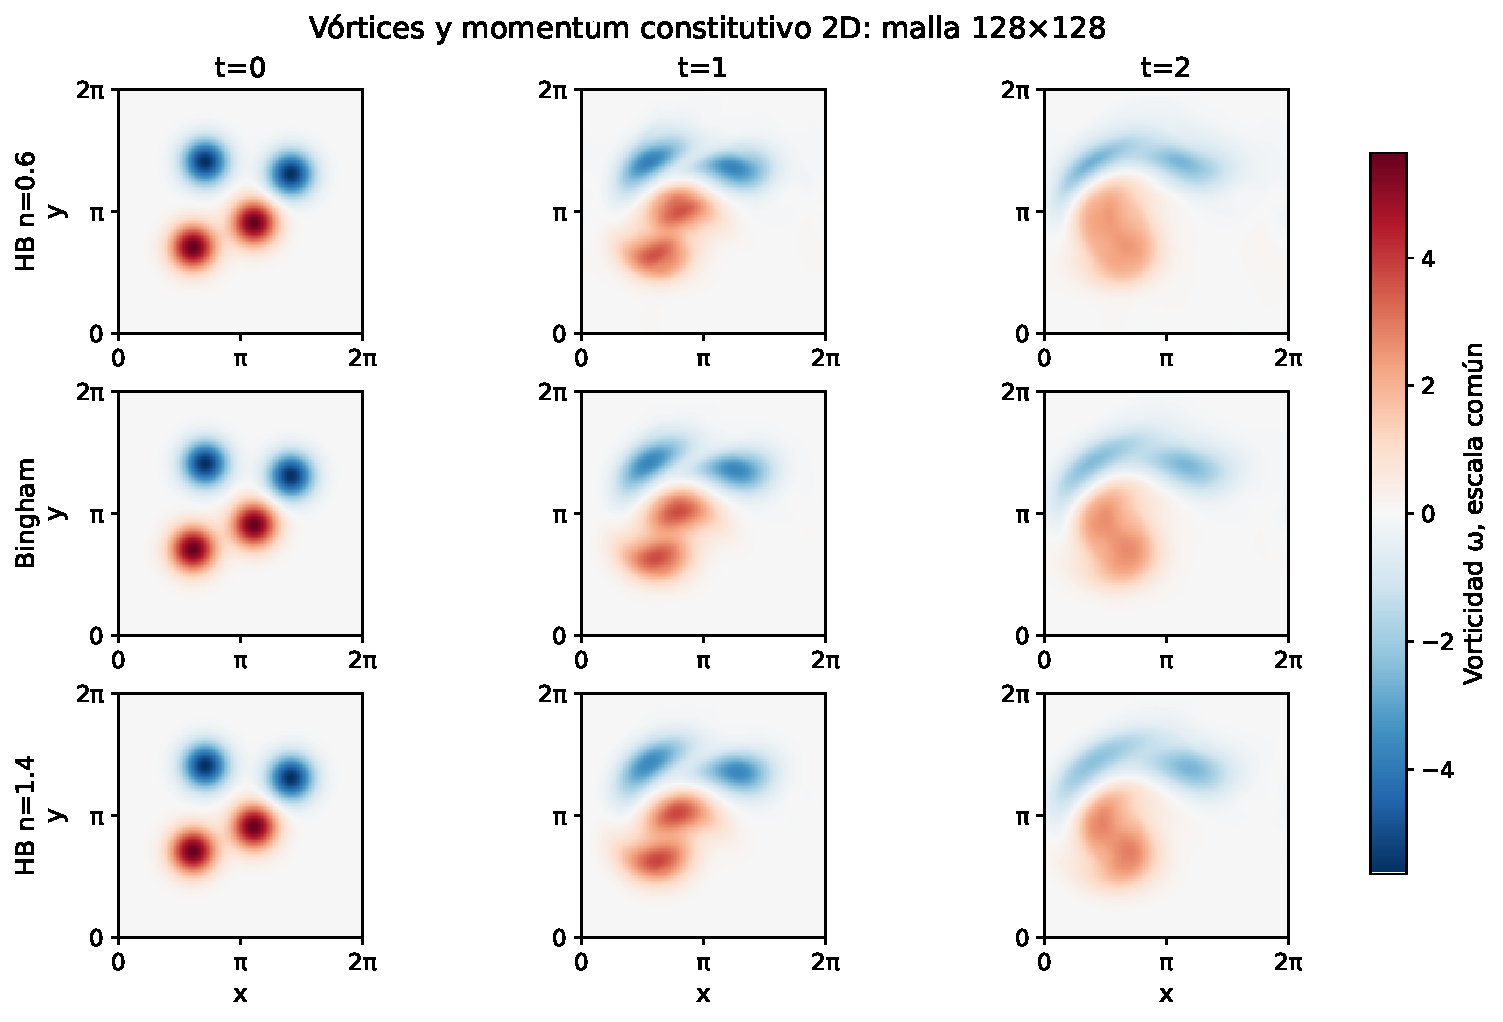
\includegraphics[width=\textwidth,height=.75\textheight,keepaspectratio]{results/research/highres_viscoplastic_2026-10-14/figures/vorticity_publication.pdf}
\caption{Evolución real de los tres materiales viscoplásticos en 128$^2$: tres tiempos del horizonte hasta t=2. La escala de vorticidad es común para todos los paneles y revela deformación, desplazamiento y difusión bajo condiciones iniciales iguales.}
\label{fig:vp-vorticity}\end{figure}
\clearpage
\clearpage
\begin{landscape}
\begin{figure}[p]\centering
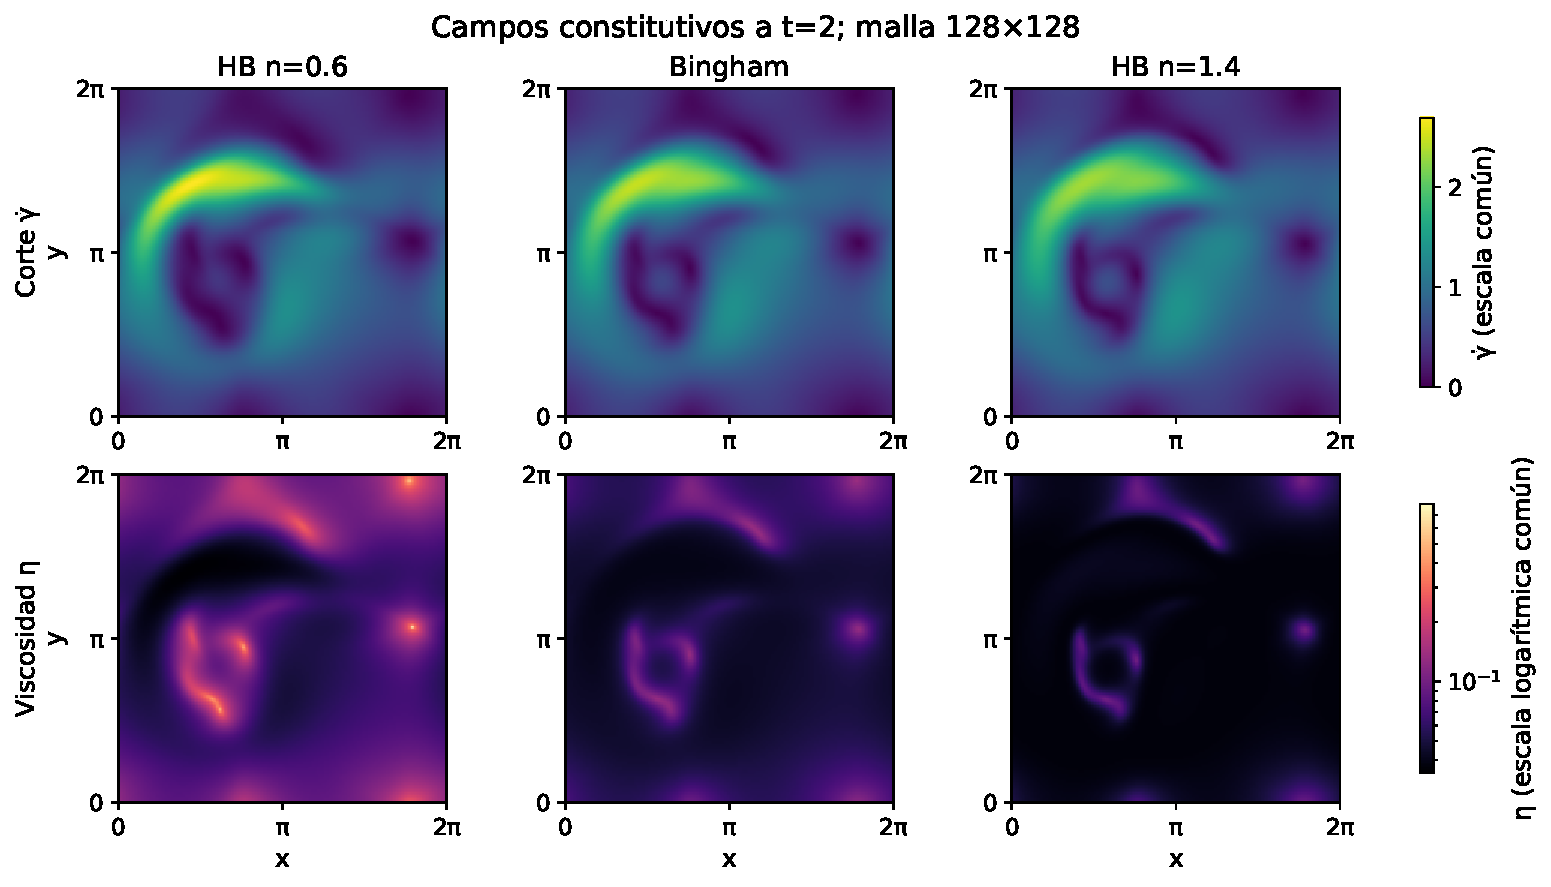
\includegraphics[width=\linewidth,height=.80\textwidth,keepaspectratio]{results/research/highres_viscoplastic_2026-10-14/figures/shear_viscosity_publication.pdf}
\caption{Tasa de corte y viscosidad aparente finales de los tres materiales en 128$^2$. La viscosidad usa una escala logarítmica común declarada; las magnitudes y sus barras se muestran por separado. Son campos constitutivos calculados, sin un tope artificial de viscosidad.}
\label{fig:vp-viscosity}\end{figure}
\end{landscape}
\clearpage
\clearpage
\begin{landscape}
\begin{figure}[p]\centering
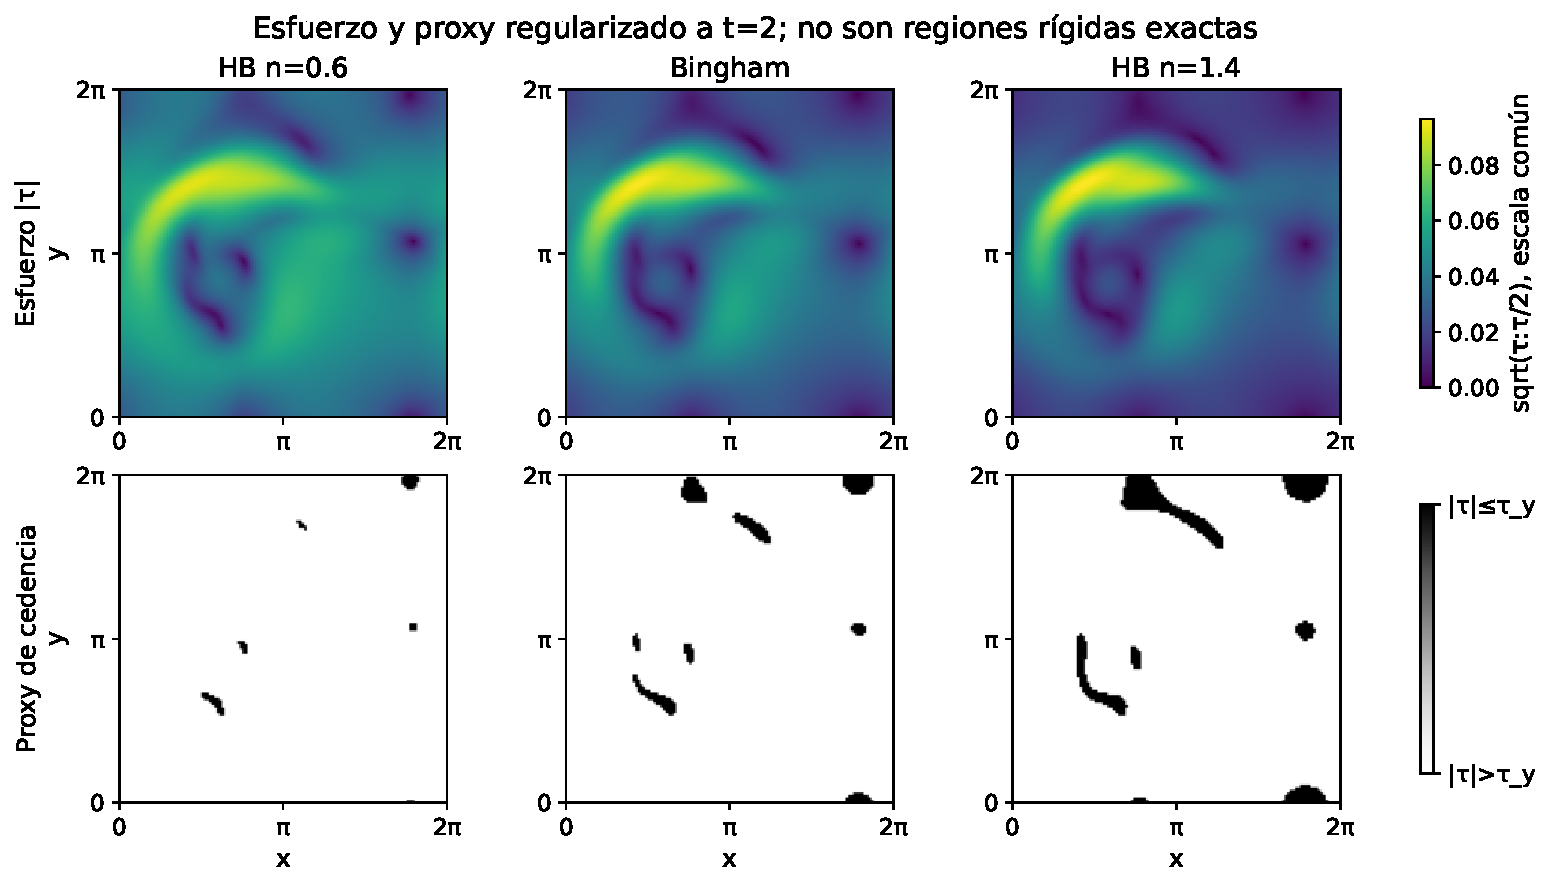
\includegraphics[width=\linewidth,height=.80\textwidth,keepaspectratio]{results/research/highres_viscoplastic_2026-10-14/figures/stress_yield_publication.pdf}
\caption{Esfuerzo y proxy de bajo esfuerzo respecto a $\tau_y$ al final en 128$^2$. El indicador regularizado no identifica regiones rígidas exactamente no cedidas. El modelo admite deformación incluso cuando el esfuerzo queda por debajo del umbral.}
\label{fig:vp-yield}\end{figure}
\end{landscape}
\clearpage
\clearpage
\begin{figure}[p]\centering
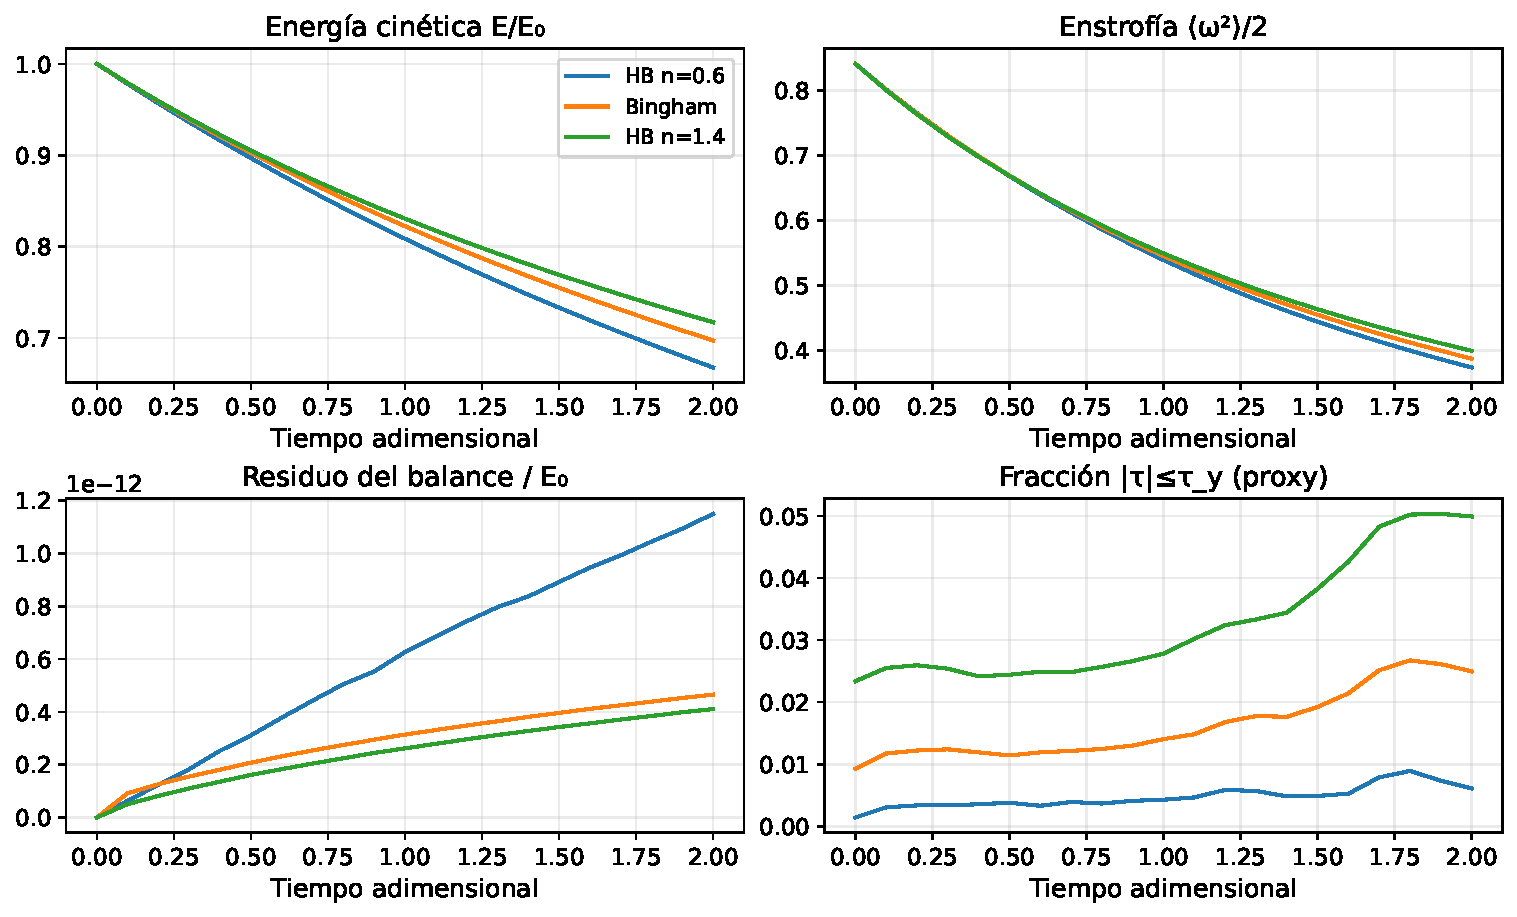
\includegraphics[width=\textwidth,height=.75\textheight,keepaspectratio]{results/research/highres_viscoplastic_2026-10-14/figures/diagnostics_publication.pdf}
\caption{Energía, enstrofía, disipación y defecto de balance de los tres materiales durante la evolución 128$^2$. El balance emplea cuadratura constitutiva con padding; la cuadratura en la malla de salida puede diferir. Los residuos se conservan en vez de reemplazarlos por conservación exacta.}
\label{fig:vp-diagnostics}\end{figure}
\clearpage
\clearpage
\begin{figure}[p]\centering
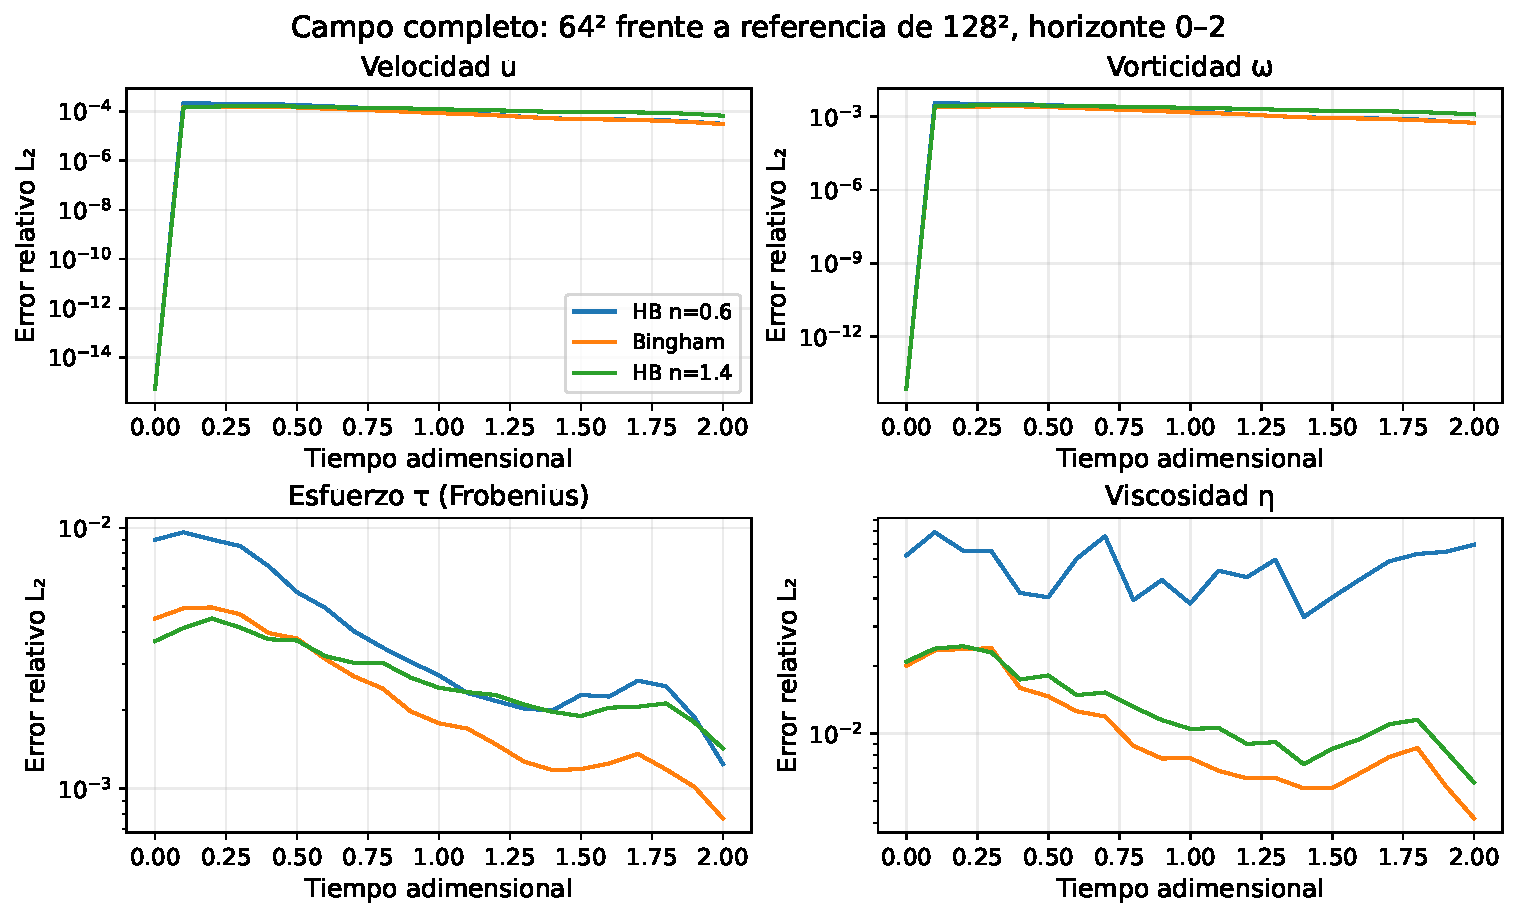
\includegraphics[width=\textwidth,height=.75\textheight,keepaspectratio]{results/research/highres_viscoplastic_2026-10-14/figures/full_field_refinement.pdf}
\caption{Errores completos durante 0$\leq$t$\leq$2: 64$^2$ frente a 128$^2$ en velocidad, vorticidad, esfuerzo tensorial de Frobenius y viscosidad aparente. El máximo temporal puede diferir del error final y revela gradientes constitutivos que la rapidez no permite evaluar.}
\label{fig:vp-full-refinement}\end{figure}
\clearpage
\clearpage
\begin{figure}[p]\centering
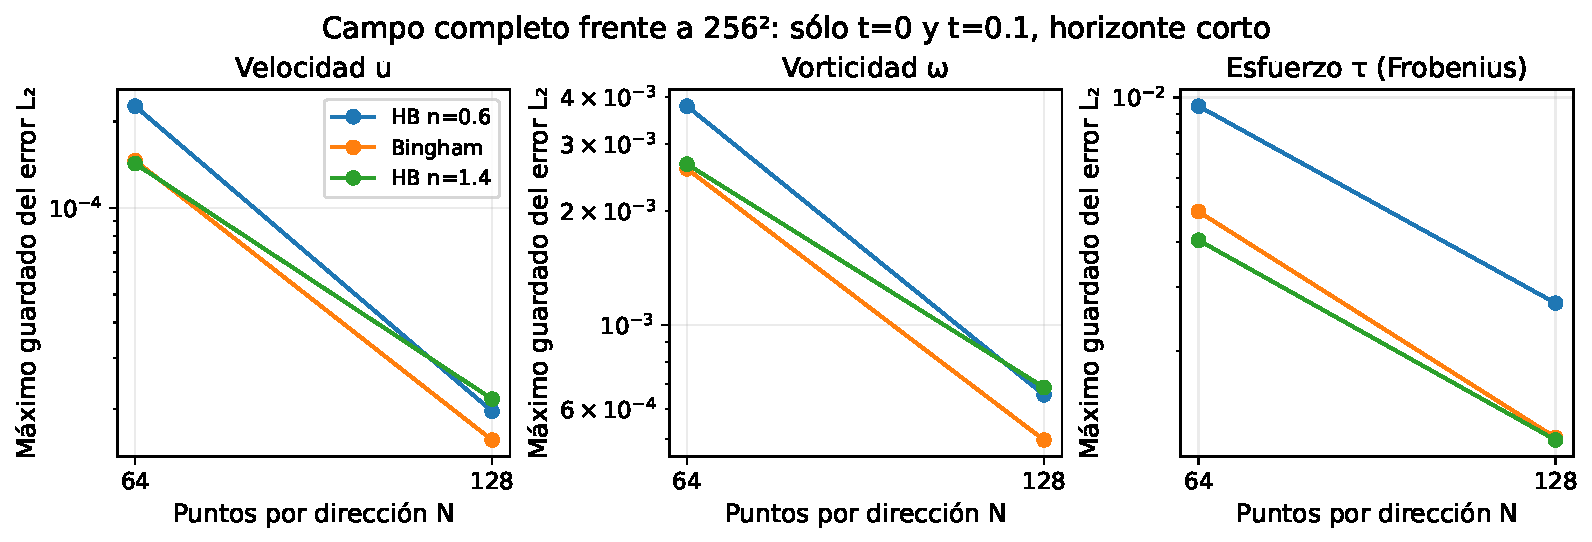
\includegraphics[width=\textwidth,height=.75\textheight,keepaspectratio]{results/research/highres_viscoplastic_2026-10-14/figures/spatial_refinement_publication.pdf}
\caption{Refinamiento espacial de horizonte corto: máximos sobre t=0 y t=0.1 de las soluciones 64$^2$ y 128$^2$ frente al campo completo 256$^2$. Estos dos instantes no establecen convergencia a lo largo de la evolución posterior hasta t=2.}
\label{fig:vp-short-refinement}\end{figure}
\clearpage
\begingroup\small\setlength{\tabcolsep}{3pt}
\begin{longtable}{@{}>{\raggedright\arraybackslash}p{3.8cm}>{\raggedright\arraybackslash}p{3.8cm}>{\raggedright\arraybackslash}p{3.7cm}>{\raggedright\arraybackslash}p{3.7cm}@{}}
\caption{HB adelgazante, control temporal a 128$^2$ hasta t=0.1; nominales 0.0004/0.0002 frente a 0.0001.}\\
\toprule
dt máximo real & dt máximo real ref. & Máx. error u & Máx. error $\omega$ \\
\midrule\endfirsthead
\toprule
dt máximo real & dt máximo real ref. & Máx. error u & Máx. error $\omega$ \\
\midrule\endhead
4.000e-04 & 1.000e-04 & 3.222e-11 \% & 8.043e-10 \% \\
2.000e-04 & 1.000e-04 & 5.504e-12 \% & 6.535e-11 \% \\
\bottomrule\end{longtable}\endgroup

La sensibilidad a padding, m y $\epsilon$ se registra en un archivo aparte. Aumentar el padding comprueba la cuadratura de la ley no polinómica; cambiar m o $\epsilon$ modifica la ley constitutiva regularizada. Son preguntas diferentes del refinamiento de malla. El padding 3/2 no elimina exactamente todo el aliasing de esta ley y la ausencia de un tope de viscosidad puede imponer pasos internos pequeños.

\clearpage
\subsection{\texorpdfstring{Reconstrucción en 128$^2$ y 256$^2$: conservar divergencia no basta}{Reconstrucción en 128 por 128 y 256 por 256: conservar divergencia no basta}}
Se ajustaron cinco variantes declaradas (observación, POD r=8, TLS-DMD r=8, TLS-DMD r=8 proyectado y TLS-DMD r=16 proyectado), dos contaminaciones y tres semillas de ruido en 128$^2$ y 256$^2$: 60 condiciones. El ruido tiene RMS relativo 20 \% y los rangos se fijaron sin seleccionar mediante la referencia limpia. La tarea es reconstrucción dentro del intervalo observado, no pronóstico. La proyección de Helmholtz y el corte 2/3 usan geometría periódica; no consultan el campo limpio.

El gaussiano IID se genera por celda: al refinar cambia la realización espacial y su contenido de altas frecuencias. Mantener su RMS de velocidad no mantiene el RMS de sus derivadas, por lo que la vorticidad ruidosa puede crecer con la resolución. El ruido espacial usa una realización maestra $256^2$, suavizada con un núcleo gaussiano de desviación $\sigma_{\mathrm{filtro}}=0.10$ y transferida a $128^2$ sin renormalizarla por malla. Ese ancho es del filtro, no de la autocorrelación: su desviación continua correspondiente sería $\sqrt{2}\sigma_{\mathrm{filtro}}\simeq0.1414$. Así se conserva una longitud física al comparar mallas.

\begingroup\small\setlength{\tabcolsep}{3pt}
\begin{longtable}{@{}>{\raggedright\arraybackslash}p{1.4cm}>{\raggedright\arraybackslash}p{2.2cm}>{\raggedright\arraybackslash}p{5.2cm}>{\raggedright\arraybackslash}p{3.1cm}>{\raggedright\arraybackslash}p{3.1cm}@{}}
\caption{Errores L2 de toda la ventana, mediana de tres semillas; no son máximos temporales ni intervalos de confianza.}\\
\toprule
Malla & Ruido & Estimador & Mediana error u & Mediana error $\omega$ \\
\midrule\endfirsthead
\toprule
Malla & Ruido & Estimador & Mediana error u & Mediana error $\omega$ \\
\midrule\endhead
128$^2$ & IID & Observación ruidosa & 20 \% & 487.8 \% \\
128$^2$ & IID & POD, r=8 & 8.907 \% & 215.4 \% \\
128$^2$ & IID & TLS-DMD, r=8 & 9.214 \% & 221.1 \% \\
128$^2$ & IID & TLS-DMD, r=8, proyectado & 4.553 \% & 99.18 \% \\
128$^2$ & IID & TLS-DMD, r=16, proyectado & 4.731 \% & 103.6 \% \\
128$^2$ & Espacial & Observación ruidosa & 20 \% & 94.58 \% \\
128$^2$ & Espacial & POD, r=8 & 9.459 \% & 43 \% \\
128$^2$ & Espacial & TLS-DMD, r=8 & 8.438 \% & 39.11 \% \\
128$^2$ & Espacial & TLS-DMD, r=8, proyectado & 6.172 \% & 39.11 \% \\
128$^2$ & Espacial & TLS-DMD, r=16, proyectado & 6.552 \% & 41.41 \% \\
256$^2$ & IID & Observación ruidosa & 20 \% & 982 \% \\
256$^2$ & IID & POD, r=8 & 8.894 \% & 434.1 \% \\
256$^2$ & IID & TLS-DMD, r=8 & 9.171 \% & 444.2 \% \\
256$^2$ & IID & TLS-DMD, r=8, proyectado & 4.557 \% & 199.6 \% \\
256$^2$ & IID & TLS-DMD, r=16, proyectado & 5.152 \% & 225.5 \% \\
256$^2$ & Espacial & Observación ruidosa & 20 \% & 94.58 \% \\
256$^2$ & Espacial & POD, r=8 & 9.459 \% & 43 \% \\
256$^2$ & Espacial & TLS-DMD, r=8 & 8.438 \% & 39.11 \% \\
256$^2$ & Espacial & TLS-DMD, r=8, proyectado & 6.172 \% & 39.11 \% \\
256$^2$ & Espacial & TLS-DMD, r=16, proyectado & 6.552 \% & 41.41 \% \\
\bottomrule\end{longtable}\endgroup

Los 60 ajustes finalizaron sin fallo de ejecución y 0/60 cumplen simultáneamente las puertas físicas declaradas: error de velocidad $\leq$15 \%, vorticidad $\leq$25 \%, divergencia adicional normalizada $\leq$0.1 y energía cinética $\leq$15 \%. La proyección reduce la divergencia al redondeo, pero el error de vorticidad sigue siendo demasiado alto incluso cuando el error de velocidad cae al entorno de 4–7 \%. Este resultado negativo evita confundir incompresibilidad geométrica con recuperación correcta de los gradientes.

\clearpage
\begin{landscape}
\begin{figure}[p]\centering
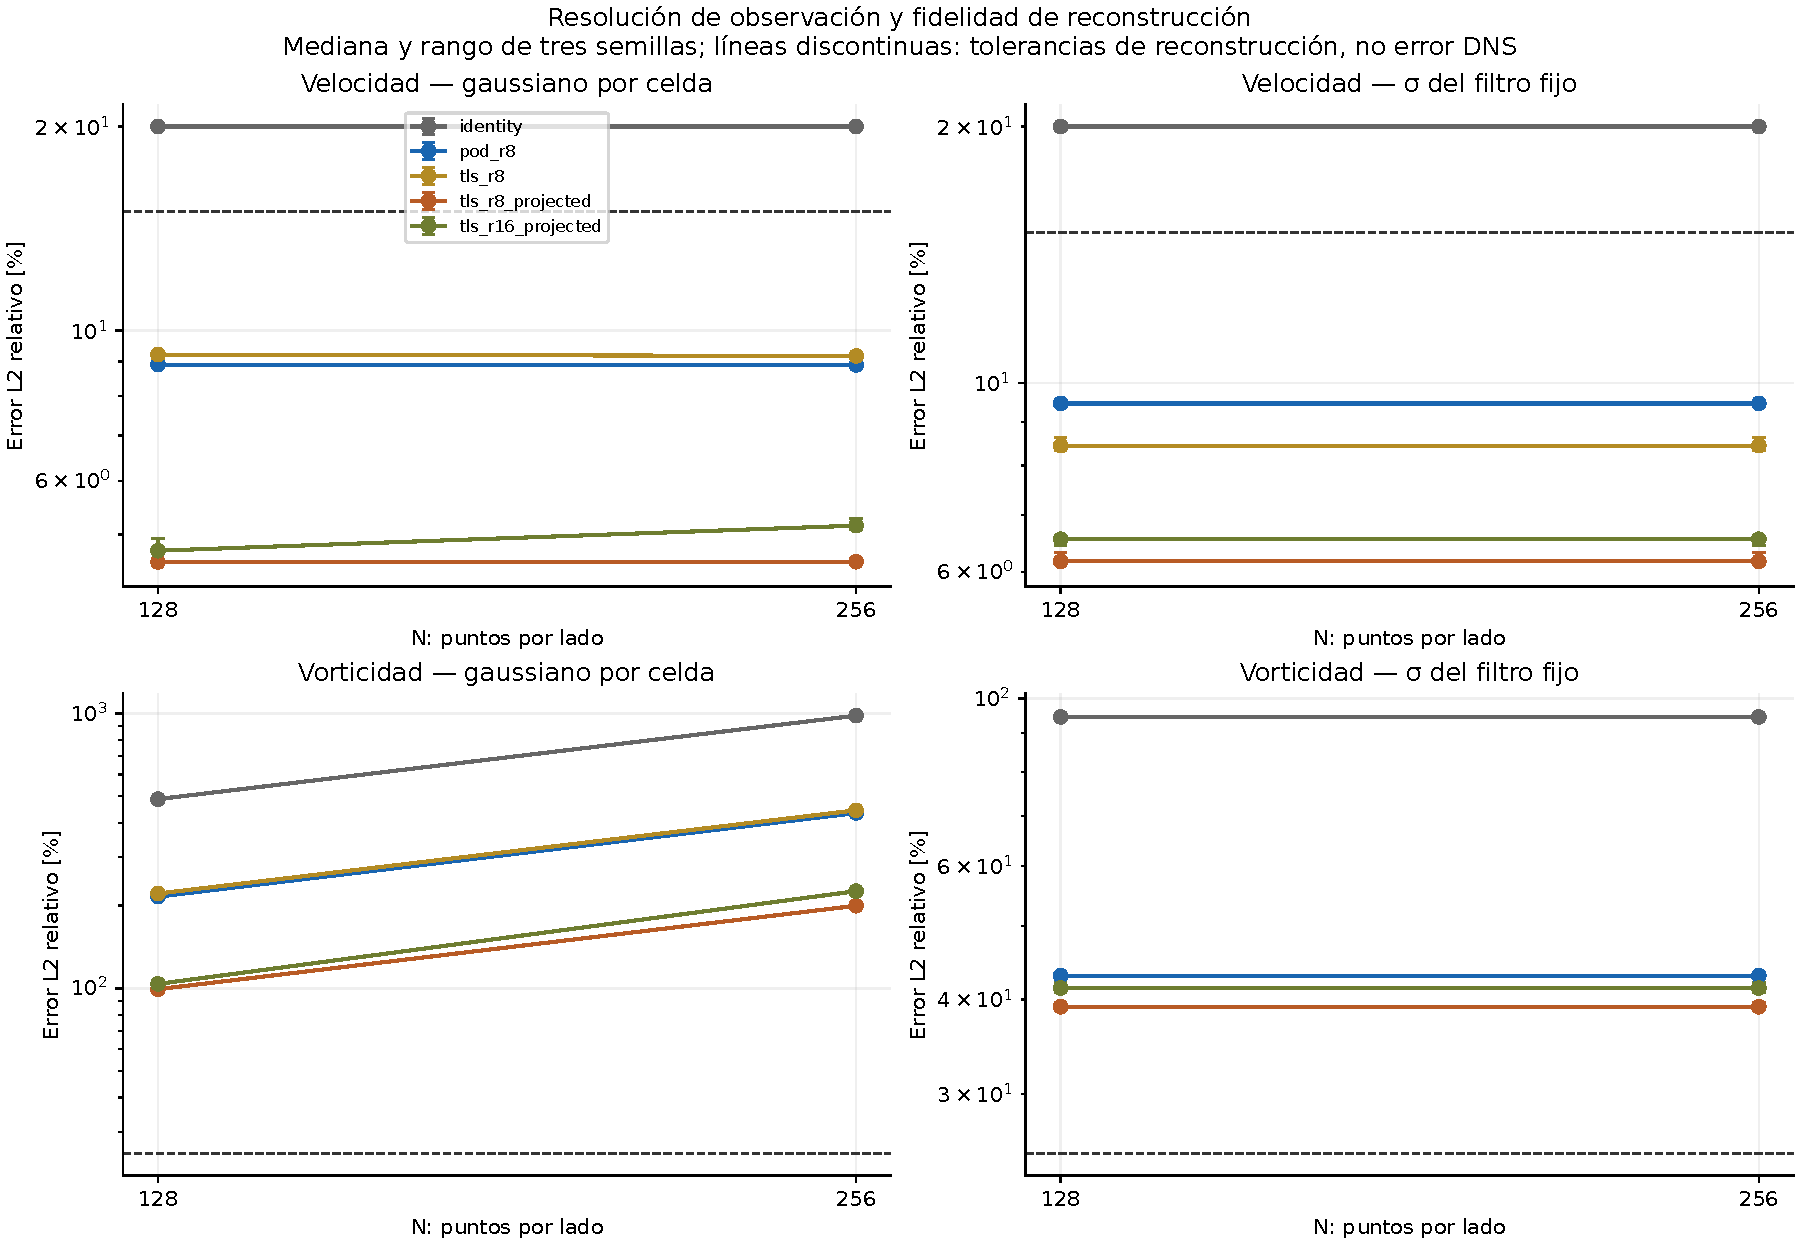
\includegraphics[width=\linewidth,height=.80\textwidth,keepaspectratio]{results/research/highres_reconstruction_2026-10-14/figures/noise_grid_comparison.pdf}
\caption{Reconstrucción en dos resoluciones y dos modelos de ruido: errores de velocidad y vorticidad para los cinco estimadores, con tres semillas. El ruido IID por celda introduce derivadas distintas al refinar; la contaminación espacial conserva su longitud mediante una realización maestra. Los puntos de tres semillas no constituyen un intervalo de confianza.}
\label{fig:reconstruction-noise}\end{figure}
\end{landscape}
\clearpage
\clearpage
\begin{landscape}
\begin{figure}[p]\centering
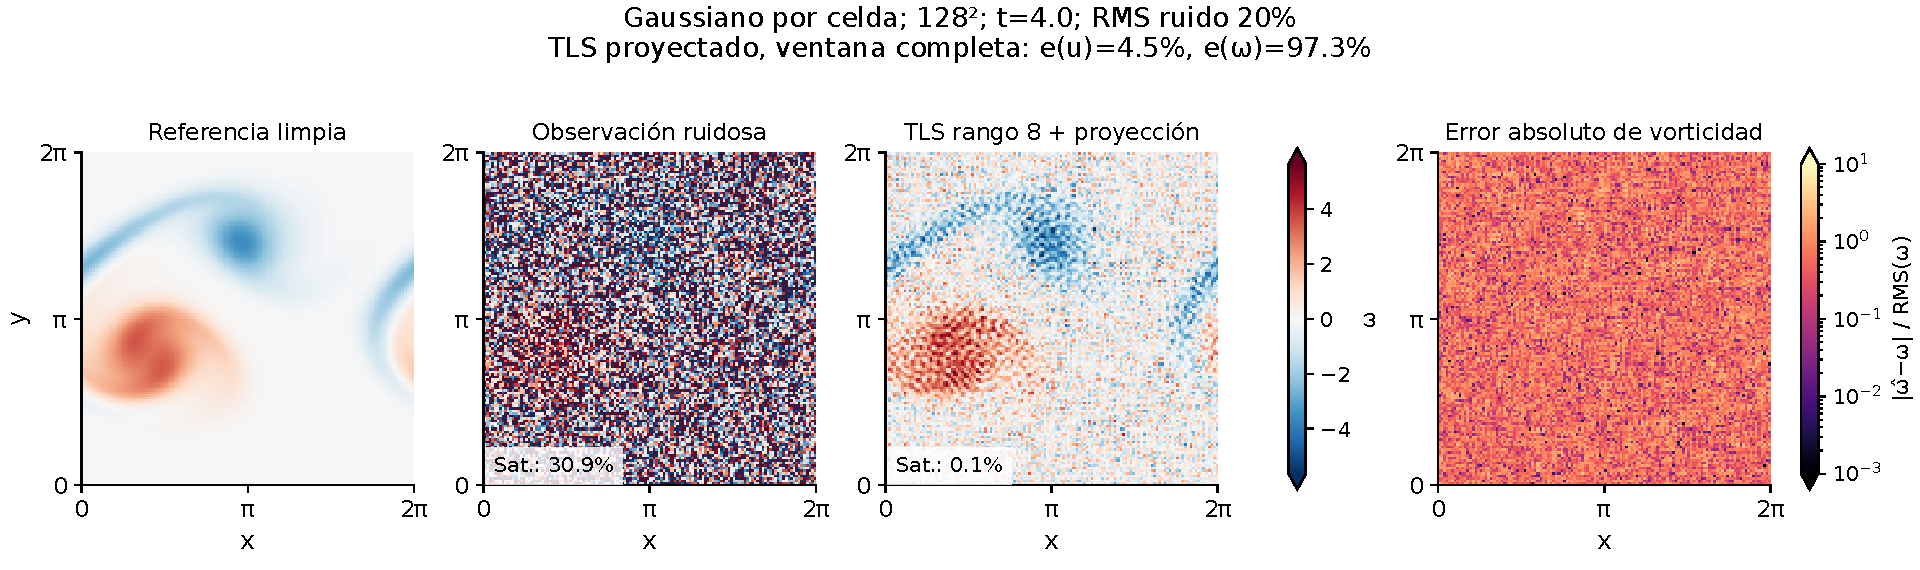
\includegraphics[width=\linewidth,height=.80\textwidth,keepaspectratio]{results/research/highres_reconstruction_2026-10-14/figures/gaussian_iid_128_frame_40.pdf}
\caption{Gaussiano por celda, 128$^2$, semilla 7, t=4: referencia limpia, observación, TLS-DMD de rango 8 proyectado y error de vorticidad. Los tres campos usan el mismo límite físico de color y declaran el porcentaje saturado; el error tiene escala logarítmica propia normalizada por RMS de vorticidad limpia. El error visualizado no demuestra aceptación física: la puerta de vorticidad falla.}
\label{fig:reconstruction-gaussian_iid}\end{figure}
\end{landscape}
\clearpage
\clearpage
\begin{landscape}
\begin{figure}[p]\centering
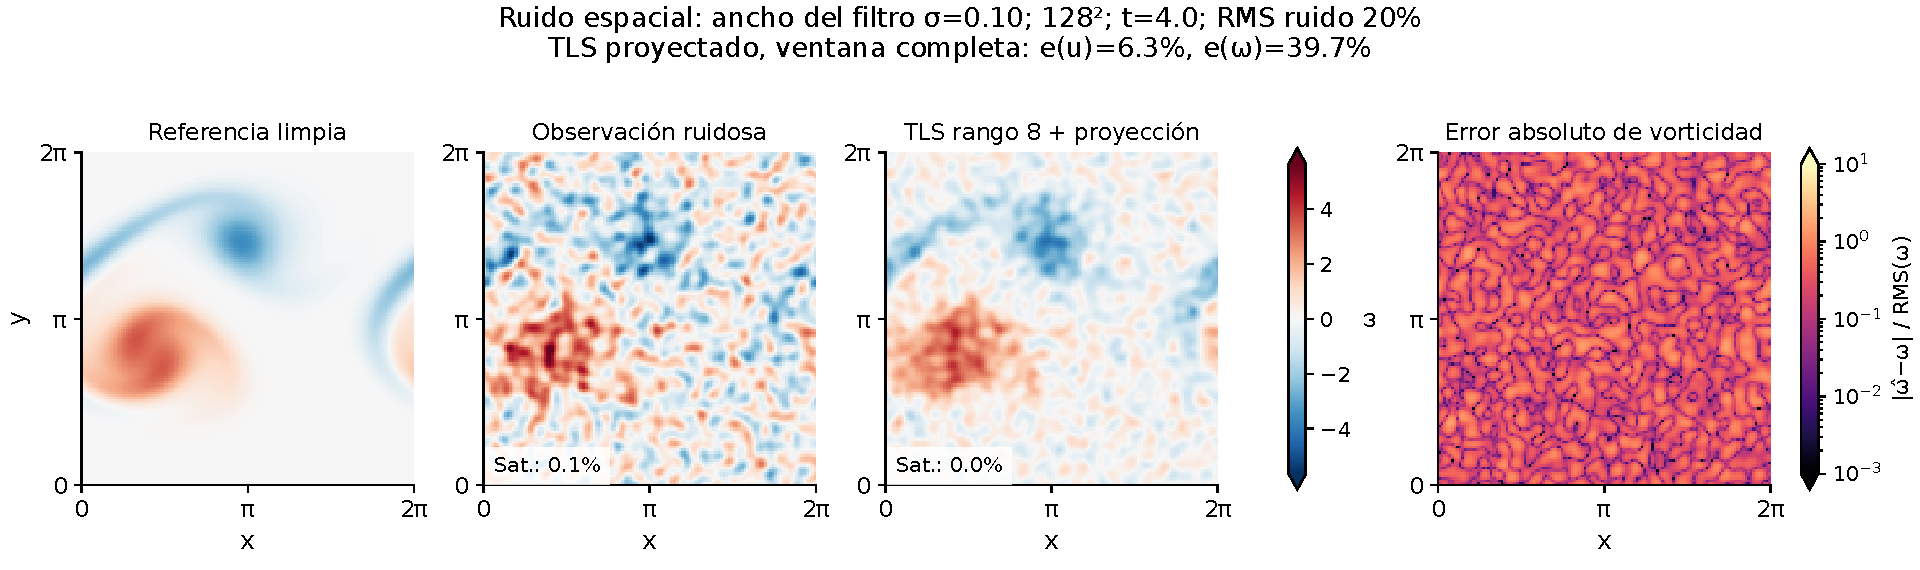
\includegraphics[width=\linewidth,height=.80\textwidth,keepaspectratio]{results/research/highres_reconstruction_2026-10-14/figures/spatial_fixed_length_128_frame_40.pdf}
\caption{Espacial, filtro de ancho fijo, 128$^2$, semilla 7, t=4: referencia limpia, observación, TLS-DMD de rango 8 proyectado y error de vorticidad. Los tres campos usan el mismo límite físico de color y declaran el porcentaje saturado; el error tiene escala logarítmica propia normalizada por RMS de vorticidad limpia. El error visualizado no demuestra aceptación física: la puerta de vorticidad falla.}
\label{fig:reconstruction-spatial_fixed_length}\end{figure}
\end{landscape}
\clearpage
\clearpage
\subsection{\texorpdfstring{Seguimiento exploratorio: conservar una longitud física de filtrado}{Seguimiento exploratorio: conservar una longitud física de filtrado}}
Después de observar las 60 condiciones que no alcanzaron la puerta física, se añadió un seguimiento exploratorio de ancho de banda. Usa las mismas realizaciones, semillas, campos y umbrales: no constituye prueba independiente ni selección ciega. El corte circular físico $k_c=10$ se fijó una vez a partir de $1/\sigma_{\mathrm{filtro}}$ con ancho sintético conocido 0.10, sin barrer cortes para minimizar el error limpio. En el caso IID se aplica la misma escala asumida, pues el ruido por celda no posee ese ancho físico.

Ambas opciones proyectan la velocidad a divergencia cero y eliminan números de onda superiores al mismo corte físico en 128$^2$ y 256$^2$. Una aplica el prior directamente a la observación; la otra lo combina con TLS-DMD de rango 8. Mantener ese control permite atribuir qué parte de la mejora procede del prior espacial y cuál del ajuste temporal. Filtrar puede reducir ruido y también borrar estructuras físicas reales: este compromiso se mide frente a los campos limpios completos, sin filtrar la referencia.

\begingroup\small\setlength{\tabcolsep}{3pt}
\begin{longtable}{@{}>{\raggedright\arraybackslash}p{1.0887cm}>{\raggedright\arraybackslash}p{1.7815cm}>{\raggedright\arraybackslash}p{5.1465cm}>{\raggedright\arraybackslash}p{2.6722cm}>{\raggedright\arraybackslash}p{2.6722cm}>{\raggedright\arraybackslash}p{1.4846cm}@{}}
\caption{Seguimiento posterior al resultado inicial: errores de toda la ventana y tres semillas, referencia limpia completa.}\\
\toprule
Malla & Ruido & Estimador, corte físico 10 & Mediana error u & Mediana error $\omega$ & Puerta física \\
\midrule\endfirsthead
\toprule
Malla & Ruido & Estimador, corte físico 10 & Mediana error u & Mediana error $\omega$ & Puerta física \\
\midrule\endhead
128$^2$ & IID & Observación + proyección + corte & 2.02 \% & 10.03 \% & 3/3 \\
128$^2$ & IID & TLS-DMD r=8 + proyección + corte & 1.933 \% & 8.171 \% & 3/3 \\
128$^2$ & Espacial & Observación + proyección + corte & 11.29 \% & 49.23 \% & 0/3 \\
128$^2$ & Espacial & TLS-DMD r=8 + proyección + corte & 5.166 \% & 22.17 \% & 3/3 \\
256$^2$ & IID & Observación + proyección + corte & 1.088 \% & 5.867 \% & 3/3 \\
256$^2$ & IID & TLS-DMD r=8 + proyección + corte & 1.729 \% & 7.161 \% & 3/3 \\
256$^2$ & Espacial & Observación + proyección + corte & 11.29 \% & 49.23 \% & 0/3 \\
256$^2$ & Espacial & TLS-DMD r=8 + proyección + corte & 5.166 \% & 22.17 \% & 3/3 \\
\bottomrule\end{longtable}\endgroup

El seguimiento completó 24 condiciones y 18/24 alcanzan las puertas declaradas. Ese recuento se mantiene separado del resultado original 0/60. El corte y su justificación se definieron después de observar el fallo, por lo que el resultado requiere validación posterior con condiciones nuevas y una escala de filtrado estimable sin conocer el modelo de ruido sintético. Tampoco demuestra éxito de pronóstico, de RPCA ni robustez universal ante ruido temporal o deriva de sensores.

Con ruido IID en 256$^2$, el control espacial por sí solo da mediana de error de vorticidad 5.867 \%, frente a 7.161 \% al combinarlo con TLS-DMD. En estas condiciones el control simple es mejor en ese observable. Con ruido espacial en 128$^2$, las medianas correspondientes son 49.23 \% y 22.17 \%. Aquí el ajuste temporal aporta una mejora. Son contrastes descriptivos del mismo banco reutilizado, no evidencia de un ganador general ni una regla de selección ya validada.

\clearpage
\begin{landscape}
\begin{figure}[p]\centering
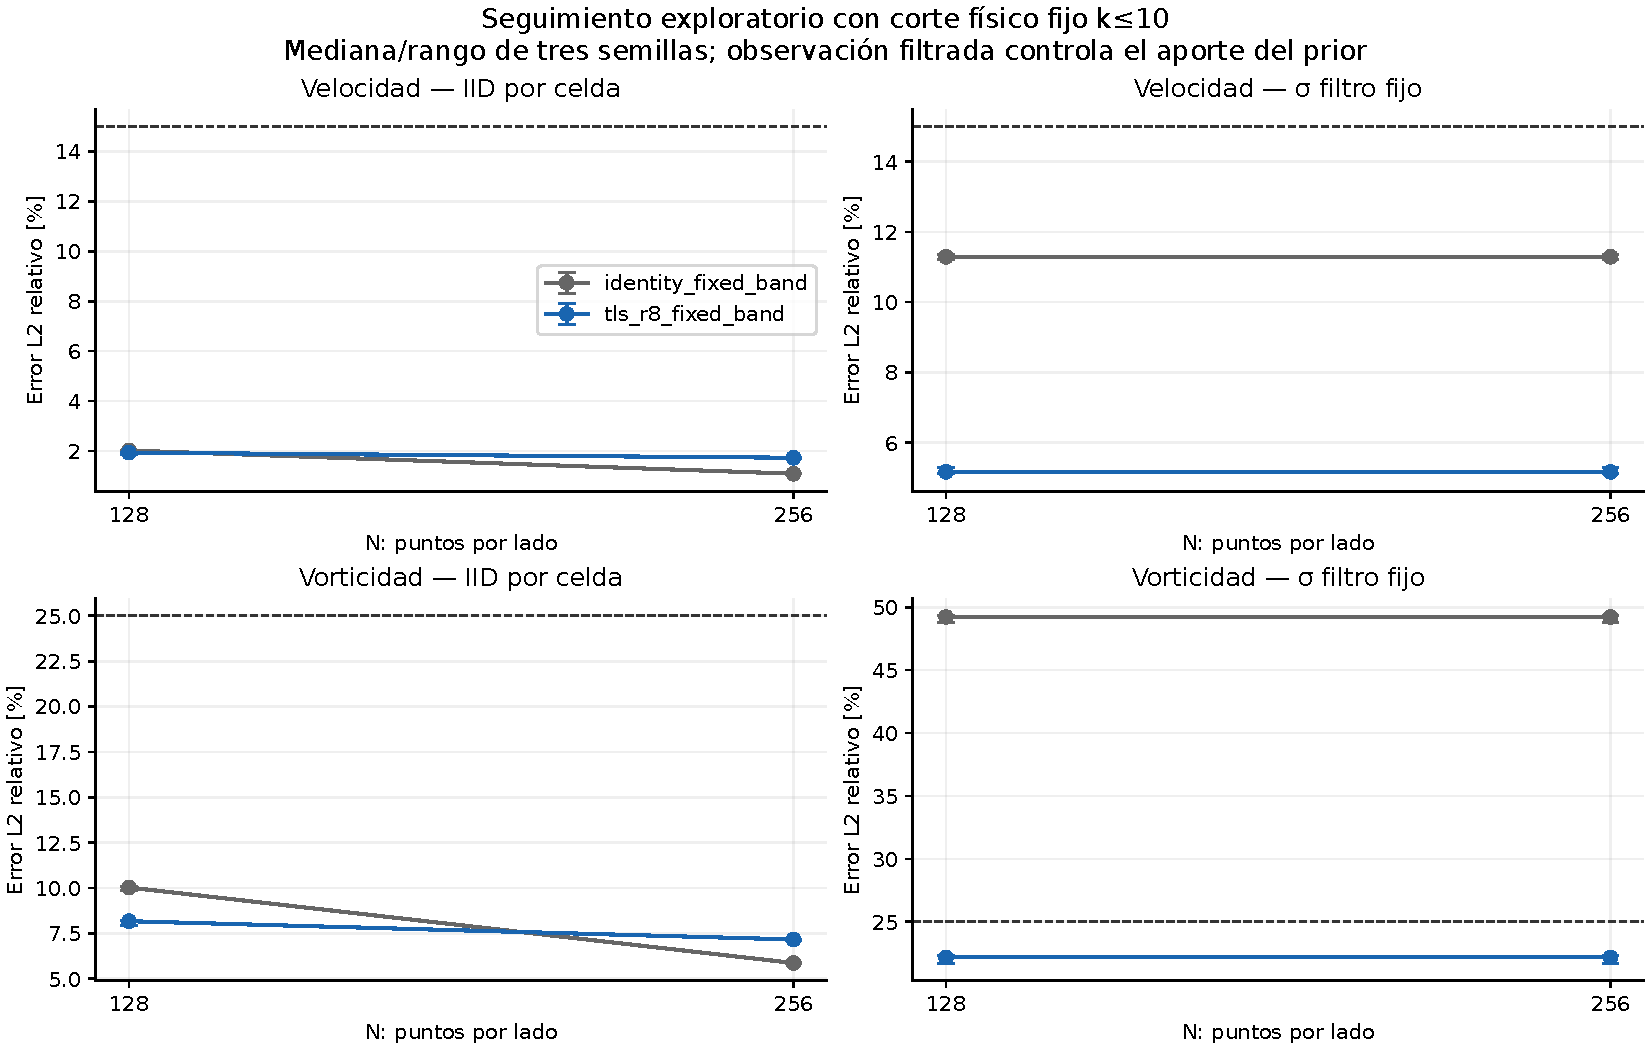
\includegraphics[width=\linewidth,height=.80\textwidth,keepaspectratio]{results/research/highres_fixed_bandwidth_2026-10-14/figures/noise_grid_comparison.pdf}
\caption{Seguimiento exploratorio de ancho fijo: comparación entre el prior aplicado a la observación y el mismo prior combinado con TLS-DMD r=8, en dos mallas y dos ruidos. El corte físico permanece en $k_c$=10; la referencia limpia conserva todas sus escalas y los puntos proceden de las tres semillas reutilizadas.}
\label{fig:fixed-bandwidth-comparison}\end{figure}
\end{landscape}
\clearpage
\clearpage
\begin{landscape}
\begin{figure}[p]\centering
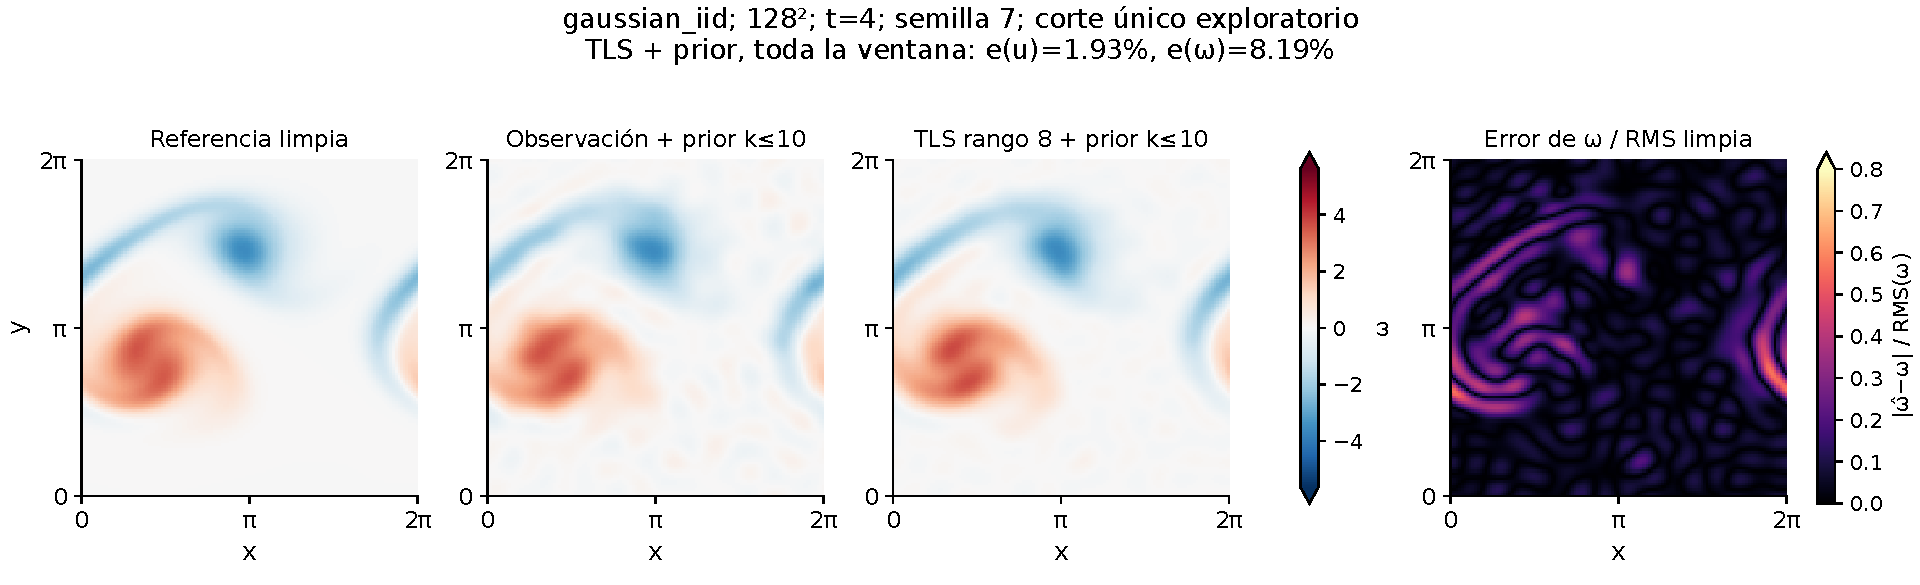
\includegraphics[width=\linewidth,height=.80\textwidth,keepaspectratio]{results/research/highres_fixed_bandwidth_2026-10-14/figures/gaussian_iid_128_bandwidth_comparison.pdf}
\caption{Gaussiano por celda, 128$^2$: campos calculados en el seguimiento de ancho de banda fijo. El control de observación filtrada y el ajuste TLS-DMD comparten proyección y corte físico 10. Las barras distinguen campo y error, y permiten inspeccionar el ruido eliminado junto con las estructuras físicas que también puede suprimir el prior.}
\label{fig:fixed-bandwidth-gaussian_iid}\end{figure}
\end{landscape}
\clearpage
\clearpage
\begin{landscape}
\begin{figure}[p]\centering
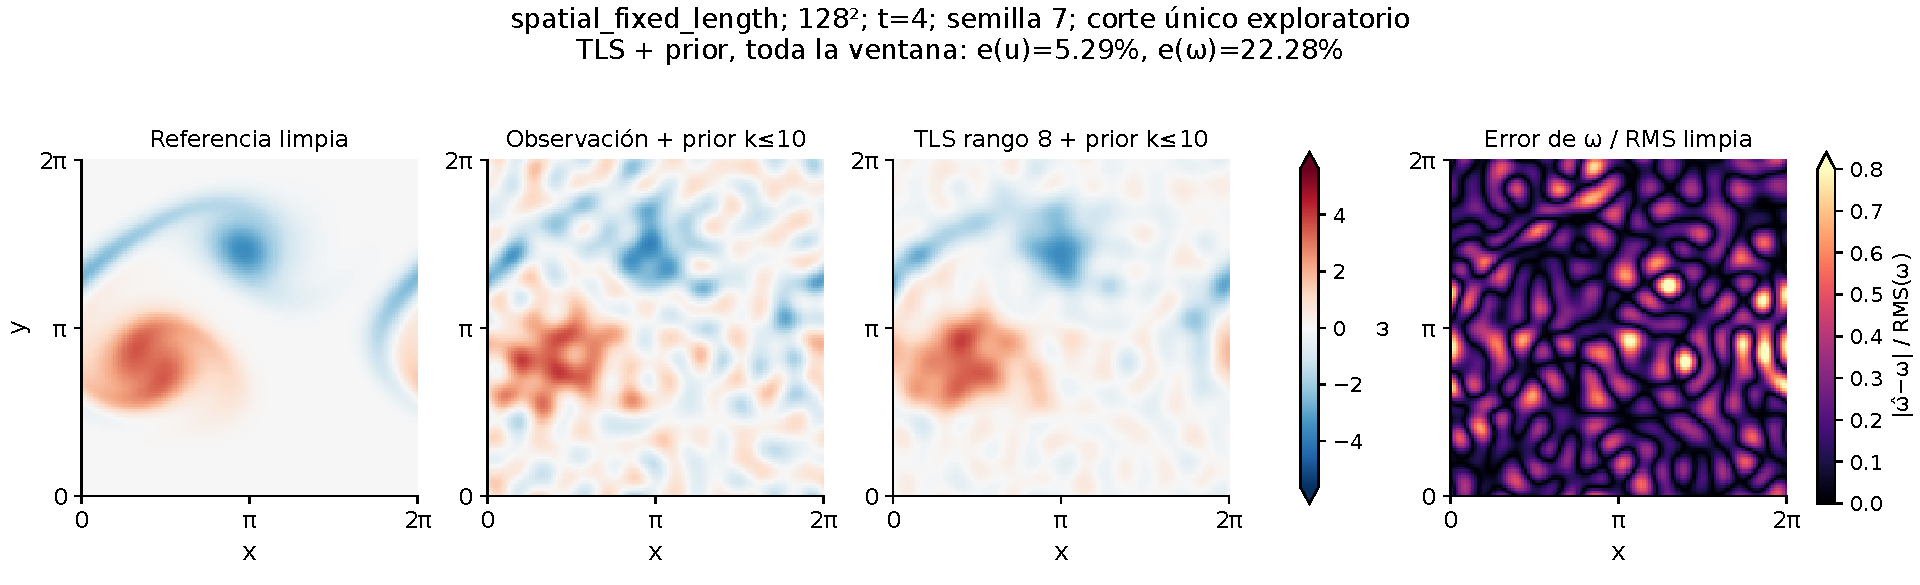
\includegraphics[width=\linewidth,height=.80\textwidth,keepaspectratio]{results/research/highres_fixed_bandwidth_2026-10-14/figures/spatial_fixed_length_128_bandwidth_comparison.pdf}
\caption{Espacial, filtro de ancho fijo, 128$^2$: campos calculados en el seguimiento de ancho de banda fijo. El control de observación filtrada y el ajuste TLS-DMD comparten proyección y corte físico 10. Las barras distinguen campo y error, y permiten inspeccionar el ruido eliminado junto con las estructuras físicas que también puede suprimir el prior.}
\label{fig:fixed-bandwidth-spatial_fixed_length}\end{figure}
\end{landscape}
\clearpage
\clearpage
\subsection{\texorpdfstring{Lectura conjunta y límites que conserva esta evidencia}{Lectura conjunta y límites que conserva esta evidencia}}
La malla 512$^2$ newtoniana hace comprobable la convergencia del banco suave estudiado y permite ver su evolución con detalle. Los campos poliméricos y de viscosidad pueden requerir más resolución que la velocidad; por ello se mantienen las comparaciones de C$-$I, esfuerzo y viscosidad, sus máximos temporales y los defectos de balance. Las figuras aportan estructura y contexto; las conclusiones de resolución provienen de comparaciones entre integraciones independientes.

La evidencia se limita a flujos bidimensionales, periódicos, sin forzamiento y de densidad constante en los parámetros e intervalos ejecutados. El balance de materia con $\rho$=1 no comprueba evolución de densidad compresible. Permanecen pendientes las estelas externas con cilindro y paredes, el horizonte largo viscoplástico frente a 256$^2$ o superior, el régimen de alto Weissenberg, la validación experimental y las estructuras tridimensionales. Tampoco se ha certificado caos. La dificultad previa con ruido temporal y deriva de sensores permanece documentada; aumentar la malla no corrige por sí solo su identificabilidad.

Las tablas se generan exclusivamente cuando las cinco campañas tienen un cierre completo y las figuras requeridas existen. Los manifiestos conservan parámetros, SHA-256 de fuentes, datos o archivos y pasos internos. La revisión independiente comprueba transferencia, normalización espectral, referencias analíticas y archivos guardados. Esta trazabilidad permite reproducir el resultado y distinguir cada tipo de error.

\clearpage
\paragraph{Archivos reproducibles.}
Las animaciones GIF y las fuentes de estas 28 ilustraciones se enlazan en \path{docs/research/HIGHRES_RESULTS.md}. La sección se regenera mediante \path{python/scripts/build_highres_chapter.py} y requiere el cierre completo de las cinco campañas.


\section{Límites comunes de interpretación}
Una ventaja de un método bajo una distribución no acredita superioridad
en todas las demás. El promedio sobre casos analíticos estacionarios,
campos no lineales y un LBM no validado puede reflejar su mezcla; por eso
las comparaciones físicas se leen primero por caso y contaminación.
Tres semillas aportan una exploración inicial, sin representar toda la
variabilidad posible de la medición.

El error de vorticidad depende de la derivación y resolución; los
residuos adicionales aíslan alteraciones de reconstrucción respecto al
campo limpio, pero heredan sus limitaciones. Copiar la densidad permite
diagnosticar velocidad con una hipótesis de densidad conocida, no
recuperar densidad corrupta. El balance neto de flujo no sustituye las
comprobaciones locales de continuidad y pared.

La campaña de reconstrucción ajusta el intervalo observado y la campaña
cronológica evalúa un futuro separado. No se ejecutaron entrenamiento
profundo, online, GPU ni estelas externas de cilindro Oldroyd-B/FENE-P/EVP.
Los nuevos campos periódicos tienen memoria constitutiva o esfuerzo variable,
pero no reproducen por sí solos una calle de vórtices ni demuestran caos.
Los residuos constitutivos y de cuadratura no se sustituyen por cero.

\chapter{Conclusiones y líneas de trabajo futuro}
\section{Conclusiones metodológicas y alcance}
La campaña de mayor resolución muestra que la suficiencia depende de la
magnitud que se quiere observar. Frente a $512^2$, el caso multiescala en
$64^2$ tiene un error máximo de velocidad de $0.2007\%$, pero $1.312\%$ en
vorticidad; en $128^2$ esta última diferencia baja a $0.03032\%$. Las
imágenes y los espectros acompañan esa comparación, sin sustituirla.

En Oldroyd-B, frente a $256^2$, la velocidad de $128^2$ difiere apenas
$0.0008872\%$ mientras que conformación y esfuerzo difieren $4.383\%$.
FENE-P alcanza $0.1165\%$ en esfuerzo bajo los mismos parámetros nominales.
La cola tensorial de Oldroyd-B en $256^2$ todavía exige una referencia
superior antes de afirmar resolución constitutiva completa. En HB adelgazante,
la viscosidad aparente conserva $5.023\%$ de diferencia $128^2\to256^2$ en
la prueba corta; esa referencia no valida todo el horizonte largo.

Las 60 reconstrucciones de mayor malla incumplen los umbrales físicos pese
a reducir error de velocidad. El seguimiento exploratorio de banda física
fija alcanza 18 aceptaciones de 24, conservando un control de filtrado directo.
En gaussiano IID sobre $256^2$, ese control supera a TLS-DMD en vorticidad:
la mejora corresponde al conjunto de supuestos y operaciones, y no prueba
una ventaja universal del modelo dinámico. Una validación independiente
de ese nuevo prior permanece pendiente.

La ampliación establece una comparación verificable entre estructura de
contaminación, estimador, referencia física y recursos. El juicio de éxito
separa convergencia del algoritmo, fidelidad de reconstrucción,
conservación observada y costo. Un único tiempo o error escalar no
resuelve todas estas preguntas.

Las conclusiones numéricas se limitan a los artefactos del
capítulo~\ref{chap:results}. No se infiere la superioridad universal de
RPCA ni la inutilidad general de DMD a partir del estudio impulsivo
o del piloto. La SVD, los modelos dispersos y los ajustes
dinámicos tienen hipótesis y objetivos diferentes; sus fallos y
tradeoffs deben permanecer documentados.

El marco académico combina LBM--RPCA--DMD con pruebas de reconstrucción y física. No se reclama primera aplicación de DMD a
fluidos viscoelásticos o EVP. Las referencias de canal y los nuevos flujos periódicos bidimensionales
amplían las constitutivas observadas. Los estudios de refinamiento respaldan
regímenes concretos; no certifican una estela externa de cilindro, alto
Weissenberg ni una transición turbulenta tridimensional.

\section{Pronóstico y generalización fuera del ajuste}
La campaña cronológica ejecutada utiliza entrenamiento, validación y prueba
sin snapshots futuros durante la limpieza. Su selección ruidosa mejora la
persistencia en parte del banco, pero conserva errores altos de vorticidad en
flujos no lineales. El siguiente paso es evaluar horizontes más largos,
transferencia a condiciones no usadas en ajuste y cobertura de incertidumbre
cuando el método la entregue. El costo debe incluir entrenamiento y reajustes;
su amortización requiere declarar cuántas predicciones se producen.

Se amplían niveles de intensidad, rangos y correlaciones mediante la
configuración de resolución/rango. El ruido heteroscedástico, las colas pesadas y la deriva de sensor ya se
incluyeron en la ampliación. La deriva y la correlación temporal no alcanzan
las tolerancias de reconstrucción en este banco, y requieren modelos de
sesgo/memoria más específicos. Los datos faltantes y las perturbaciones de
forzado siguen pendientes de diseños separados. Los datos faltantes se representan con máscara y no se
convierten automáticamente en ceros observados. La selección de
hiperparámetros utiliza validación separada y presupuesto comparable.

\section{Wakes no newtonianos y campaña HPC pendiente}
La extensión física avanza por etapas: benchmark newtoniano con
geometría/fronteras reproducidas, HB/Bingham regularizado en wake,
Oldroyd-B/FENE-P con tensor de conformación y, finalmente,
Saramito--Herschel--Bulkley EVP. Los parámetros Re, Wi, Bn, $\beta$,
extensibilidad y regularización se declaran junto con sus escalas.

El manifiesto externo toma $Re=100$ como línea de comparación con
antecedentes, sin sustituir la verificación del solver. Antes de analizar
modos se exige refinamiento espacial/temporal, sensibilidad a dominio y
fronteras, resolución de capas de esfuerzo y checks constitutivos.
Log-conformation aporta estabilización, pero no elimina esas
necesidades. La campaña de \citet{corrochano2026evp} ilustra la escala
de cómputo de wakes EVP; citarla o preparar un manifiesto no significa
haber reproducido sus simulaciones.

La integración de RheoTool o Basilisk fija versión/commit,
configuración, dependencias, licencia y pruebas del solver. Los
manifiestos mantienen estado pendiente hasta producir y verificar
campos. Una viscosidad espacial variable no reemplaza la ecuación de
memoria de esfuerzos ni la constitutiva EVP. Clasificar un campo como
caótico requiere evidencia dinámica; la apariencia de una imagen no
es una prueba.

\section{Escala 3D, GPU, online y validación PIV}
Los campos 3D, los modelos incrementales y la aceleración GPU se
abordan después de verificar precisión y conservación. La SVD
truncada/aleatoria, las pasadas sobre datos y el movimiento de memoria
se comparan explícitamente. Un objetivo de reconstrucción sub-segundo requiere medición propia; no se deriva automáticamente de utilizar una GPU.

La validación con PIV real requiere calibración de incertidumbre,
máscaras de observación y datos que permitan evaluar sin una
referencia limpia perfecta. Las comparaciones con autoencoders u otros
modelos aprendidos separan realizaciones, regímenes y conjuntos de
entrenamiento/test, contabilizan costo de entrenamiento y reportan
degradación física además de error visual. La integración de uso se
apoya en esquemas de datos y scripts reproducibles, una vez validadas
las etapas científicas.

\backmatter
\bibliographystyle{plainnat}
\bibliography{docs/research/references}
\end{document}
